\documentclass[twoside]{book}

% Packages required by doxygen
\usepackage{fixltx2e}
\usepackage{calc}
\usepackage{doxygen}
\usepackage[export]{adjustbox} % also loads graphicx
\usepackage{graphicx}
\usepackage[utf8]{inputenc}
\usepackage{makeidx}
\usepackage{multicol}
\usepackage{multirow}
\PassOptionsToPackage{warn}{textcomp}
\usepackage{textcomp}
\usepackage[nointegrals]{wasysym}
\usepackage[table]{xcolor}

% Font selection
\usepackage[T1]{fontenc}
\usepackage[scaled=.90]{helvet}
\usepackage{courier}
\usepackage{amssymb}
\usepackage{sectsty}
\renewcommand{\familydefault}{\sfdefault}
\allsectionsfont{%
  \fontseries{bc}\selectfont%
  \color{darkgray}%
}
\renewcommand{\DoxyLabelFont}{%
  \fontseries{bc}\selectfont%
  \color{darkgray}%
}
\newcommand{\+}{\discretionary{\mbox{\scriptsize$\hookleftarrow$}}{}{}}

% Page & text layout
\usepackage{geometry}
\geometry{%
  a4paper,%
  top=2.5cm,%
  bottom=2.5cm,%
  left=2.5cm,%
  right=2.5cm%
}
\tolerance=750
\hfuzz=15pt
\hbadness=750
\setlength{\emergencystretch}{15pt}
\setlength{\parindent}{0cm}
\setlength{\parskip}{3ex plus 2ex minus 2ex}
\makeatletter
\renewcommand{\paragraph}{%
  \@startsection{paragraph}{4}{0ex}{-1.0ex}{1.0ex}{%
    \normalfont\normalsize\bfseries\SS@parafont%
  }%
}
\renewcommand{\subparagraph}{%
  \@startsection{subparagraph}{5}{0ex}{-1.0ex}{1.0ex}{%
    \normalfont\normalsize\bfseries\SS@subparafont%
  }%
}
\makeatother

% Headers & footers
\usepackage{fancyhdr}
\pagestyle{fancyplain}
\fancyhead[LE]{\fancyplain{}{\bfseries\thepage}}
\fancyhead[CE]{\fancyplain{}{}}
\fancyhead[RE]{\fancyplain{}{\bfseries\leftmark}}
\fancyhead[LO]{\fancyplain{}{\bfseries\rightmark}}
\fancyhead[CO]{\fancyplain{}{}}
\fancyhead[RO]{\fancyplain{}{\bfseries\thepage}}
\fancyfoot[LE]{\fancyplain{}{}}
\fancyfoot[CE]{\fancyplain{}{}}
\fancyfoot[RE]{\fancyplain{}{\bfseries\scriptsize Generated by Doxygen }}
\fancyfoot[LO]{\fancyplain{}{\bfseries\scriptsize Generated by Doxygen }}
\fancyfoot[CO]{\fancyplain{}{}}
\fancyfoot[RO]{\fancyplain{}{}}
\renewcommand{\footrulewidth}{0.4pt}
\renewcommand{\chaptermark}[1]{%
  \markboth{#1}{}%
}
\renewcommand{\sectionmark}[1]{%
  \markright{\thesection\ #1}%
}

% Indices & bibliography
\usepackage{natbib}
\usepackage[titles]{tocloft}
\setcounter{tocdepth}{3}
\setcounter{secnumdepth}{5}
\makeindex

% Hyperlinks (required, but should be loaded last)
\usepackage{ifpdf}
\ifpdf
  \usepackage[pdftex,pagebackref=true]{hyperref}
\else
  \usepackage[ps2pdf,pagebackref=true]{hyperref}
\fi
\hypersetup{%
  colorlinks=true,%
  linkcolor=blue,%
  citecolor=blue,%
  unicode%
}

% Custom commands
\newcommand{\clearemptydoublepage}{%
  \newpage{\pagestyle{empty}\cleardoublepage}%
}

\usepackage{caption}
\captionsetup{labelsep=space,justification=centering,font={bf},singlelinecheck=off,skip=4pt,position=top}

%===== C O N T E N T S =====

\begin{document}

% Titlepage & ToC
\hypersetup{pageanchor=false,
             bookmarksnumbered=true,
             pdfencoding=unicode
            }
\pagenumbering{alph}
\begin{titlepage}
\vspace*{7cm}
\begin{center}%
{\Large Chor Police \\[1ex]\large 11 }\\
\vspace*{1cm}
{\large Generated by Doxygen 1.8.13}\\
\end{center}
\end{titlepage}
\clearemptydoublepage
\pagenumbering{roman}
\tableofcontents
\clearemptydoublepage
\pagenumbering{arabic}
\hypersetup{pageanchor=true}

%--- Begin generated contents ---
\chapter{R\+E\+A\+D\+ME}
\label{md__r_e_a_d_m_e}
\Hypertarget{md__r_e_a_d_m_e}
\href{https://travis-ci.com/IITH-SBJoshi/concurrency-11}{\tt } \href{https://www.codacy.com?utm_source=github.com&amp;utm_medium=referral&amp;utm_content=vijayphoenix/Car-racing-game&amp;utm_campaign=Badge_Grade}{\tt }

\mbox{[} \mbox{]} Create a to-\/do List. 
\chapter{Hierarchical Index}
\section{Class Hierarchy}
This inheritance list is sorted roughly, but not completely, alphabetically\+:\begin{DoxyCompactList}
\item \contentsline{section}{cp\+:\+:Asset\+Manager}{\pageref{classcp_1_1_asset_manager}}{}
\item \contentsline{section}{cp\+:\+:Camera}{\pageref{classcp_1_1_camera}}{}
\item \contentsline{section}{cp\+:\+:Car}{\pageref{classcp_1_1_car}}{}
\begin{DoxyCompactList}
\item \contentsline{section}{cp\+:\+:Bot}{\pageref{classcp_1_1_bot}}{}
\item \contentsline{section}{cp\+:\+:Bullet}{\pageref{classcp_1_1_bullet}}{}
\item \contentsline{section}{cp\+:\+:Player\+Car}{\pageref{classcp_1_1_player_car}}{}
\end{DoxyCompactList}
\item \contentsline{section}{cp\+:\+:Client}{\pageref{classcp_1_1_client}}{}
\item \contentsline{section}{cp\+:\+:Collision}{\pageref{classcp_1_1_collision}}{}
\item \contentsline{section}{cp\+:\+:entity\+\_\+info}{\pageref{classcp_1_1entity__info}}{}
\item \contentsline{section}{cp\+:\+:Game}{\pageref{classcp_1_1_game}}{}
\item \contentsline{section}{cp\+:\+:Game\+Data}{\pageref{structcp_1_1_game_data}}{}
\item \contentsline{section}{cp\+:\+:Game\+Map}{\pageref{classcp_1_1_game_map}}{}
\item \contentsline{section}{cp\+:\+:Game\+Simulation\+Log}{\pageref{classcp_1_1_game_simulation_log}}{}
\item \contentsline{section}{cp\+:\+:Game\+Simulator}{\pageref{classcp_1_1_game_simulator}}{}
\item \contentsline{section}{cp\+:\+:Game\+Simulator\+Snap}{\pageref{classcp_1_1_game_simulator_snap}}{}
\item \contentsline{section}{cp\+:\+:Input\+Manager}{\pageref{classcp_1_1_input_manager}}{}
\item \contentsline{section}{cp\+:\+:Line}{\pageref{classcp_1_1_line}}{}
\item \contentsline{section}{cp\+:\+:Network\+Manager}{\pageref{classcp_1_1_network_manager}}{}
\item \contentsline{section}{cp\+:\+:Object\+Pool$<$ T $>$}{\pageref{classcp_1_1_object_pool}}{}
\item \contentsline{section}{cp\+:\+:Object\+Pool$<$ cp\+:\+:Bullet $>$}{\pageref{classcp_1_1_object_pool}}{}
\item \contentsline{section}{cp\+:\+:Percentage\+Bar}{\pageref{classcp_1_1_percentage_bar}}{}
\item \contentsline{section}{cp\+:\+:Server}{\pageref{classcp_1_1_server}}{}
\item \contentsline{section}{cp\+:\+:State}{\pageref{classcp_1_1_state}}{}
\begin{DoxyCompactList}
\item \contentsline{section}{cp\+:\+:Busted\+State}{\pageref{classcp_1_1_busted_state}}{}
\item \contentsline{section}{cp\+:\+:Busted\+State}{\pageref{classcp_1_1_busted_state}}{}
\item \contentsline{section}{cp\+:\+:Client\+Room}{\pageref{classcp_1_1_client_room}}{}
\item \contentsline{section}{cp\+:\+:Client\+State}{\pageref{classcp_1_1_client_state}}{}
\item \contentsline{section}{cp\+:\+:Game\+Over\+State}{\pageref{classcp_1_1_game_over_state}}{}
\item \contentsline{section}{cp\+:\+:Game\+State}{\pageref{classcp_1_1_game_state}}{}
\item \contentsline{section}{cp\+:\+:Game\+State}{\pageref{classcp_1_1_game_state}}{}
\item \contentsline{section}{cp\+:\+:Main\+Menu\+State}{\pageref{classcp_1_1_main_menu_state}}{}
\item \contentsline{section}{cp\+:\+:Pause\+State}{\pageref{classcp_1_1_pause_state}}{}
\item \contentsline{section}{cp\+:\+:Server\+Room}{\pageref{classcp_1_1_server_room}}{}
\item \contentsline{section}{cp\+:\+:Server\+State}{\pageref{classcp_1_1_server_state}}{}
\item \contentsline{section}{cp\+:\+:Splash\+State}{\pageref{classcp_1_1_splash_state}}{}
\end{DoxyCompactList}
\item \contentsline{section}{cp\+:\+:State\+Machine}{\pageref{classcp_1_1_state_machine}}{}
\end{DoxyCompactList}

\chapter{Class Index}
\section{Class List}
Here are the classes, structs, unions and interfaces with brief descriptions\+:\begin{DoxyCompactList}
\item\contentsline{section}{\hyperlink{classcp_1_1_asset_manager}{cp\+::\+Asset\+Manager} }{\pageref{classcp_1_1_asset_manager}}{}
\item\contentsline{section}{\hyperlink{classcp_1_1_bot}{cp\+::\+Bot} }{\pageref{classcp_1_1_bot}}{}
\item\contentsline{section}{\hyperlink{classcp_1_1_bullet}{cp\+::\+Bullet} }{\pageref{classcp_1_1_bullet}}{}
\item\contentsline{section}{\hyperlink{classcp_1_1_busted_state}{cp\+::\+Busted\+State} }{\pageref{classcp_1_1_busted_state}}{}
\item\contentsline{section}{\hyperlink{classcp_1_1_camera}{cp\+::\+Camera} }{\pageref{classcp_1_1_camera}}{}
\item\contentsline{section}{\hyperlink{classcp_1_1_car}{cp\+::\+Car} }{\pageref{classcp_1_1_car}}{}
\item\contentsline{section}{\hyperlink{classcp_1_1_client}{cp\+::\+Client} }{\pageref{classcp_1_1_client}}{}
\item\contentsline{section}{\hyperlink{classcp_1_1_client_room}{cp\+::\+Client\+Room} }{\pageref{classcp_1_1_client_room}}{}
\item\contentsline{section}{\hyperlink{classcp_1_1_client_state}{cp\+::\+Client\+State} }{\pageref{classcp_1_1_client_state}}{}
\item\contentsline{section}{\hyperlink{classcp_1_1_collision}{cp\+::\+Collision} }{\pageref{classcp_1_1_collision}}{}
\item\contentsline{section}{\hyperlink{classcp_1_1entity__info}{cp\+::entity\+\_\+info} }{\pageref{classcp_1_1entity__info}}{}
\item\contentsline{section}{\hyperlink{classcp_1_1_game}{cp\+::\+Game} }{\pageref{classcp_1_1_game}}{}
\item\contentsline{section}{\hyperlink{structcp_1_1_game_data}{cp\+::\+Game\+Data} }{\pageref{structcp_1_1_game_data}}{}
\item\contentsline{section}{\hyperlink{classcp_1_1_game_map}{cp\+::\+Game\+Map} }{\pageref{classcp_1_1_game_map}}{}
\item\contentsline{section}{\hyperlink{classcp_1_1_game_over_state}{cp\+::\+Game\+Over\+State} }{\pageref{classcp_1_1_game_over_state}}{}
\item\contentsline{section}{\hyperlink{classcp_1_1_game_simulation_log}{cp\+::\+Game\+Simulation\+Log} }{\pageref{classcp_1_1_game_simulation_log}}{}
\item\contentsline{section}{\hyperlink{classcp_1_1_game_simulator}{cp\+::\+Game\+Simulator} }{\pageref{classcp_1_1_game_simulator}}{}
\item\contentsline{section}{\hyperlink{classcp_1_1_game_simulator_snap}{cp\+::\+Game\+Simulator\+Snap} }{\pageref{classcp_1_1_game_simulator_snap}}{}
\item\contentsline{section}{\hyperlink{classcp_1_1_game_state}{cp\+::\+Game\+State} }{\pageref{classcp_1_1_game_state}}{}
\item\contentsline{section}{\hyperlink{classcp_1_1_input_manager}{cp\+::\+Input\+Manager} }{\pageref{classcp_1_1_input_manager}}{}
\item\contentsline{section}{\hyperlink{classcp_1_1_line}{cp\+::\+Line} }{\pageref{classcp_1_1_line}}{}
\item\contentsline{section}{\hyperlink{classcp_1_1_main_menu_state}{cp\+::\+Main\+Menu\+State} }{\pageref{classcp_1_1_main_menu_state}}{}
\item\contentsline{section}{\hyperlink{classcp_1_1_network_manager}{cp\+::\+Network\+Manager} }{\pageref{classcp_1_1_network_manager}}{}
\item\contentsline{section}{\hyperlink{classcp_1_1_object_pool}{cp\+::\+Object\+Pool$<$ T $>$} }{\pageref{classcp_1_1_object_pool}}{}
\item\contentsline{section}{\hyperlink{classcp_1_1_pause_state}{cp\+::\+Pause\+State} }{\pageref{classcp_1_1_pause_state}}{}
\item\contentsline{section}{\hyperlink{classcp_1_1_percentage_bar}{cp\+::\+Percentage\+Bar} }{\pageref{classcp_1_1_percentage_bar}}{}
\item\contentsline{section}{\hyperlink{classcp_1_1_player_car}{cp\+::\+Player\+Car} }{\pageref{classcp_1_1_player_car}}{}
\item\contentsline{section}{\hyperlink{classcp_1_1_server}{cp\+::\+Server} }{\pageref{classcp_1_1_server}}{}
\item\contentsline{section}{\hyperlink{classcp_1_1_server_room}{cp\+::\+Server\+Room} }{\pageref{classcp_1_1_server_room}}{}
\item\contentsline{section}{\hyperlink{classcp_1_1_server_state}{cp\+::\+Server\+State} \\*\hyperlink{classcp_1_1_server_state}{Server\+State} is the state where network updates takes place. It is the game simulator which simulates the game and then update the relevant data over the network }{\pageref{classcp_1_1_server_state}}{}
\item\contentsline{section}{\hyperlink{classcp_1_1_splash_state}{cp\+::\+Splash\+State} }{\pageref{classcp_1_1_splash_state}}{}
\item\contentsline{section}{\hyperlink{classcp_1_1_state}{cp\+::\+State} }{\pageref{classcp_1_1_state}}{}
\item\contentsline{section}{\hyperlink{classcp_1_1_state_machine}{cp\+::\+State\+Machine} }{\pageref{classcp_1_1_state_machine}}{}
\end{DoxyCompactList}

\chapter{File Index}
\section{File List}
Here is a list of all documented files with brief descriptions\+:\begin{DoxyCompactList}
\item\contentsline{section}{include/{\bfseries Busted\+State.\+hpp} }{\pageref{_busted_state_8hpp}}{}
\item\contentsline{section}{include/{\bfseries D\+E\+F\+I\+N\+I\+T\+I\+O\+N\+S.\+hpp} }{\pageref{_d_e_f_i_n_i_t_i_o_n_s_8hpp}}{}
\item\contentsline{section}{include/{\bfseries Game.\+hpp} }{\pageref{_game_8hpp}}{}
\item\contentsline{section}{include/{\bfseries Game\+State.\+hpp} }{\pageref{_game_state_8hpp}}{}
\item\contentsline{section}{include/{\bfseries Network\+Manager.\+hpp} }{\pageref{_network_manager_8hpp}}{}
\item\contentsline{section}{include/\hyperlink{_object_pool_8hpp}{Object\+Pool.\+hpp} }{\pageref{_object_pool_8hpp}}{}
\item\contentsline{section}{include/{\bfseries Percentage\+Bar.\+hpp} }{\pageref{_percentage_bar_8hpp}}{}
\item\contentsline{section}{include/\+Network/\hyperlink{_client_8hpp}{Client.\+hpp} \\*Client class refers to a another pc connected over network }{\pageref{_client_8hpp}}{}
\item\contentsline{section}{include/\+Network/\hyperlink{_client_room_8hpp}{Client\+Room.\+hpp} \\*The client room that is displayed on client\textquotesingle{}s computer just before online game play }{\pageref{_client_room_8hpp}}{}
\item\contentsline{section}{include/\+Network/\hyperlink{_server_8hpp}{Server.\+hpp} \\*Server class that handles the data sending over the network }{\pageref{_server_8hpp}}{}
\item\contentsline{section}{include/\+Network/\hyperlink{_server_room_8hpp}{Server\+Room.\+hpp} \\*Simple Server room displayed before Online Play Starts }{\pageref{_server_room_8hpp}}{}
\item\contentsline{section}{include/\+Objects/{\bfseries Bot.\+hpp} }{\pageref{_bot_8hpp}}{}
\item\contentsline{section}{include/\+Objects/{\bfseries Bullet.\+hpp} }{\pageref{_bullet_8hpp}}{}
\item\contentsline{section}{include/\+Objects/{\bfseries Camera.\+hpp} }{\pageref{_camera_8hpp}}{}
\item\contentsline{section}{include/\+Objects/{\bfseries Car.\+hpp} }{\pageref{_car_8hpp}}{}
\item\contentsline{section}{include/\+Objects/{\bfseries Game\+Map.\+hpp} }{\pageref{_game_map_8hpp}}{}
\item\contentsline{section}{include/\+Objects/{\bfseries Line.\+hpp} }{\pageref{_line_8hpp}}{}
\item\contentsline{section}{include/\+Objects/{\bfseries Player\+Car.\+hpp} }{\pageref{_player_car_8hpp}}{}
\item\contentsline{section}{include/\+Physics/{\bfseries Collision.\+hpp} }{\pageref{_collision_8hpp}}{}
\item\contentsline{section}{include/\+Resource\+Managers/{\bfseries Asset\+Manager.\+hpp} }{\pageref{_asset_manager_8hpp}}{}
\item\contentsline{section}{include/\+Resource\+Managers/{\bfseries Input\+Manager.\+hpp} }{\pageref{_input_manager_8hpp}}{}
\item\contentsline{section}{include/\+States/{\bfseries Busted\+State.\+hpp} }{\pageref{_states_2_busted_state_8hpp}}{}
\item\contentsline{section}{include/\+States/\hyperlink{_client_state_8hpp}{Client\+State.\+hpp} \\*Handles communication between the computer and the server }{\pageref{_client_state_8hpp}}{}
\item\contentsline{section}{include/\+States/{\bfseries Game\+Over\+State.\+hpp} }{\pageref{_game_over_state_8hpp}}{}
\item\contentsline{section}{include/\+States/\hyperlink{_game_simulator_8hpp}{Game\+Simulator.\+hpp} \\*A game simulator just like Game class but it get\textquotesingle{}s its clock sync and resource manager from object owner }{\pageref{_game_simulator_8hpp}}{}
\item\contentsline{section}{include/\+States/{\bfseries Game\+State.\+hpp} }{\pageref{_states_2_game_state_8hpp}}{}
\item\contentsline{section}{include/\+States/{\bfseries Main\+Menu\+State.\+hpp} }{\pageref{_main_menu_state_8hpp}}{}
\item\contentsline{section}{include/\+States/{\bfseries Pause\+State.\+hpp} }{\pageref{_pause_state_8hpp}}{}
\item\contentsline{section}{include/\+States/\hyperlink{_server_state_8hpp}{Server\+State.\+hpp} \\*The Server\+State maintains and simulate online game play }{\pageref{_server_state_8hpp}}{}
\item\contentsline{section}{include/\+States/{\bfseries Splash\+State.\+hpp} }{\pageref{_splash_state_8hpp}}{}
\item\contentsline{section}{include/\+States/{\bfseries State.\+hpp} }{\pageref{_state_8hpp}}{}
\item\contentsline{section}{include/\+States/{\bfseries State\+Machine.\+hpp} }{\pageref{_state_machine_8hpp}}{}
\item\contentsline{section}{libs/\hyperlink{_game_8cpp}{Game.\+cpp} \\*Provide all the game play resources to play the game and all provides cpu time to different states }{\pageref{_game_8cpp}}{}
\item\contentsline{section}{libs/\hyperlink{_game_simulator_8cpp}{Game\+Simulator.\+cpp} \\*\hyperlink{_game_simulator_8cpp}{Game\+Simulator.\+cpp} file contains the implementations of methods in \hyperlink{_game_simulator_8hpp}{Game\+Simulator.\+hpp} }{\pageref{_game_simulator_8cpp}}{}
\item\contentsline{section}{libs/\hyperlink{_main_menu_state_8cpp}{Main\+Menu\+State.\+cpp} \\*State that represents the Main\+Menu in the game }{\pageref{_main_menu_state_8cpp}}{}
\item\contentsline{section}{libs/\hyperlink{_player_car_8cpp}{Player\+Car.\+cpp} \\*\hyperlink{_player_car_8cpp}{Player\+Car.\+cpp} provides Car object }{\pageref{_player_car_8cpp}}{}
\end{DoxyCompactList}

\chapter{Class Documentation}
\hypertarget{classcp_1_1_asset_manager}{}\section{cp\+:\+:Asset\+Manager Class Reference}
\label{classcp_1_1_asset_manager}\index{cp\+::\+Asset\+Manager@{cp\+::\+Asset\+Manager}}
\subsection*{Public Member Functions}
\begin{DoxyCompactItemize}
\item 
\mbox{\Hypertarget{classcp_1_1_asset_manager_a439d5d3edf6324cd329efb1e4f58c4ea}\label{classcp_1_1_asset_manager_a439d5d3edf6324cd329efb1e4f58c4ea}} 
void {\bfseries load\+\_\+texture} (std\+::string name, std\+::string file\+\_\+name)
\item 
\mbox{\Hypertarget{classcp_1_1_asset_manager_a5cb482008a145460216ecab1b887f118}\label{classcp_1_1_asset_manager_a5cb482008a145460216ecab1b887f118}} 
void {\bfseries load\+\_\+font} (std\+::string name, std\+::string file\+\_\+name)
\item 
\mbox{\Hypertarget{classcp_1_1_asset_manager_a4d6461b9f0cfd953aa9ccb4427e9fb78}\label{classcp_1_1_asset_manager_a4d6461b9f0cfd953aa9ccb4427e9fb78}} 
sf\+::\+Texture \& {\bfseries get\+\_\+texture} (std\+::string name)
\item 
\mbox{\Hypertarget{classcp_1_1_asset_manager_a0b85829b4accbfd6394c1254328051ae}\label{classcp_1_1_asset_manager_a0b85829b4accbfd6394c1254328051ae}} 
sf\+::\+Font \& {\bfseries get\+\_\+font} (std\+::string name)
\end{DoxyCompactItemize}


The documentation for this class was generated from the following files\+:\begin{DoxyCompactItemize}
\item 
include/\+Resource\+Managers/Asset\+Manager.\+hpp\item 
libs/Asset\+Manager.\+cpp\end{DoxyCompactItemize}

\hypertarget{classcp_1_1_bot}{}\section{cp\+:\+:Bot Class Reference}
\label{classcp_1_1_bot}\index{cp\+::\+Bot@{cp\+::\+Bot}}
Inheritance diagram for cp\+:\+:Bot\+:\begin{figure}[H]
\begin{center}
\leavevmode
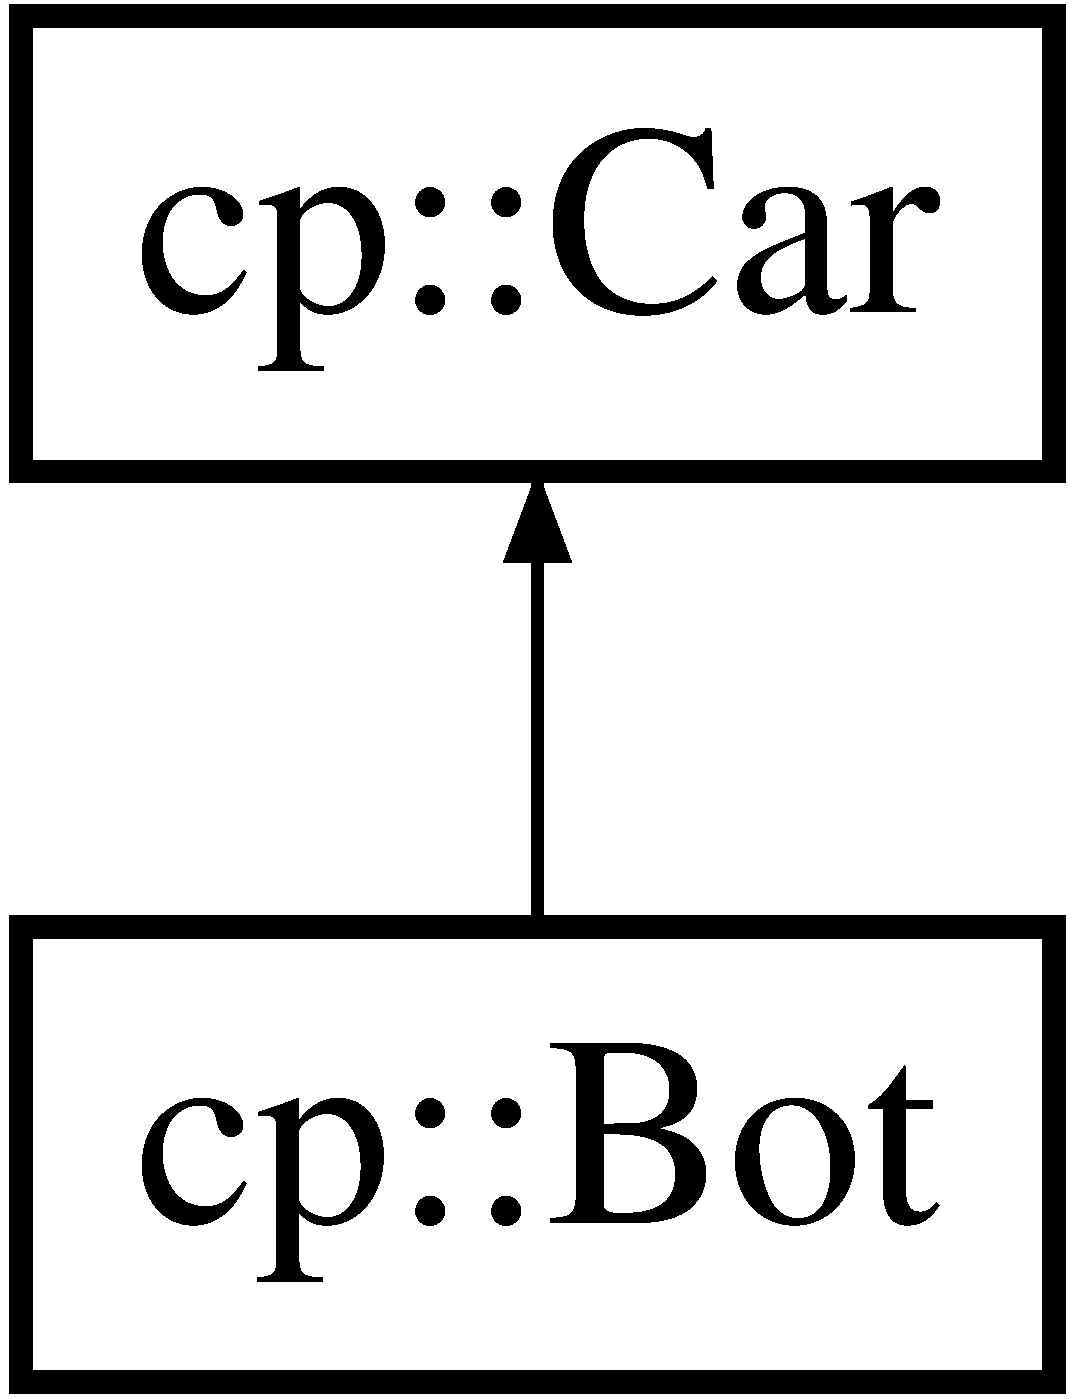
\includegraphics[height=2.000000cm]{classcp_1_1_bot}
\end{center}
\end{figure}
\subsection*{Public Types}
\begin{DoxyCompactItemize}
\item 
\mbox{\Hypertarget{classcp_1_1_bot_a0e9a97565604df18c5ea15e95cb626d9}\label{classcp_1_1_bot_a0e9a97565604df18c5ea15e95cb626d9}} 
using {\bfseries input\+\_\+type} = std\+::vector$<$ bool $>$
\end{DoxyCompactItemize}
\subsection*{Public Member Functions}
\begin{DoxyCompactItemize}
\item 
\mbox{\Hypertarget{classcp_1_1_bot_a206a47f38ff4d5ecacb085d669484c05}\label{classcp_1_1_bot_a206a47f38ff4d5ecacb085d669484c05}} 
{\bfseries Bot} (Game\+Data\+Ref \+\_\+data, int car\+\_\+num)
\item 
\mbox{\Hypertarget{classcp_1_1_bot_ae7218bd53d6ba9d1df22a45be4d353d5}\label{classcp_1_1_bot_ae7218bd53d6ba9d1df22a45be4d353d5}} 
void {\bfseries draw\+Sprite} (const \hyperlink{classcp_1_1_line}{Line} \&line)
\item 
\mbox{\Hypertarget{classcp_1_1_bot_aca81cf6805f57022a5182664d6eedb3e}\label{classcp_1_1_bot_aca81cf6805f57022a5182664d6eedb3e}} 
virtual void {\bfseries update\+\_\+car} (float dt, const std\+::vector$<$ \hyperlink{classcp_1_1_line}{Line} $>$ \&lines, float segL)
\item 
\mbox{\Hypertarget{classcp_1_1_bot_ab0b5d1af659659a34ad01ead5c183bbe}\label{classcp_1_1_bot_ab0b5d1af659659a34ad01ead5c183bbe}} 
void {\bfseries handle\+\_\+input} (input\+\_\+type mask, float dt)
\item 
\mbox{\Hypertarget{classcp_1_1_bot_afae88cef6bf398d58e1743188fa43837}\label{classcp_1_1_bot_afae88cef6bf398d58e1743188fa43837}} 
void {\bfseries handle\+\_\+input} ()
\end{DoxyCompactItemize}
\subsection*{Public Attributes}
\begin{DoxyCompactItemize}
\item 
\mbox{\Hypertarget{classcp_1_1_bot_a6aca543540b0f5cbb1f1b276c6ec65be}\label{classcp_1_1_bot_a6aca543540b0f5cbb1f1b276c6ec65be}} 
int {\bfseries img} = 1
\end{DoxyCompactItemize}


The documentation for this class was generated from the following files\+:\begin{DoxyCompactItemize}
\item 
include/\+Objects/Bot.\+hpp\item 
libs/Bot.\+cpp\end{DoxyCompactItemize}

\hypertarget{classcp_1_1_bullet}{}\section{cp\+:\+:Bullet Class Reference}
\label{classcp_1_1_bullet}\index{cp\+::\+Bullet@{cp\+::\+Bullet}}
Inheritance diagram for cp\+:\+:Bullet\+:\begin{figure}[H]
\begin{center}
\leavevmode
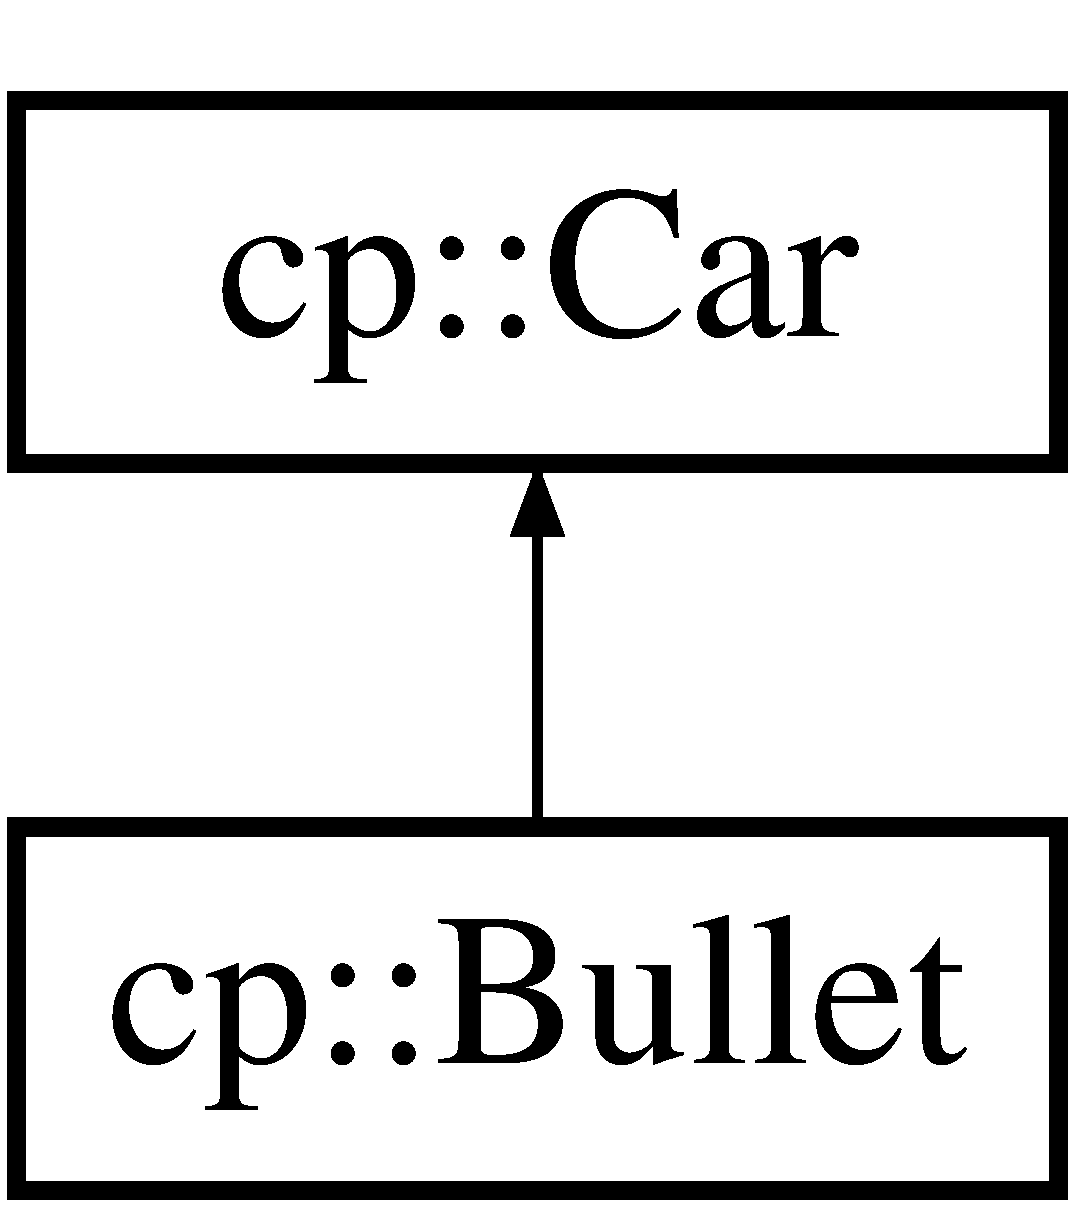
\includegraphics[height=2.000000cm]{classcp_1_1_bullet}
\end{center}
\end{figure}
\subsection*{Public Member Functions}
\begin{DoxyCompactItemize}
\item 
\mbox{\Hypertarget{classcp_1_1_bullet_af7953ddad292d8842e35bb194f5f725a}\label{classcp_1_1_bullet_af7953ddad292d8842e35bb194f5f725a}} 
{\bfseries Bullet} (Game\+Data\+Ref \+\_\+data, int car\+\_\+num)
\item 
\mbox{\Hypertarget{classcp_1_1_bullet_ae2cf83071115590f1a547cf7d3661f81}\label{classcp_1_1_bullet_ae2cf83071115590f1a547cf7d3661f81}} 
virtual void {\bfseries init} (sf\+::\+Vector3f pos)
\item 
\mbox{\Hypertarget{classcp_1_1_bullet_a6ec347cc013e55f5b533cccf142de133}\label{classcp_1_1_bullet_a6ec347cc013e55f5b533cccf142de133}} 
void {\bfseries draw\+Sprite} (const \hyperlink{classcp_1_1_line}{Line} \&line)
\item 
\mbox{\Hypertarget{classcp_1_1_bullet_a6710201781122f10b0451119dfc08521}\label{classcp_1_1_bullet_a6710201781122f10b0451119dfc08521}} 
virtual void {\bfseries update\+\_\+car} (float dt, const std\+::vector$<$ \hyperlink{classcp_1_1_line}{Line} $>$ \&lines, float segL)
\item 
\mbox{\Hypertarget{classcp_1_1_bullet_ad10ed3c00b3310951b622f0d180dbbc0}\label{classcp_1_1_bullet_ad10ed3c00b3310951b622f0d180dbbc0}} 
void {\bfseries handle\+\_\+input} ()
\end{DoxyCompactItemize}
\subsection*{Public Attributes}
\begin{DoxyCompactItemize}
\item 
\mbox{\Hypertarget{classcp_1_1_bullet_a508ef2a4895b5bd379f1cdbccbd5fab3}\label{classcp_1_1_bullet_a508ef2a4895b5bd379f1cdbccbd5fab3}} 
int {\bfseries frames} =0
\end{DoxyCompactItemize}


The documentation for this class was generated from the following files\+:\begin{DoxyCompactItemize}
\item 
include/\+Objects/Bullet.\+hpp\item 
libs/Bullet.\+cpp\end{DoxyCompactItemize}

\hypertarget{classcp_1_1_busted_state}{}\section{cp\+:\+:Busted\+State Class Reference}
\label{classcp_1_1_busted_state}\index{cp\+::\+Busted\+State@{cp\+::\+Busted\+State}}
Inheritance diagram for cp\+:\+:Busted\+State\+:\begin{figure}[H]
\begin{center}
\leavevmode
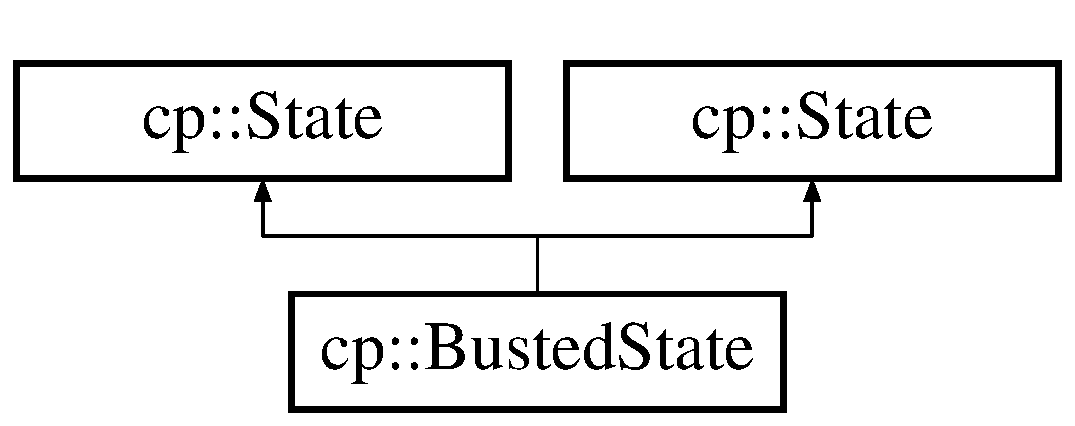
\includegraphics[height=2.000000cm]{classcp_1_1_busted_state}
\end{center}
\end{figure}
\subsection*{Public Member Functions}
\begin{DoxyCompactItemize}
\item 
\mbox{\Hypertarget{classcp_1_1_busted_state_a10df824b1aa48bab895bbe58eecdf5c5}\label{classcp_1_1_busted_state_a10df824b1aa48bab895bbe58eecdf5c5}} 
{\bfseries Busted\+State} (Game\+Data\+Ref \+\_\+data)
\item 
\mbox{\Hypertarget{classcp_1_1_busted_state_a9ac923c5b03d68e3d2f81c1f9a8b5e0b}\label{classcp_1_1_busted_state_a9ac923c5b03d68e3d2f81c1f9a8b5e0b}} 
void {\bfseries init} ()
\item 
\mbox{\Hypertarget{classcp_1_1_busted_state_a5ba8cb5f8e7991be6b6975a7c1086ac7}\label{classcp_1_1_busted_state_a5ba8cb5f8e7991be6b6975a7c1086ac7}} 
void {\bfseries draw} (float delta)
\item 
\mbox{\Hypertarget{classcp_1_1_busted_state_a4e6cae36e30f6e29c85550a75fba9b98}\label{classcp_1_1_busted_state_a4e6cae36e30f6e29c85550a75fba9b98}} 
void {\bfseries update} (float delta)
\item 
\mbox{\Hypertarget{classcp_1_1_busted_state_a6a834c039be196d923b575fbe270f09c}\label{classcp_1_1_busted_state_a6a834c039be196d923b575fbe270f09c}} 
void {\bfseries handle\+\_\+input} (float delta)
\item 
\mbox{\Hypertarget{classcp_1_1_busted_state_a10df824b1aa48bab895bbe58eecdf5c5}\label{classcp_1_1_busted_state_a10df824b1aa48bab895bbe58eecdf5c5}} 
{\bfseries Busted\+State} (Game\+Data\+Ref \+\_\+data)
\item 
\mbox{\Hypertarget{classcp_1_1_busted_state_a9ac923c5b03d68e3d2f81c1f9a8b5e0b}\label{classcp_1_1_busted_state_a9ac923c5b03d68e3d2f81c1f9a8b5e0b}} 
void {\bfseries init} ()
\item 
\mbox{\Hypertarget{classcp_1_1_busted_state_a5ba8cb5f8e7991be6b6975a7c1086ac7}\label{classcp_1_1_busted_state_a5ba8cb5f8e7991be6b6975a7c1086ac7}} 
void {\bfseries draw} (float delta)
\item 
\mbox{\Hypertarget{classcp_1_1_busted_state_a4e6cae36e30f6e29c85550a75fba9b98}\label{classcp_1_1_busted_state_a4e6cae36e30f6e29c85550a75fba9b98}} 
void {\bfseries update} (float delta)
\item 
\mbox{\Hypertarget{classcp_1_1_busted_state_a6a834c039be196d923b575fbe270f09c}\label{classcp_1_1_busted_state_a6a834c039be196d923b575fbe270f09c}} 
void {\bfseries handle\+\_\+input} (float delta)
\end{DoxyCompactItemize}


The documentation for this class was generated from the following files\+:\begin{DoxyCompactItemize}
\item 
include/Busted\+State.\+hpp\item 
libs/Busted\+State.\+cpp\end{DoxyCompactItemize}

\hypertarget{classcp_1_1_camera}{}\section{cp\+:\+:Camera Class Reference}
\label{classcp_1_1_camera}\index{cp\+::\+Camera@{cp\+::\+Camera}}
\subsection*{Public Member Functions}
\begin{DoxyCompactItemize}
\item 
\mbox{\Hypertarget{classcp_1_1_camera_af2cf800a9b18bbe6c07fb936b1b500e0}\label{classcp_1_1_camera_af2cf800a9b18bbe6c07fb936b1b500e0}} 
const sf\+::\+Vector3f \& {\bfseries get\+Position} () const
\item 
\mbox{\Hypertarget{classcp_1_1_camera_aedd15f99e37bd4a2290df292763f45e2}\label{classcp_1_1_camera_aedd15f99e37bd4a2290df292763f45e2}} 
const sf\+::\+Vector3f \& {\bfseries get\+Speed} () const
\item 
\mbox{\Hypertarget{classcp_1_1_camera_a8cf1b15d3424f94e0fb944c40415f245}\label{classcp_1_1_camera_a8cf1b15d3424f94e0fb944c40415f245}} 
void {\bfseries catch\+\_\+player} (const \hyperlink{classcp_1_1_car}{Car} \&player)
\item 
\mbox{\Hypertarget{classcp_1_1_camera_a000634184a814ee273ab48bb50096438}\label{classcp_1_1_camera_a000634184a814ee273ab48bb50096438}} 
float {\bfseries get\+CamD} () const
\item 
\mbox{\Hypertarget{classcp_1_1_camera_ac25389929c298ab44bec4b23c557ae44}\label{classcp_1_1_camera_ac25389929c298ab44bec4b23c557ae44}} 
void {\bfseries handle\+\_\+input} ()
\end{DoxyCompactItemize}
\subsection*{Public Attributes}
\begin{DoxyCompactItemize}
\item 
\mbox{\Hypertarget{classcp_1_1_camera_a6757f04379bd0a61dd20f1361685c5ef}\label{classcp_1_1_camera_a6757f04379bd0a61dd20f1361685c5ef}} 
std\+::thread\+::id {\bfseries id}
\item 
\mbox{\Hypertarget{classcp_1_1_camera_af65ba40e460d7fbfa946f8e8e0e08cab}\label{classcp_1_1_camera_af65ba40e460d7fbfa946f8e8e0e08cab}} 
sf\+::\+Vector3f {\bfseries e\+\_\+position} = sf\+::\+Vector3f(0, 1500, 0)
\end{DoxyCompactItemize}


The documentation for this class was generated from the following file\+:\begin{DoxyCompactItemize}
\item 
include/\+Objects/Camera.\+hpp\end{DoxyCompactItemize}

\hypertarget{classcp_1_1_car}{}\section{cp\+:\+:Car Class Reference}
\label{classcp_1_1_car}\index{cp\+::\+Car@{cp\+::\+Car}}
Inheritance diagram for cp\+:\+:Car\+:\begin{figure}[H]
\begin{center}
\leavevmode
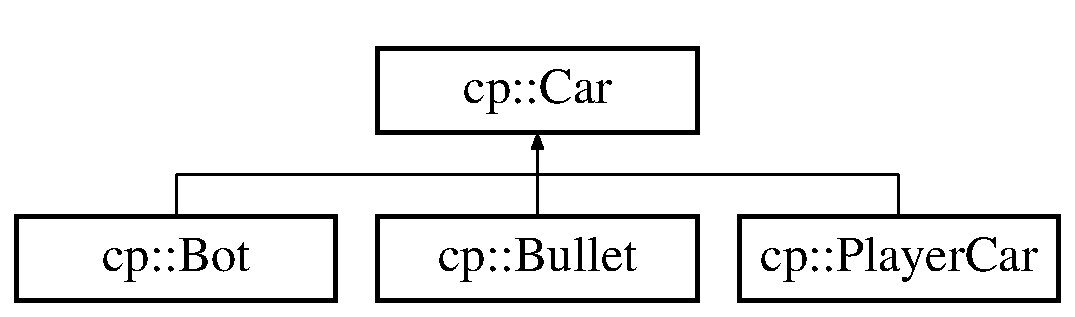
\includegraphics[height=2.000000cm]{classcp_1_1_car}
\end{center}
\end{figure}
\subsection*{Public Member Functions}
\begin{DoxyCompactItemize}
\item 
\mbox{\Hypertarget{classcp_1_1_car_a46616a5f3b166d287038bd112a2febf6}\label{classcp_1_1_car_a46616a5f3b166d287038bd112a2febf6}} 
{\bfseries Car} (Game\+Data\+Ref \+\_\+data, int car\+\_\+num)
\item 
\mbox{\Hypertarget{classcp_1_1_car_ad1ba1efee8393261c0df5665135a58f2}\label{classcp_1_1_car_ad1ba1efee8393261c0df5665135a58f2}} 
void {\bfseries draw\+\_\+car} ()
\item 
\mbox{\Hypertarget{classcp_1_1_car_a5314aafa100c37ff64a5f42e80421347}\label{classcp_1_1_car_a5314aafa100c37ff64a5f42e80421347}} 
virtual void {\bfseries init} (sf\+::\+Vector3f pos)
\item 
\mbox{\Hypertarget{classcp_1_1_car_aa9b3ace5ba3809f03b2d7ee2f692cb47}\label{classcp_1_1_car_aa9b3ace5ba3809f03b2d7ee2f692cb47}} 
void {\bfseries reset} ()
\item 
\mbox{\Hypertarget{classcp_1_1_car_a61f07d533f15f6241df726252ba634a5}\label{classcp_1_1_car_a61f07d533f15f6241df726252ba634a5}} 
virtual void {\bfseries update\+\_\+car} (float dt, const std\+::vector$<$ \hyperlink{classcp_1_1_line}{Line} $>$ \&lines, float segL)=0
\item 
\mbox{\Hypertarget{classcp_1_1_car_a1064f8e1d5f6ce98010ad7bdcd6f2648}\label{classcp_1_1_car_a1064f8e1d5f6ce98010ad7bdcd6f2648}} 
sf\+::\+Vector3f {\bfseries get\+Position} () const
\item 
\mbox{\Hypertarget{classcp_1_1_car_a57ea04dccfe2c989ff4de7071709c2fd}\label{classcp_1_1_car_a57ea04dccfe2c989ff4de7071709c2fd}} 
sf\+::\+Vector3f {\bfseries get\+Speed} () const
\item 
\mbox{\Hypertarget{classcp_1_1_car_a962c79b26ad0cee458e6fa1514161179}\label{classcp_1_1_car_a962c79b26ad0cee458e6fa1514161179}} 
void {\bfseries on\+Collision} ()
\end{DoxyCompactItemize}
\subsection*{Public Attributes}
\begin{DoxyCompactItemize}
\item 
\mbox{\Hypertarget{classcp_1_1_car_a9c0016df25c08d240b3d68df4b1a4d1e}\label{classcp_1_1_car_a9c0016df25c08d240b3d68df4b1a4d1e}} 
int {\bfseries car\+\_\+image\+\_\+num}
\item 
\mbox{\Hypertarget{classcp_1_1_car_abbcb271c156890f8edf120fbe13c9b55}\label{classcp_1_1_car_abbcb271c156890f8edf120fbe13c9b55}} 
bool {\bfseries l} = false
\item 
\mbox{\Hypertarget{classcp_1_1_car_a9532fda7653d8f7e564b4f1d2182680d}\label{classcp_1_1_car_a9532fda7653d8f7e564b4f1d2182680d}} 
bool {\bfseries r} = false
\item 
\mbox{\Hypertarget{classcp_1_1_car_a4be73a6980259975c78d02334a2ddcac}\label{classcp_1_1_car_a4be73a6980259975c78d02334a2ddcac}} 
sf\+::\+Sprite {\bfseries sprite}
\item 
\mbox{\Hypertarget{classcp_1_1_car_af6fc0e17ba216f124770ff2a54c637f5}\label{classcp_1_1_car_af6fc0e17ba216f124770ff2a54c637f5}} 
Game\+Data\+Ref {\bfseries data}
\item 
\mbox{\Hypertarget{classcp_1_1_car_a2e1c5e9f37be9bdd64a34767192ff2ed}\label{classcp_1_1_car_a2e1c5e9f37be9bdd64a34767192ff2ed}} 
sf\+::\+Vector3f {\bfseries e\+\_\+position}
\item 
\mbox{\Hypertarget{classcp_1_1_car_aca49ba4b184dd732e8191799af50ca36}\label{classcp_1_1_car_aca49ba4b184dd732e8191799af50ca36}} 
sf\+::\+Vector3f {\bfseries e\+\_\+speed}
\item 
\mbox{\Hypertarget{classcp_1_1_car_a9f4dcb1bf9ed9d74c1bee7f5069d3fdd}\label{classcp_1_1_car_a9f4dcb1bf9ed9d74c1bee7f5069d3fdd}} 
sf\+::\+Vector3f {\bfseries e\+\_\+acceleration}
\item 
\mbox{\Hypertarget{classcp_1_1_car_a3be0504b75d4ca80e50bc03160d3f94b}\label{classcp_1_1_car_a3be0504b75d4ca80e50bc03160d3f94b}} 
sf\+::\+Vector3f {\bfseries e\+\_\+decleration}
\item 
\mbox{\Hypertarget{classcp_1_1_car_ac4c002c522449207944a8783eb5781f5}\label{classcp_1_1_car_ac4c002c522449207944a8783eb5781f5}} 
sf\+::\+Vector3f {\bfseries e\+\_\+max\+\_\+speed}
\item 
\mbox{\Hypertarget{classcp_1_1_car_a52c4d6a9cc0923934e92c92e4fb98be3}\label{classcp_1_1_car_a52c4d6a9cc0923934e92c92e4fb98be3}} 
float {\bfseries centrifugal} = 0.\+5
\item 
\mbox{\Hypertarget{classcp_1_1_car_a4c9959533d302656a6b4a02f4a0c0cb1}\label{classcp_1_1_car_a4c9959533d302656a6b4a02f4a0c0cb1}} 
float {\bfseries car\+\_\+mass} =0
\item 
\mbox{\Hypertarget{classcp_1_1_car_a9cc4a38a4ff13fa7643947ca4f2c1776}\label{classcp_1_1_car_a9cc4a38a4ff13fa7643947ca4f2c1776}} 
float {\bfseries health} = 100
\item 
\mbox{\Hypertarget{classcp_1_1_car_a33253c0fb62bc8eb73de318bc7847106}\label{classcp_1_1_car_a33253c0fb62bc8eb73de318bc7847106}} 
bool {\bfseries in\+\_\+use} =false
\end{DoxyCompactItemize}


The documentation for this class was generated from the following files\+:\begin{DoxyCompactItemize}
\item 
include/\+Objects/Car.\+hpp\item 
libs/Car.\+cpp\end{DoxyCompactItemize}

\hypertarget{classcp_1_1_client}{}\section{cp\+:\+:Client Class Reference}
\label{classcp_1_1_client}\index{cp\+::\+Client@{cp\+::\+Client}}
\subsection*{Public Types}
\begin{DoxyCompactItemize}
\item 
\mbox{\Hypertarget{classcp_1_1_client_a1a4bc6b31cf85823c31298b70146069a}\label{classcp_1_1_client_a1a4bc6b31cf85823c31298b70146069a}} 
using {\bfseries ID} = long long int
\item 
\mbox{\Hypertarget{classcp_1_1_client_a7e69dcf4f9e235f0ef6e9b85f1f5e9fc}\label{classcp_1_1_client_a7e69dcf4f9e235f0ef6e9b85f1f5e9fc}} 
using {\bfseries IP} = std\+::string
\item 
\mbox{\Hypertarget{classcp_1_1_client_a2815b2c6eb61baa1b53994ca56aaaf3c}\label{classcp_1_1_client_a2815b2c6eb61baa1b53994ca56aaaf3c}} 
using {\bfseries key\+\_\+input\+\_\+type} = std\+::pair$<$ ID, std\+::vector$<$ bool $>$ $>$
\end{DoxyCompactItemize}
\subsection*{Public Member Functions}
\begin{DoxyCompactItemize}
\item 
\hyperlink{classcp_1_1_client_ae0c68ae53a2bb2ce6b2d90ee751ce2a2}{Client} (ID identity)
\begin{DoxyCompactList}\small\item\em Construct a new \hyperlink{classcp_1_1_client}{Client} object. \end{DoxyCompactList}\item 
sf\+::\+Tcp\+Socket \& \hyperlink{classcp_1_1_client_a00d100072786f290ef74aa13fa19eb4c}{get\+\_\+socket} ()
\begin{DoxyCompactList}\small\item\em Get the socket object. \end{DoxyCompactList}\item 
ID \hyperlink{classcp_1_1_client_af18deba2fb9aff79c9221ab4d89f4120}{get\+\_\+identity} () const
\begin{DoxyCompactList}\small\item\em Get the identity of the \hyperlink{classcp_1_1_client}{Client}. \end{DoxyCompactList}\item 
void \hyperlink{classcp_1_1_client_a6da5c65dc07b98f84b221c3a80e23c96}{connect\+\_\+to} (const std\+::string \&ip, int port)
\begin{DoxyCompactList}\small\item\em Utility function to connec to host. \end{DoxyCompactList}\item 
void \hyperlink{classcp_1_1_client_a8f0775eeb130ae6aa5cc67978b6e0ca5}{send\+\_\+packet} (sf\+::\+Packet \&packet)
\begin{DoxyCompactList}\small\item\em Utility to send packet over the network to the client connected to other end. \end{DoxyCompactList}\item 
void \hyperlink{classcp_1_1_client_a7b52fd5525cdb44e6238c617baa08a68}{recieve\+\_\+packet} (sf\+::\+Packet \&packet)
\begin{DoxyCompactList}\small\item\em Utility function to recieve a packet from other end. \end{DoxyCompactList}\item 
sf\+::\+Socket\+::\+Status \hyperlink{classcp_1_1_client_acbb62103eeab8e6bdf2bd978396b352d}{get\+Last\+Status} () const
\begin{DoxyCompactList}\small\item\em Get the Last Status object. \end{DoxyCompactList}\end{DoxyCompactItemize}
\subsection*{Friends}
\begin{DoxyCompactItemize}
\item 
\hyperlink{classcp_1_1_client}{Client} \& \hyperlink{classcp_1_1_client_a5be004df779610d45f3ab82b8d869d19}{operator$<$$<$} (\hyperlink{classcp_1_1_client}{Client} \&client, const \hyperlink{classcp_1_1_game_simulator_snap}{Game\+Simulator\+Snap} \&snap)
\begin{DoxyCompactList}\small\item\em Friend function for operator$<$$<$ overloaded for sending snap over the network. \end{DoxyCompactList}\item 
\hyperlink{classcp_1_1_client}{Client} \& \hyperlink{classcp_1_1_client_a5ad18fedde7ea3af7df0b681df49ab3d}{operator$>$$>$} (\hyperlink{classcp_1_1_client}{Client} \&client, key\+\_\+input\+\_\+type \&labelled\+\_\+input)
\begin{DoxyCompactList}\small\item\em Overloaded operator$>$$>$ to send labelled input over the network. \end{DoxyCompactList}\end{DoxyCompactItemize}


\subsection{Constructor \& Destructor Documentation}
\mbox{\Hypertarget{classcp_1_1_client_ae0c68ae53a2bb2ce6b2d90ee751ce2a2}\label{classcp_1_1_client_ae0c68ae53a2bb2ce6b2d90ee751ce2a2}} 
\index{cp\+::\+Client@{cp\+::\+Client}!Client@{Client}}
\index{Client@{Client}!cp\+::\+Client@{cp\+::\+Client}}
\subsubsection{\texorpdfstring{Client()}{Client()}}
{\footnotesize\ttfamily cp\+::\+Client\+::\+Client (\begin{DoxyParamCaption}\item[{ID}]{identity }\end{DoxyParamCaption})\hspace{0.3cm}{\ttfamily [inline]}}



Construct a new \hyperlink{classcp_1_1_client}{Client} object. 


\begin{DoxyParams}{Parameters}
{\em identity} & desired id of the client. \\
\hline
\end{DoxyParams}


\subsection{Member Function Documentation}
\mbox{\Hypertarget{classcp_1_1_client_a6da5c65dc07b98f84b221c3a80e23c96}\label{classcp_1_1_client_a6da5c65dc07b98f84b221c3a80e23c96}} 
\index{cp\+::\+Client@{cp\+::\+Client}!connect\+\_\+to@{connect\+\_\+to}}
\index{connect\+\_\+to@{connect\+\_\+to}!cp\+::\+Client@{cp\+::\+Client}}
\subsubsection{\texorpdfstring{connect\+\_\+to()}{connect\_to()}}
{\footnotesize\ttfamily void cp\+::\+Client\+::connect\+\_\+to (\begin{DoxyParamCaption}\item[{const std\+::string \&}]{ip,  }\item[{int}]{port }\end{DoxyParamCaption})\hspace{0.3cm}{\ttfamily [inline]}}



Utility function to connec to host. 


\begin{DoxyParams}{Parameters}
{\em ip} & IP of the host. \\
\hline
{\em port} & P\+O\+RT number of the host. \\
\hline
\end{DoxyParams}
\mbox{\Hypertarget{classcp_1_1_client_af18deba2fb9aff79c9221ab4d89f4120}\label{classcp_1_1_client_af18deba2fb9aff79c9221ab4d89f4120}} 
\index{cp\+::\+Client@{cp\+::\+Client}!get\+\_\+identity@{get\+\_\+identity}}
\index{get\+\_\+identity@{get\+\_\+identity}!cp\+::\+Client@{cp\+::\+Client}}
\subsubsection{\texorpdfstring{get\+\_\+identity()}{get\_identity()}}
{\footnotesize\ttfamily ID cp\+::\+Client\+::get\+\_\+identity (\begin{DoxyParamCaption}{ }\end{DoxyParamCaption}) const\hspace{0.3cm}{\ttfamily [inline]}}



Get the identity of the \hyperlink{classcp_1_1_client}{Client}. 

\begin{DoxyReturn}{Returns}
ID id of the client. 
\end{DoxyReturn}
\mbox{\Hypertarget{classcp_1_1_client_a00d100072786f290ef74aa13fa19eb4c}\label{classcp_1_1_client_a00d100072786f290ef74aa13fa19eb4c}} 
\index{cp\+::\+Client@{cp\+::\+Client}!get\+\_\+socket@{get\+\_\+socket}}
\index{get\+\_\+socket@{get\+\_\+socket}!cp\+::\+Client@{cp\+::\+Client}}
\subsubsection{\texorpdfstring{get\+\_\+socket()}{get\_socket()}}
{\footnotesize\ttfamily sf\+::\+Tcp\+Socket\& cp\+::\+Client\+::get\+\_\+socket (\begin{DoxyParamCaption}{ }\end{DoxyParamCaption})\hspace{0.3cm}{\ttfamily [inline]}}



Get the socket object. 

\begin{DoxyReturn}{Returns}
sf\+::\+Tcp\+Socket\& Internal Socket of the client. 
\end{DoxyReturn}
\mbox{\Hypertarget{classcp_1_1_client_acbb62103eeab8e6bdf2bd978396b352d}\label{classcp_1_1_client_acbb62103eeab8e6bdf2bd978396b352d}} 
\index{cp\+::\+Client@{cp\+::\+Client}!get\+Last\+Status@{get\+Last\+Status}}
\index{get\+Last\+Status@{get\+Last\+Status}!cp\+::\+Client@{cp\+::\+Client}}
\subsubsection{\texorpdfstring{get\+Last\+Status()}{getLastStatus()}}
{\footnotesize\ttfamily sf\+::\+Socket\+::\+Status cp\+::\+Client\+::get\+Last\+Status (\begin{DoxyParamCaption}{ }\end{DoxyParamCaption}) const\hspace{0.3cm}{\ttfamily [inline]}}



Get the Last Status object. 

\begin{DoxyReturn}{Returns}
sf\+::\+Socket\+::\+Status Returns the status of the last call to send/recieve. 
\end{DoxyReturn}
\mbox{\Hypertarget{classcp_1_1_client_a7b52fd5525cdb44e6238c617baa08a68}\label{classcp_1_1_client_a7b52fd5525cdb44e6238c617baa08a68}} 
\index{cp\+::\+Client@{cp\+::\+Client}!recieve\+\_\+packet@{recieve\+\_\+packet}}
\index{recieve\+\_\+packet@{recieve\+\_\+packet}!cp\+::\+Client@{cp\+::\+Client}}
\subsubsection{\texorpdfstring{recieve\+\_\+packet()}{recieve\_packet()}}
{\footnotesize\ttfamily void cp\+::\+Client\+::recieve\+\_\+packet (\begin{DoxyParamCaption}\item[{sf\+::\+Packet \&}]{packet }\end{DoxyParamCaption})\hspace{0.3cm}{\ttfamily [inline]}}



Utility function to recieve a packet from other end. 


\begin{DoxyParams}{Parameters}
{\em packet} & The packet that you want to recieve data into. \\
\hline
\end{DoxyParams}
\mbox{\Hypertarget{classcp_1_1_client_a8f0775eeb130ae6aa5cc67978b6e0ca5}\label{classcp_1_1_client_a8f0775eeb130ae6aa5cc67978b6e0ca5}} 
\index{cp\+::\+Client@{cp\+::\+Client}!send\+\_\+packet@{send\+\_\+packet}}
\index{send\+\_\+packet@{send\+\_\+packet}!cp\+::\+Client@{cp\+::\+Client}}
\subsubsection{\texorpdfstring{send\+\_\+packet()}{send\_packet()}}
{\footnotesize\ttfamily void cp\+::\+Client\+::send\+\_\+packet (\begin{DoxyParamCaption}\item[{sf\+::\+Packet \&}]{packet }\end{DoxyParamCaption})\hspace{0.3cm}{\ttfamily [inline]}}



Utility to send packet over the network to the client connected to other end. 


\begin{DoxyParams}{Parameters}
{\em packet} & The packet that you want to send . \\
\hline
\end{DoxyParams}


\subsection{Friends And Related Function Documentation}
\mbox{\Hypertarget{classcp_1_1_client_a5be004df779610d45f3ab82b8d869d19}\label{classcp_1_1_client_a5be004df779610d45f3ab82b8d869d19}} 
\index{cp\+::\+Client@{cp\+::\+Client}!operator$<$$<$@{operator$<$$<$}}
\index{operator$<$$<$@{operator$<$$<$}!cp\+::\+Client@{cp\+::\+Client}}
\subsubsection{\texorpdfstring{operator$<$$<$}{operator<<}}
{\footnotesize\ttfamily \hyperlink{classcp_1_1_client}{Client}\& operator$<$$<$ (\begin{DoxyParamCaption}\item[{\hyperlink{classcp_1_1_client}{Client} \&}]{client,  }\item[{const \hyperlink{classcp_1_1_game_simulator_snap}{Game\+Simulator\+Snap} \&}]{snap }\end{DoxyParamCaption})\hspace{0.3cm}{\ttfamily [friend]}}



Friend function for operator$<$$<$ overloaded for sending snap over the network. 


\begin{DoxyParams}{Parameters}
{\em client} & \hyperlink{classcp_1_1_client}{Client} that you want to send the snap to. \\
\hline
{\em snap} & The snap that you want to send. \\
\hline
\end{DoxyParams}
\begin{DoxyReturn}{Returns}
\hyperlink{classcp_1_1_client}{Client}\& Returns \hyperlink{classcp_1_1_client}{Client} object back. 
\end{DoxyReturn}
\mbox{\Hypertarget{classcp_1_1_client_a5ad18fedde7ea3af7df0b681df49ab3d}\label{classcp_1_1_client_a5ad18fedde7ea3af7df0b681df49ab3d}} 
\index{cp\+::\+Client@{cp\+::\+Client}!operator$>$$>$@{operator$>$$>$}}
\index{operator$>$$>$@{operator$>$$>$}!cp\+::\+Client@{cp\+::\+Client}}
\subsubsection{\texorpdfstring{operator$>$$>$}{operator>>}}
{\footnotesize\ttfamily \hyperlink{classcp_1_1_client}{Client}\& operator$>$$>$ (\begin{DoxyParamCaption}\item[{\hyperlink{classcp_1_1_client}{Client} \&}]{client,  }\item[{key\+\_\+input\+\_\+type \&}]{labelled\+\_\+input }\end{DoxyParamCaption})\hspace{0.3cm}{\ttfamily [friend]}}



Overloaded operator$>$$>$ to send labelled input over the network. 


\begin{DoxyParams}{Parameters}
{\em client} & The client object to which you want to send the labelled input \\
\hline
{\em labelled\+\_\+input} & The labelled input that you want to send. \\
\hline
\end{DoxyParams}
\begin{DoxyReturn}{Returns}
\hyperlink{classcp_1_1_client}{Client}\& Returns back the \hyperlink{classcp_1_1_client}{Client} Reference. 
\end{DoxyReturn}


The documentation for this class was generated from the following file\+:\begin{DoxyCompactItemize}
\item 
include/\+Network/\hyperlink{_client_8hpp}{Client.\+hpp}\end{DoxyCompactItemize}

\hypertarget{classcp_1_1_client_room}{}\section{cp\+:\+:Client\+Room Class Reference}
\label{classcp_1_1_client_room}\index{cp\+::\+Client\+Room@{cp\+::\+Client\+Room}}
Inheritance diagram for cp\+:\+:Client\+Room\+:\begin{figure}[H]
\begin{center}
\leavevmode
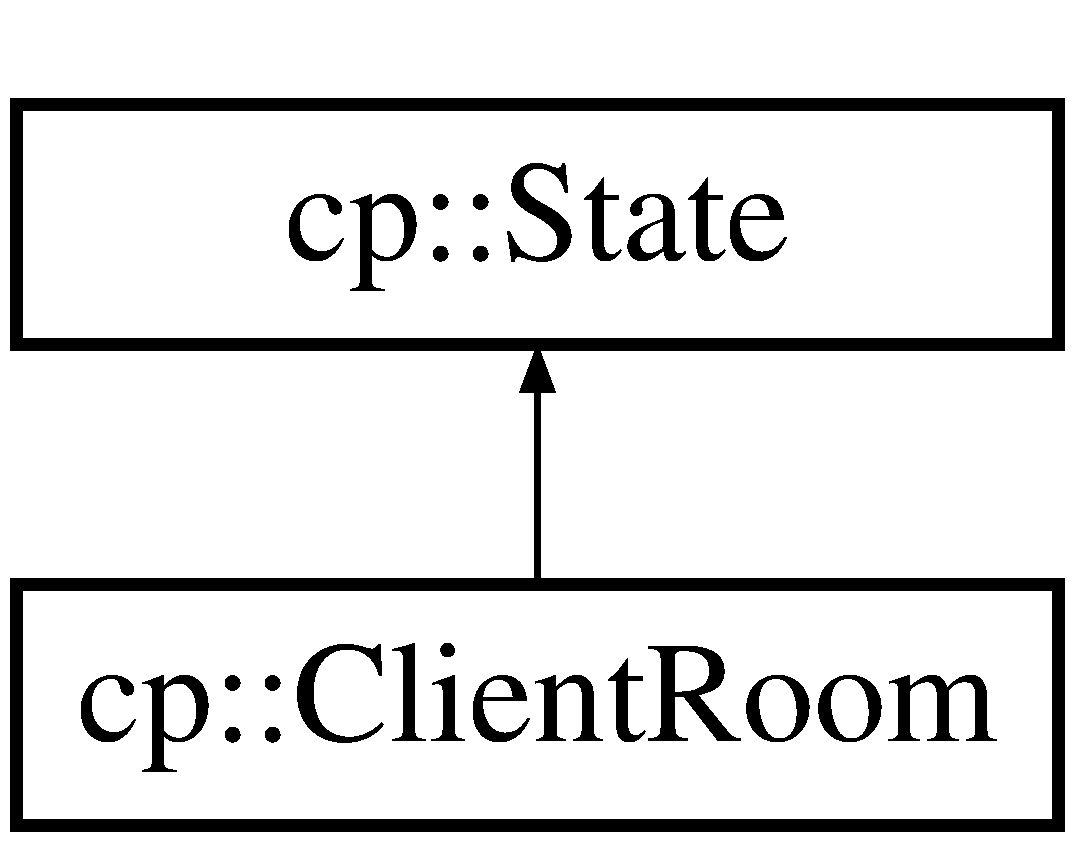
\includegraphics[height=2.000000cm]{classcp_1_1_client_room}
\end{center}
\end{figure}
\subsection*{Public Member Functions}
\begin{DoxyCompactItemize}
\item 
\mbox{\Hypertarget{classcp_1_1_client_room_a8e636ababbdc41c50f486d37af2b64d5}\label{classcp_1_1_client_room_a8e636ababbdc41c50f486d37af2b64d5}} 
{\bfseries Client\+Room} (Game\+Data\+Ref \+\_\+data)
\item 
\mbox{\Hypertarget{classcp_1_1_client_room_a9fa2892e03ca5eb0cce9221e83320058}\label{classcp_1_1_client_room_a9fa2892e03ca5eb0cce9221e83320058}} 
void \hyperlink{classcp_1_1_client_room_a9fa2892e03ca5eb0cce9221e83320058}{init} ()
\begin{DoxyCompactList}\small\item\em Initializing the \hyperlink{classcp_1_1_client_room}{Client\+Room} components. \end{DoxyCompactList}\item 
void \hyperlink{classcp_1_1_client_room_a8e0de6eeab8147b7d918b11c2eeccecf}{handle\+\_\+input} (float delta)
\begin{DoxyCompactList}\small\item\em T\+His function provides the interface to handle\+\_\+input in \hyperlink{classcp_1_1_client_room}{Client\+Room}. \end{DoxyCompactList}\item 
void \hyperlink{classcp_1_1_client_room_a09987dd7d61af43329b63a8ba9e3df69}{update} (float delta)
\begin{DoxyCompactList}\small\item\em Provides an interface to update the \hyperlink{classcp_1_1_client_room}{Client\+Room}. \end{DoxyCompactList}\item 
void \hyperlink{classcp_1_1_client_room_a9c8ff4227d9fa5e35511c756ddaafc83}{draw} (float delta)
\begin{DoxyCompactList}\small\item\em Draw the components on the screen. \end{DoxyCompactList}\item 
\mbox{\Hypertarget{classcp_1_1_client_room_a073602b25e64da5644a0deb3ecbe1146}\label{classcp_1_1_client_room_a073602b25e64da5644a0deb3ecbe1146}} 
void \hyperlink{classcp_1_1_client_room_a073602b25e64da5644a0deb3ecbe1146}{get\+\_\+notifications} ()
\begin{DoxyCompactList}\small\item\em Get the notifications from the server. \end{DoxyCompactList}\item 
\mbox{\Hypertarget{classcp_1_1_client_room_abea3f2a34f619f4b2637b1486a809081}\label{classcp_1_1_client_room_abea3f2a34f619f4b2637b1486a809081}} 
void \hyperlink{classcp_1_1_client_room_abea3f2a34f619f4b2637b1486a809081}{use\+\_\+notification} ()
\begin{DoxyCompactList}\small\item\em Utility function to use\+\_\+recieved notification. \end{DoxyCompactList}\end{DoxyCompactItemize}


\subsection{Member Function Documentation}
\mbox{\Hypertarget{classcp_1_1_client_room_a9c8ff4227d9fa5e35511c756ddaafc83}\label{classcp_1_1_client_room_a9c8ff4227d9fa5e35511c756ddaafc83}} 
\index{cp\+::\+Client\+Room@{cp\+::\+Client\+Room}!draw@{draw}}
\index{draw@{draw}!cp\+::\+Client\+Room@{cp\+::\+Client\+Room}}
\subsubsection{\texorpdfstring{draw()}{draw()}}
{\footnotesize\ttfamily void cp\+::\+Client\+Room\+::draw (\begin{DoxyParamCaption}\item[{float}]{delta }\end{DoxyParamCaption})\hspace{0.3cm}{\ttfamily [inline]}, {\ttfamily [virtual]}}



Draw the components on the screen. 


\begin{DoxyParams}{Parameters}
{\em delta} & \\
\hline
\end{DoxyParams}


Implements \hyperlink{classcp_1_1_state}{cp\+::\+State}.

\mbox{\Hypertarget{classcp_1_1_client_room_a8e0de6eeab8147b7d918b11c2eeccecf}\label{classcp_1_1_client_room_a8e0de6eeab8147b7d918b11c2eeccecf}} 
\index{cp\+::\+Client\+Room@{cp\+::\+Client\+Room}!handle\+\_\+input@{handle\+\_\+input}}
\index{handle\+\_\+input@{handle\+\_\+input}!cp\+::\+Client\+Room@{cp\+::\+Client\+Room}}
\subsubsection{\texorpdfstring{handle\+\_\+input()}{handle\_input()}}
{\footnotesize\ttfamily void cp\+::\+Client\+Room\+::handle\+\_\+input (\begin{DoxyParamCaption}\item[{float}]{delta }\end{DoxyParamCaption})\hspace{0.3cm}{\ttfamily [inline]}, {\ttfamily [virtual]}}



T\+His function provides the interface to handle\+\_\+input in \hyperlink{classcp_1_1_client_room}{Client\+Room}. 


\begin{DoxyParams}{Parameters}
{\em delta} & T\+Ime difference between two handle\+\_\+input calls. \\
\hline
\end{DoxyParams}


Implements \hyperlink{classcp_1_1_state}{cp\+::\+State}.

\mbox{\Hypertarget{classcp_1_1_client_room_a09987dd7d61af43329b63a8ba9e3df69}\label{classcp_1_1_client_room_a09987dd7d61af43329b63a8ba9e3df69}} 
\index{cp\+::\+Client\+Room@{cp\+::\+Client\+Room}!update@{update}}
\index{update@{update}!cp\+::\+Client\+Room@{cp\+::\+Client\+Room}}
\subsubsection{\texorpdfstring{update()}{update()}}
{\footnotesize\ttfamily void cp\+::\+Client\+Room\+::update (\begin{DoxyParamCaption}\item[{float}]{delta }\end{DoxyParamCaption})\hspace{0.3cm}{\ttfamily [inline]}, {\ttfamily [virtual]}}



Provides an interface to update the \hyperlink{classcp_1_1_client_room}{Client\+Room}. 


\begin{DoxyParams}{Parameters}
{\em delta} & T\+Ime difference between two update calls \\
\hline
\end{DoxyParams}


Implements \hyperlink{classcp_1_1_state}{cp\+::\+State}.



The documentation for this class was generated from the following file\+:\begin{DoxyCompactItemize}
\item 
include/\+Network/\hyperlink{_client_room_8hpp}{Client\+Room.\+hpp}\end{DoxyCompactItemize}

\hypertarget{classcp_1_1_client_state}{}\section{cp\+:\+:Client\+State Class Reference}
\label{classcp_1_1_client_state}\index{cp\+::\+Client\+State@{cp\+::\+Client\+State}}
Inheritance diagram for cp\+:\+:Client\+State\+:\begin{figure}[H]
\begin{center}
\leavevmode
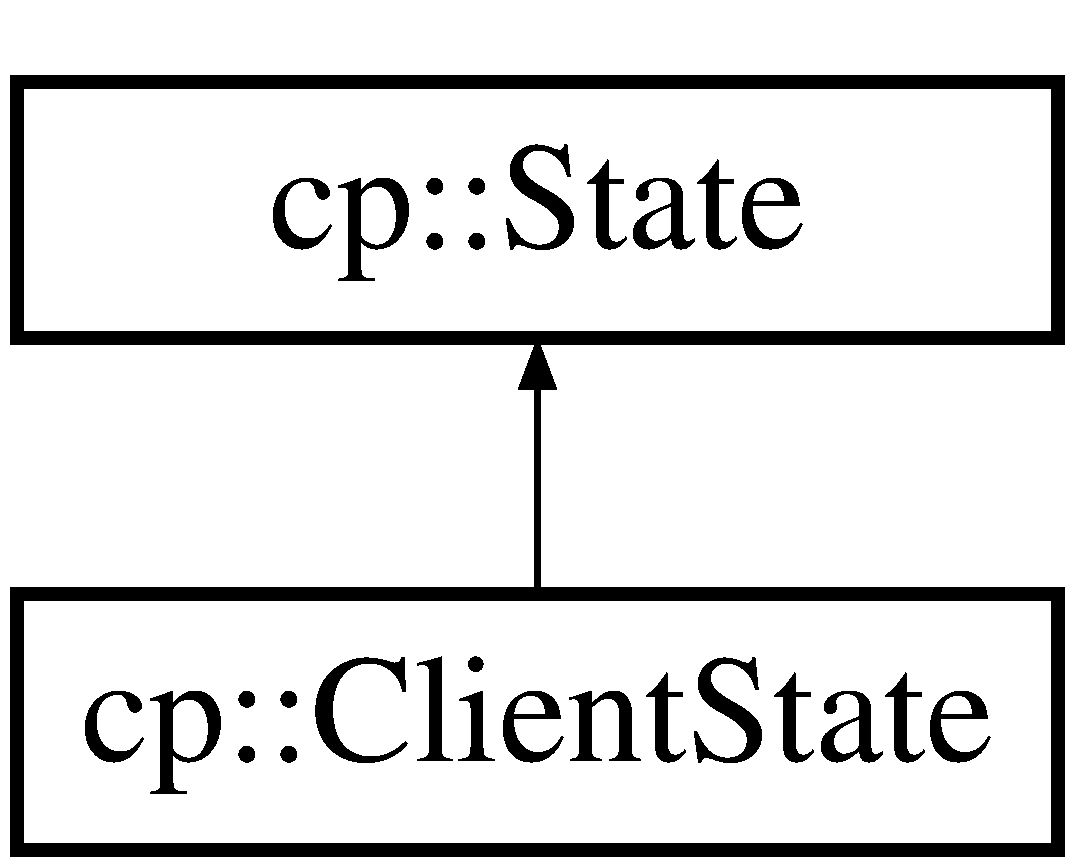
\includegraphics[height=2.000000cm]{classcp_1_1_client_state}
\end{center}
\end{figure}
\subsection*{Public Member Functions}
\begin{DoxyCompactItemize}
\item 
\mbox{\Hypertarget{classcp_1_1_client_state_a1bc5e08dad0a0a3db874f8770f70eee0}\label{classcp_1_1_client_state_a1bc5e08dad0a0a3db874f8770f70eee0}} 
{\bfseries Client\+State} (Game\+Data\+Ref \+\_\+data, Server\+\_\+ptr server, int unique\+\_\+id)
\item 
\mbox{\Hypertarget{classcp_1_1_client_state_a51770935e2bb3d5b3da9172a7bb7f254}\label{classcp_1_1_client_state_a51770935e2bb3d5b3da9172a7bb7f254}} 
virtual void {\bfseries init} ()
\item 
\mbox{\Hypertarget{classcp_1_1_client_state_a06e11fa2d76322fbec09da8cf10b609e}\label{classcp_1_1_client_state_a06e11fa2d76322fbec09da8cf10b609e}} 
virtual void {\bfseries handle\+\_\+input} (float delta)
\item 
\mbox{\Hypertarget{classcp_1_1_client_state_abb22a00f3cafa3585d737ca22e080e62}\label{classcp_1_1_client_state_abb22a00f3cafa3585d737ca22e080e62}} 
virtual void {\bfseries update} (float delta)
\item 
\mbox{\Hypertarget{classcp_1_1_client_state_a1846e3b9d306d00591550f1eb310ea90}\label{classcp_1_1_client_state_a1846e3b9d306d00591550f1eb310ea90}} 
virtual void {\bfseries draw} (float delta)
\item 
\mbox{\Hypertarget{classcp_1_1_client_state_a5ecebcbb46e52b89da6c76de4012e180}\label{classcp_1_1_client_state_a5ecebcbb46e52b89da6c76de4012e180}} 
virtual void {\bfseries pause} ()
\item 
\mbox{\Hypertarget{classcp_1_1_client_state_a19eaed84d6ea633c2878648f0f4814c8}\label{classcp_1_1_client_state_a19eaed84d6ea633c2878648f0f4814c8}} 
virtual void {\bfseries resume} ()
\end{DoxyCompactItemize}


The documentation for this class was generated from the following files\+:\begin{DoxyCompactItemize}
\item 
include/\+States/\hyperlink{_client_state_8hpp}{Client\+State.\+hpp}\item 
libs/Client\+State.\+cpp\end{DoxyCompactItemize}

\hypertarget{classcp_1_1_collision}{}\section{cp\+:\+:Collision Class Reference}
\label{classcp_1_1_collision}\index{cp\+::\+Collision@{cp\+::\+Collision}}
\subsection*{Public Member Functions}
\begin{DoxyCompactItemize}
\item 
\mbox{\Hypertarget{classcp_1_1_collision_a71a52f984bb843a3dd1aa0f486c359ea}\label{classcp_1_1_collision_a71a52f984bb843a3dd1aa0f486c359ea}} 
bool {\bfseries handle\+\_\+collision} (\hyperlink{classcp_1_1_car}{Car} \&car1, \hyperlink{classcp_1_1_car}{Car} \&car2, \hyperlink{classcp_1_1_game_map}{Game\+Map} \&map, float cor)
\end{DoxyCompactItemize}
\subsection*{Static Public Member Functions}
\begin{DoxyCompactItemize}
\item 
\mbox{\Hypertarget{classcp_1_1_collision_a045cd52fd5e25e035426ffea327f8ccb}\label{classcp_1_1_collision_a045cd52fd5e25e035426ffea327f8ccb}} 
static void {\bfseries simulate\+\_\+physics} (std\+::vector$<$ \hyperlink{classcp_1_1_car}{Car} $\ast$$>$ \&entities, \hyperlink{classcp_1_1_game_map}{Game\+Map} \&map)
\item 
\mbox{\Hypertarget{classcp_1_1_collision_a4a5156d0b8bece699830bb72920af45b}\label{classcp_1_1_collision_a4a5156d0b8bece699830bb72920af45b}} 
static void {\bfseries single\+\_\+entity\+\_\+check} (std\+::vector$<$ \hyperlink{classcp_1_1_car}{Car} $\ast$$>$ $\ast$entites\+\_\+ptr, int index, \hyperlink{classcp_1_1_game_map}{Game\+Map} $\ast$map\+\_\+ptr, std\+::mutex $\ast$mutex\+\_\+arr)
\item 
\mbox{\Hypertarget{classcp_1_1_collision_a8e1ec98476f6edd03df2eb27154c37ed}\label{classcp_1_1_collision_a8e1ec98476f6edd03df2eb27154c37ed}} 
static void {\bfseries handle\+\_\+collision} (\hyperlink{classcp_1_1_car}{Car} \&car1, \hyperlink{classcp_1_1_car}{Car} \&car2, \hyperlink{classcp_1_1_game_map}{Game\+Map} \&map)
\item 
\mbox{\Hypertarget{classcp_1_1_collision_a112e3aef8a60a0de8ca616f626023356}\label{classcp_1_1_collision_a112e3aef8a60a0de8ca616f626023356}} 
static void {\bfseries cover\+\_\+collided} (\hyperlink{classcp_1_1_car}{Car} \&car1, \hyperlink{classcp_1_1_car}{Car} \&car2, int diff, float cor)
\item 
\mbox{\Hypertarget{classcp_1_1_collision_a54f01c33786e0cf45fc7e58ac12c5e73}\label{classcp_1_1_collision_a54f01c33786e0cf45fc7e58ac12c5e73}} 
static bool {\bfseries detect\+\_\+collision} (const sf\+::\+Sprite \&s1, const sf\+::\+Sprite \&s2)
\end{DoxyCompactItemize}


The documentation for this class was generated from the following file\+:\begin{DoxyCompactItemize}
\item 
include/\+Physics/Collision.\+hpp\end{DoxyCompactItemize}

\hypertarget{classcp_1_1entity__info}{}\section{cp\+:\+:entity\+\_\+info Class Reference}
\label{classcp_1_1entity__info}\index{cp\+::entity\+\_\+info@{cp\+::entity\+\_\+info}}
\subsection*{Public Member Functions}
\begin{DoxyCompactItemize}
\item 
\mbox{\Hypertarget{classcp_1_1entity__info_a6c2b40ed8186772e704d4450681423ee}\label{classcp_1_1entity__info_a6c2b40ed8186772e704d4450681423ee}} 
{\bfseries entity\+\_\+info} (\hyperlink{classcp_1_1_player_car}{cp\+::\+Player\+Car} \&car)
\end{DoxyCompactItemize}
\subsection*{Friends}
\begin{DoxyCompactItemize}
\item 
\mbox{\Hypertarget{classcp_1_1entity__info_a5914b299fccea3f3c5ae2224cd4e2b3e}\label{classcp_1_1entity__info_a5914b299fccea3f3c5ae2224cd4e2b3e}} 
class {\bfseries Game\+Simulator}
\item 
\mbox{\Hypertarget{classcp_1_1entity__info_a64f8eecccbf7fd64b91d6b9c08c44c3e}\label{classcp_1_1entity__info_a64f8eecccbf7fd64b91d6b9c08c44c3e}} 
std\+::ofstream \& {\bfseries operator$<$$<$} (std\+::ofstream \&fout, const \hyperlink{classcp_1_1entity__info}{entity\+\_\+info} \&entity\+\_\+i)
\item 
\mbox{\Hypertarget{classcp_1_1entity__info_aa2ff1395cb67fc5d9016f5d1cb3019fe}\label{classcp_1_1entity__info_aa2ff1395cb67fc5d9016f5d1cb3019fe}} 
sf\+::\+Packet \& {\bfseries operator$<$$<$} (sf\+::\+Packet \&fout, const \hyperlink{classcp_1_1entity__info}{entity\+\_\+info} \&entity\+\_\+i)
\item 
\mbox{\Hypertarget{classcp_1_1entity__info_a7fbbc9d456cf16707aa9ad5839d87f15}\label{classcp_1_1entity__info_a7fbbc9d456cf16707aa9ad5839d87f15}} 
sf\+::\+Packet \& {\bfseries operator$>$$>$} (sf\+::\+Packet \&fin, \hyperlink{classcp_1_1entity__info}{entity\+\_\+info} \&entity\+\_\+i)
\end{DoxyCompactItemize}


The documentation for this class was generated from the following file\+:\begin{DoxyCompactItemize}
\item 
include/\+States/\hyperlink{_game_simulator_8hpp}{Game\+Simulator.\+hpp}\end{DoxyCompactItemize}

\hypertarget{classcp_1_1_game}{}\section{cp\+:\+:Game Class Reference}
\label{classcp_1_1_game}\index{cp\+::\+Game@{cp\+::\+Game}}
\subsection*{Public Member Functions}
\begin{DoxyCompactItemize}
\item 
\hyperlink{classcp_1_1_game_a3ae35e3d273bca248b415b9acb5b2010}{Game} (int width, int height, std\+::string title)
\begin{DoxyCompactList}\small\item\em Construct a new \hyperlink{classcp_1_1_game}{Game}\+:\+: \hyperlink{classcp_1_1_game}{Game} object. \end{DoxyCompactList}\item 
\mbox{\Hypertarget{classcp_1_1_game_a1c1387e83a2325e45cbf2099c430c502}\label{classcp_1_1_game_a1c1387e83a2325e45cbf2099c430c502}} 
\hyperlink{classcp_1_1_game_a1c1387e83a2325e45cbf2099c430c502}{$\sim$\+Game} ()
\begin{DoxyCompactList}\small\item\em Destroy the \hyperlink{classcp_1_1_game}{Game}\+:\+: \hyperlink{classcp_1_1_game}{Game} object. \end{DoxyCompactList}\end{DoxyCompactItemize}


\subsection{Constructor \& Destructor Documentation}
\mbox{\Hypertarget{classcp_1_1_game_a3ae35e3d273bca248b415b9acb5b2010}\label{classcp_1_1_game_a3ae35e3d273bca248b415b9acb5b2010}} 
\index{cp\+::\+Game@{cp\+::\+Game}!Game@{Game}}
\index{Game@{Game}!cp\+::\+Game@{cp\+::\+Game}}
\subsubsection{\texorpdfstring{Game()}{Game()}}
{\footnotesize\ttfamily cp\+::\+Game\+::\+Game (\begin{DoxyParamCaption}\item[{int}]{width,  }\item[{int}]{height,  }\item[{std\+::string}]{title }\end{DoxyParamCaption})}



Construct a new \hyperlink{classcp_1_1_game}{Game}\+:\+: \hyperlink{classcp_1_1_game}{Game} object. 


\begin{DoxyParams}{Parameters}
{\em width} & Width of the screen requested. \\
\hline
{\em height} & Height of the screen requested. \\
\hline
{\em title} & Title of the game screen. \\
\hline
\end{DoxyParams}


The documentation for this class was generated from the following files\+:\begin{DoxyCompactItemize}
\item 
include/Game.\+hpp\item 
libs/\hyperlink{_game_8cpp}{Game.\+cpp}\end{DoxyCompactItemize}

\hypertarget{structcp_1_1_game_data}{}\section{cp\+:\+:Game\+Data Struct Reference}
\label{structcp_1_1_game_data}\index{cp\+::\+Game\+Data@{cp\+::\+Game\+Data}}
\subsection*{Public Attributes}
\begin{DoxyCompactItemize}
\item 
\mbox{\Hypertarget{structcp_1_1_game_data_a6a80ac77dcf3186e54f672c1b14bdb41}\label{structcp_1_1_game_data_a6a80ac77dcf3186e54f672c1b14bdb41}} 
\hyperlink{classcp_1_1_state_machine}{State\+Machine} {\bfseries machine}
\item 
\mbox{\Hypertarget{structcp_1_1_game_data_a169d50257512a60497baf9f33471e4e7}\label{structcp_1_1_game_data_a169d50257512a60497baf9f33471e4e7}} 
sf\+::\+Render\+Window {\bfseries window}
\item 
\mbox{\Hypertarget{structcp_1_1_game_data_acf5734cc278e26e778d2bd47ea1317a4}\label{structcp_1_1_game_data_acf5734cc278e26e778d2bd47ea1317a4}} 
\hyperlink{classcp_1_1_asset_manager}{Asset\+Manager} {\bfseries assets}
\item 
\mbox{\Hypertarget{structcp_1_1_game_data_ab43a0b7f11ee1c4a651e11b89450c092}\label{structcp_1_1_game_data_ab43a0b7f11ee1c4a651e11b89450c092}} 
\hyperlink{classcp_1_1_input_manager}{Input\+Manager} {\bfseries input}
\item 
\mbox{\Hypertarget{structcp_1_1_game_data_ac68bb9af43fdfb2e455ca1cebd209eb5}\label{structcp_1_1_game_data_ac68bb9af43fdfb2e455ca1cebd209eb5}} 
\hyperlink{classcp_1_1_network_manager}{Network\+Manager} {\bfseries Nmanager}
\end{DoxyCompactItemize}


The documentation for this struct was generated from the following file\+:\begin{DoxyCompactItemize}
\item 
include/Game.\+hpp\end{DoxyCompactItemize}

\hypertarget{classcp_1_1_game_map}{}\section{cp\+:\+:Game\+Map Class Reference}
\label{classcp_1_1_game_map}\index{cp\+::\+Game\+Map@{cp\+::\+Game\+Map}}
\subsection*{Public Member Functions}
\begin{DoxyCompactItemize}
\item 
\mbox{\Hypertarget{classcp_1_1_game_map_a2d0def33bf9ef663f32d9abf7aca1844}\label{classcp_1_1_game_map_a2d0def33bf9ef663f32d9abf7aca1844}} 
{\bfseries Game\+Map} (Game\+Data\+Ref \+\_\+data)
\item 
\mbox{\Hypertarget{classcp_1_1_game_map_ad32e7dc2c373891d2b23be9d82298843}\label{classcp_1_1_game_map_ad32e7dc2c373891d2b23be9d82298843}} 
void {\bfseries init} ()
\item 
\mbox{\Hypertarget{classcp_1_1_game_map_a2e6704dd56becb268b447899dd325004}\label{classcp_1_1_game_map_a2e6704dd56becb268b447899dd325004}} 
void {\bfseries draw\+\_\+quad} (sf\+::\+Color c, int x1, int y1, int w1, int x2, int y2, int w2)
\item 
\mbox{\Hypertarget{classcp_1_1_game_map_a789a1f584569d46ade271dcbc729e0ae}\label{classcp_1_1_game_map_a789a1f584569d46ade271dcbc729e0ae}} 
void {\bfseries update} (float delta)
\item 
\mbox{\Hypertarget{classcp_1_1_game_map_a549c0c56f71a0dac1569064c9619b6ef}\label{classcp_1_1_game_map_a549c0c56f71a0dac1569064c9619b6ef}} 
void {\bfseries project} (\hyperlink{classcp_1_1_line}{Line} \&line, float camX, float camY, float camZ, float camD)
\item 
\mbox{\Hypertarget{classcp_1_1_game_map_a01e91f2a91d334c247e98eb9a1dc2cd9}\label{classcp_1_1_game_map_a01e91f2a91d334c247e98eb9a1dc2cd9}} 
void {\bfseries draw} (int count, const \hyperlink{classcp_1_1_camera}{Camera} \&main\+\_\+camera)
\item 
\mbox{\Hypertarget{classcp_1_1_game_map_a710565389773b9cc81645195bd835a1c}\label{classcp_1_1_game_map_a710565389773b9cc81645195bd835a1c}} 
void {\bfseries draw\+Sprite} (const \hyperlink{classcp_1_1_line}{Line} \&line)
\item 
\mbox{\Hypertarget{classcp_1_1_game_map_a7a191dba96e48afa77801cd76ffc601e}\label{classcp_1_1_game_map_a7a191dba96e48afa77801cd76ffc601e}} 
int {\bfseries get\+\_\+grid\+\_\+index} (float distance)
\item 
\mbox{\Hypertarget{classcp_1_1_game_map_a2bf537aba9c69a5916fd764afb7200a8}\label{classcp_1_1_game_map_a2bf537aba9c69a5916fd764afb7200a8}} 
void {\bfseries bound\+\_\+entity} (\hyperlink{classcp_1_1_car}{cp\+::\+Car} \&car)
\item 
\mbox{\Hypertarget{classcp_1_1_game_map_a0909cc97e391b711c7770497dffc97d3}\label{classcp_1_1_game_map_a0909cc97e391b711c7770497dffc97d3}} 
void {\bfseries bound\+\_\+entity} (\hyperlink{classcp_1_1_camera}{Camera} \&camera)
\item 
\mbox{\Hypertarget{classcp_1_1_game_map_a15e718a61f5244d39e38d425abcfef2c}\label{classcp_1_1_game_map_a15e718a61f5244d39e38d425abcfef2c}} 
void {\bfseries bound\+\_\+entity} (\hyperlink{classcp_1_1_bullet}{Bullet} \&bot)
\item 
\mbox{\Hypertarget{classcp_1_1_game_map_af82e3be51eb1f7fdab4d63951cdbd9a0}\label{classcp_1_1_game_map_af82e3be51eb1f7fdab4d63951cdbd9a0}} 
void {\bfseries bound\+\_\+entity} (\hyperlink{classcp_1_1_bot}{Bot} \&bot)
\item 
\mbox{\Hypertarget{classcp_1_1_game_map_a2138ff88fac07ca7bda38f5e6ca62482}\label{classcp_1_1_game_map_a2138ff88fac07ca7bda38f5e6ca62482}} 
int {\bfseries get\+Road\+Width} () const
\item 
\mbox{\Hypertarget{classcp_1_1_game_map_a344251cc113beee042a81463c463dc60}\label{classcp_1_1_game_map_a344251cc113beee042a81463c463dc60}} 
int {\bfseries get\+SegL} () const
\item 
\mbox{\Hypertarget{classcp_1_1_game_map_a34146066a652c4e0a116798ced95fe9e}\label{classcp_1_1_game_map_a34146066a652c4e0a116798ced95fe9e}} 
int {\bfseries get\+Grid\+Count} () const
\item 
\mbox{\Hypertarget{classcp_1_1_game_map_ae3d81ba9ab7c751c3c1f6544e0154e87}\label{classcp_1_1_game_map_ae3d81ba9ab7c751c3c1f6544e0154e87}} 
int {\bfseries get\+Screen\+Width} () const
\item 
\mbox{\Hypertarget{classcp_1_1_game_map_a139f350c0b7788a4c35cadc3c242d009}\label{classcp_1_1_game_map_a139f350c0b7788a4c35cadc3c242d009}} 
int {\bfseries get\+Screen\+Height} () const
\end{DoxyCompactItemize}
\subsection*{Public Attributes}
\begin{DoxyCompactItemize}
\item 
\mbox{\Hypertarget{classcp_1_1_game_map_a328bd85db8064dc4e65d2a615e215968}\label{classcp_1_1_game_map_a328bd85db8064dc4e65d2a615e215968}} 
std\+::vector$<$ \hyperlink{classcp_1_1_line}{Line} $>$ {\bfseries lines}
\end{DoxyCompactItemize}


The documentation for this class was generated from the following files\+:\begin{DoxyCompactItemize}
\item 
include/\+Objects/Game\+Map.\+hpp\item 
libs/Game\+Map.\+cpp\end{DoxyCompactItemize}

\hypertarget{classcp_1_1_game_over_state}{}\section{cp\+:\+:Game\+Over\+State Class Reference}
\label{classcp_1_1_game_over_state}\index{cp\+::\+Game\+Over\+State@{cp\+::\+Game\+Over\+State}}
Inheritance diagram for cp\+:\+:Game\+Over\+State\+:\begin{figure}[H]
\begin{center}
\leavevmode
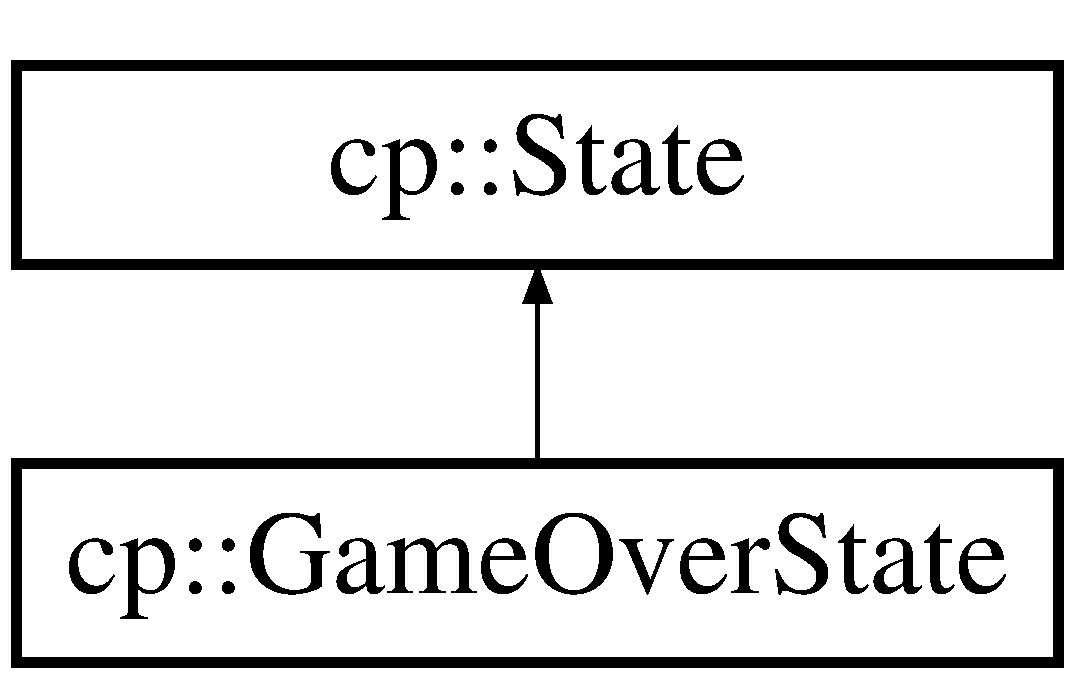
\includegraphics[height=2.000000cm]{classcp_1_1_game_over_state}
\end{center}
\end{figure}
\subsection*{Public Member Functions}
\begin{DoxyCompactItemize}
\item 
\mbox{\Hypertarget{classcp_1_1_game_over_state_a8899ce7260ab74b44864daa533115e2c}\label{classcp_1_1_game_over_state_a8899ce7260ab74b44864daa533115e2c}} 
{\bfseries Game\+Over\+State} (Game\+Data\+Ref \+\_\+data)
\item 
\mbox{\Hypertarget{classcp_1_1_game_over_state_a17c6bda552b241b54306dfe6845697be}\label{classcp_1_1_game_over_state_a17c6bda552b241b54306dfe6845697be}} 
void {\bfseries init} ()
\item 
\mbox{\Hypertarget{classcp_1_1_game_over_state_a24406ce1a3f8e697ff1444dc9f2427c9}\label{classcp_1_1_game_over_state_a24406ce1a3f8e697ff1444dc9f2427c9}} 
void {\bfseries handle\+\_\+input} (float delta)
\item 
\mbox{\Hypertarget{classcp_1_1_game_over_state_a63de2b959443ef1f208d1d1e69e389f1}\label{classcp_1_1_game_over_state_a63de2b959443ef1f208d1d1e69e389f1}} 
void {\bfseries draw} (float delta)
\item 
\mbox{\Hypertarget{classcp_1_1_game_over_state_af9154256a66528e017dfcff73289b2d6}\label{classcp_1_1_game_over_state_af9154256a66528e017dfcff73289b2d6}} 
void {\bfseries update} (float delta)
\end{DoxyCompactItemize}
\subsection*{Public Attributes}
\begin{DoxyCompactItemize}
\item 
\mbox{\Hypertarget{classcp_1_1_game_over_state_acdeb1263f0f41328538cd29d451df30e}\label{classcp_1_1_game_over_state_acdeb1263f0f41328538cd29d451df30e}} 
sf\+::\+Font {\bfseries font}
\item 
\mbox{\Hypertarget{classcp_1_1_game_over_state_ae6d660908d6e67f5f0bb94ff2b096682}\label{classcp_1_1_game_over_state_ae6d660908d6e67f5f0bb94ff2b096682}} 
sf\+::\+Text {\bfseries text}
\end{DoxyCompactItemize}


The documentation for this class was generated from the following files\+:\begin{DoxyCompactItemize}
\item 
include/\+States/Game\+Over\+State.\+hpp\item 
libs/Game\+Over\+State.\+cpp\end{DoxyCompactItemize}

\hypertarget{classcp_1_1_game_simulation_log}{}\section{cp\+:\+:Game\+Simulation\+Log Class Reference}
\label{classcp_1_1_game_simulation_log}\index{cp\+::\+Game\+Simulation\+Log@{cp\+::\+Game\+Simulation\+Log}}


The documentation for this class was generated from the following file\+:\begin{DoxyCompactItemize}
\item 
include/\+States/\hyperlink{_game_simulator_8hpp}{Game\+Simulator.\+hpp}\end{DoxyCompactItemize}

\hypertarget{classcp_1_1_game_simulator}{}\section{cp\+:\+:Game\+Simulator Class Reference}
\label{classcp_1_1_game_simulator}\index{cp\+::\+Game\+Simulator@{cp\+::\+Game\+Simulator}}
\subsection*{Public Types}
\begin{DoxyCompactItemize}
\item 
\mbox{\Hypertarget{classcp_1_1_game_simulator_ab5c123bfd5895d6a98fa97e1ecf496f3}\label{classcp_1_1_game_simulator_ab5c123bfd5895d6a98fa97e1ecf496f3}} 
using {\bfseries ID} = long long int
\item 
\mbox{\Hypertarget{classcp_1_1_game_simulator_a293ce7623321b8622c6ad31a26c3a5ef}\label{classcp_1_1_game_simulator_a293ce7623321b8622c6ad31a26c3a5ef}} 
using {\bfseries input\+\_\+type} = Bot\+::input\+\_\+type
\item 
\mbox{\Hypertarget{classcp_1_1_game_simulator_ac69abb25c0cc70fe1ae3c0b4454e382a}\label{classcp_1_1_game_simulator_ac69abb25c0cc70fe1ae3c0b4454e382a}} 
using {\bfseries input\+\_\+return\+\_\+type} = std\+::pair$<$ ID, input\+\_\+type $>$
\end{DoxyCompactItemize}
\subsection*{Public Member Functions}
\begin{DoxyCompactItemize}
\item 
\hyperlink{classcp_1_1_game_simulator_a5f1df55a988bcd5aa19dc37a3f2f64f8}{Game\+Simulator} (Game\+Data\+Ref res\+\_\+store)
\begin{DoxyCompactList}\small\item\em Construct a new \hyperlink{classcp_1_1_game}{Game} Simulator\+:\+: \hyperlink{classcp_1_1_game}{Game} Simulator object. \end{DoxyCompactList}\item 
\mbox{\Hypertarget{classcp_1_1_game_simulator_a64ab0578e27b01b32c492b3d48676a23}\label{classcp_1_1_game_simulator_a64ab0578e27b01b32c492b3d48676a23}} 
\hyperlink{classcp_1_1_game_simulator_a64ab0578e27b01b32c492b3d48676a23}{$\sim$\+Game\+Simulator} ()
\begin{DoxyCompactList}\small\item\em Destroy the \hyperlink{classcp_1_1_game}{Game} Simulator\+:\+: \hyperlink{classcp_1_1_game}{Game} Simulator object. \end{DoxyCompactList}\item 
\hyperlink{classcp_1_1_game_simulator_snap}{Game\+Simulator\+Snap} \hyperlink{classcp_1_1_game_simulator_a2997be5cd3e69cd47f12cf36739d1c86}{get\+\_\+current\+\_\+snap} (Snap\+Flag flag)
\begin{DoxyCompactList}\small\item\em Get the current snap object. \end{DoxyCompactList}\item 
\hyperlink{classcp_1_1_game_simulation_log}{Game\+Simulation\+Log} \hyperlink{classcp_1_1_game_simulator_af91c09a6455555fdcfd94278e0c85312}{use\+\_\+snap} (const \hyperlink{classcp_1_1_game_simulator_snap}{Game\+Simulator\+Snap} \&snap, bool is\+\_\+forced=true)
\begin{DoxyCompactList}\small\item\em Updates the game simulation with the snap provided. \end{DoxyCompactList}\item 
\mbox{\Hypertarget{classcp_1_1_game_simulator_aabb25f4078d8fe5a54cea4952da49aa7}\label{classcp_1_1_game_simulator_aabb25f4078d8fe5a54cea4952da49aa7}} 
float {\bfseries distance} (\hyperlink{classcp_1_1entity__info}{entity\+\_\+info} \&a, \hyperlink{classcp_1_1entity__info}{entity\+\_\+info} \&b)
\item 
\mbox{\Hypertarget{classcp_1_1_game_simulator_a5c67da11f83aef5976895104f24dd70a}\label{classcp_1_1_game_simulator_a5c67da11f83aef5976895104f24dd70a}} 
void {\bfseries output} (\hyperlink{classcp_1_1entity__info}{entity\+\_\+info} \&a, \hyperlink{classcp_1_1entity__info}{entity\+\_\+info} \&b, std\+::vector$<$ bool $>$ \&input)
\item 
\mbox{\Hypertarget{classcp_1_1_game_simulator_a69efe33b404b070b07cec35e8d396c34}\label{classcp_1_1_game_simulator_a69efe33b404b070b07cec35e8d396c34}} 
void {\bfseries A\+I\+\_\+bot\+\_\+output} ()
\item 
\mbox{\Hypertarget{classcp_1_1_game_simulator_a4840d30b48ce4493ae4631387b914bc8}\label{classcp_1_1_game_simulator_a4840d30b48ce4493ae4631387b914bc8}} 
void {\bfseries generate\+\_\+log} ()
\item 
\mbox{\Hypertarget{classcp_1_1_game_simulator_acc82bdb23b927ee977fa5fdea29f4bc1}\label{classcp_1_1_game_simulator_acc82bdb23b927ee977fa5fdea29f4bc1}} 
void \hyperlink{classcp_1_1_game_simulator_acc82bdb23b927ee977fa5fdea29f4bc1}{init} ()
\begin{DoxyCompactList}\small\item\em Initializing all the entities in the \hyperlink{classcp_1_1_game}{Game}. \end{DoxyCompactList}\item 
void \hyperlink{classcp_1_1_game_simulator_ab41fde16054aafe338df7e4d5590eeae}{handle\+\_\+input} (float delta)
\begin{DoxyCompactList}\small\item\em This function provide space for doing handle input on all the entities. \end{DoxyCompactList}\item 
void \hyperlink{classcp_1_1_game_simulator_a52971edf1b8258ea825d8c2fec9e30d1}{draw} (float delta)
\begin{DoxyCompactList}\small\item\em This method provide the room for drawing all the elements on the window. \end{DoxyCompactList}\item 
void \hyperlink{classcp_1_1_game_simulator_a6a0cd908ab20a8b776620f168846730c}{update} (float delta)
\begin{DoxyCompactList}\small\item\em This method provide room for updating all the entities. \end{DoxyCompactList}\item 
\hyperlink{classcp_1_1_player_car}{Player\+Car} \hyperlink{classcp_1_1_game_simulator_ae0a0e21217dfffba34e067ebc77c9031}{generate\+\_\+bot} (const \hyperlink{classcp_1_1entity__info}{entity\+\_\+info} \&info)
\begin{DoxyCompactList}\small\item\em Utility function to generate the bots. \end{DoxyCompactList}\item 
bool \hyperlink{classcp_1_1_game_simulator_addf94d6211247e0f2c77cae8541f09d8}{add\+\_\+external\+\_\+player} (ID id)
\begin{DoxyCompactList}\small\item\em Adds external player with their id. \end{DoxyCompactList}\item 
bool \hyperlink{classcp_1_1_game_simulator_ae06e0ba47d8d535f462c072daaae16e4}{add\+\_\+bot\+\_\+players} ()
\begin{DoxyCompactList}\small\item\em Adds a bot player in the simulation. \end{DoxyCompactList}\item 
void \hyperlink{classcp_1_1_game_simulator_a5f2d1089b8a260f62138d6f07ba404a7}{remove\+\_\+ext\+\_\+player} (ID id)
\begin{DoxyCompactList}\small\item\em Removes an external player if available. \end{DoxyCompactList}\item 
bool \hyperlink{classcp_1_1_game_simulator_a04e844bdf85698a60c978d173116e1e0}{update\+\_\+main\+\_\+player} (ID id)
\begin{DoxyCompactList}\small\item\em Update the main player of the simulation. \end{DoxyCompactList}\item 
bool \hyperlink{classcp_1_1_game_simulator_aafaedf9736a754a59b8a4c35db3fdac3}{is\+\_\+main\+\_\+player\+\_\+available} ()
\begin{DoxyCompactList}\small\item\em Checks if main player is in the simulation. \end{DoxyCompactList}\item 
\mbox{\Hypertarget{classcp_1_1_game_simulator_a54d498d40cb2d615039d8d03dfc76239}\label{classcp_1_1_game_simulator_a54d498d40cb2d615039d8d03dfc76239}} 
input\+\_\+return\+\_\+type {\bfseries get\+\_\+input} ()
\item 
\mbox{\Hypertarget{classcp_1_1_game_simulator_a31162ab043dad3357cb7f6cda7861618}\label{classcp_1_1_game_simulator_a31162ab043dad3357cb7f6cda7861618}} 
void {\bfseries focus\+\_\+on} (ID id)
\end{DoxyCompactItemize}
\subsection*{Public Attributes}
\begin{DoxyCompactItemize}
\item 
\mbox{\Hypertarget{classcp_1_1_game_simulator_a99927634c5bc41cdf6c690706bb5c848}\label{classcp_1_1_game_simulator_a99927634c5bc41cdf6c690706bb5c848}} 
std\+::ofstream {\bfseries fout}
\end{DoxyCompactItemize}


\subsection{Constructor \& Destructor Documentation}
\mbox{\Hypertarget{classcp_1_1_game_simulator_a5f1df55a988bcd5aa19dc37a3f2f64f8}\label{classcp_1_1_game_simulator_a5f1df55a988bcd5aa19dc37a3f2f64f8}} 
\index{cp\+::\+Game\+Simulator@{cp\+::\+Game\+Simulator}!Game\+Simulator@{Game\+Simulator}}
\index{Game\+Simulator@{Game\+Simulator}!cp\+::\+Game\+Simulator@{cp\+::\+Game\+Simulator}}
\subsubsection{\texorpdfstring{Game\+Simulator()}{GameSimulator()}}
{\footnotesize\ttfamily cp\+::\+Game\+Simulator\+::\+Game\+Simulator (\begin{DoxyParamCaption}\item[{Game\+Data\+Ref}]{res\+\_\+store }\end{DoxyParamCaption})}



Construct a new \hyperlink{classcp_1_1_game}{Game} Simulator\+:\+: \hyperlink{classcp_1_1_game}{Game} Simulator object. 


\begin{DoxyParams}{Parameters}
{\em res\+\_\+store} & Contains all resource managers \\
\hline
\end{DoxyParams}


\subsection{Member Function Documentation}
\mbox{\Hypertarget{classcp_1_1_game_simulator_ae06e0ba47d8d535f462c072daaae16e4}\label{classcp_1_1_game_simulator_ae06e0ba47d8d535f462c072daaae16e4}} 
\index{cp\+::\+Game\+Simulator@{cp\+::\+Game\+Simulator}!add\+\_\+bot\+\_\+players@{add\+\_\+bot\+\_\+players}}
\index{add\+\_\+bot\+\_\+players@{add\+\_\+bot\+\_\+players}!cp\+::\+Game\+Simulator@{cp\+::\+Game\+Simulator}}
\subsubsection{\texorpdfstring{add\+\_\+bot\+\_\+players()}{add\_bot\_players()}}
{\footnotesize\ttfamily bool cp\+::\+Game\+Simulator\+::add\+\_\+bot\+\_\+players (\begin{DoxyParamCaption}{ }\end{DoxyParamCaption})\hspace{0.3cm}{\ttfamily [inline]}}



Adds a bot player in the simulation. 

\begin{DoxyReturn}{Returns}
true Returns true if bot addition was a success. 

false Returns false otherwise. 
\end{DoxyReturn}
\mbox{\Hypertarget{classcp_1_1_game_simulator_addf94d6211247e0f2c77cae8541f09d8}\label{classcp_1_1_game_simulator_addf94d6211247e0f2c77cae8541f09d8}} 
\index{cp\+::\+Game\+Simulator@{cp\+::\+Game\+Simulator}!add\+\_\+external\+\_\+player@{add\+\_\+external\+\_\+player}}
\index{add\+\_\+external\+\_\+player@{add\+\_\+external\+\_\+player}!cp\+::\+Game\+Simulator@{cp\+::\+Game\+Simulator}}
\subsubsection{\texorpdfstring{add\+\_\+external\+\_\+player()}{add\_external\_player()}}
{\footnotesize\ttfamily bool cp\+::\+Game\+Simulator\+::add\+\_\+external\+\_\+player (\begin{DoxyParamCaption}\item[{ID}]{id }\end{DoxyParamCaption})\hspace{0.3cm}{\ttfamily [inline]}}



Adds external player with their id. 


\begin{DoxyParams}{Parameters}
{\em id} & This is the id they have requested. \\
\hline
\end{DoxyParams}
\begin{DoxyReturn}{Returns}
true if player addition is successful 

false if player addition fails 
\end{DoxyReturn}
\mbox{\Hypertarget{classcp_1_1_game_simulator_a52971edf1b8258ea825d8c2fec9e30d1}\label{classcp_1_1_game_simulator_a52971edf1b8258ea825d8c2fec9e30d1}} 
\index{cp\+::\+Game\+Simulator@{cp\+::\+Game\+Simulator}!draw@{draw}}
\index{draw@{draw}!cp\+::\+Game\+Simulator@{cp\+::\+Game\+Simulator}}
\subsubsection{\texorpdfstring{draw()}{draw()}}
{\footnotesize\ttfamily void cp\+::\+Game\+Simulator\+::draw (\begin{DoxyParamCaption}\item[{float}]{delta }\end{DoxyParamCaption})}



This method provide the room for drawing all the elements on the window. 


\begin{DoxyParams}{Parameters}
{\em delta} & Time difference between two accumulator \\
\hline
\end{DoxyParams}
\mbox{\Hypertarget{classcp_1_1_game_simulator_ae0a0e21217dfffba34e067ebc77c9031}\label{classcp_1_1_game_simulator_ae0a0e21217dfffba34e067ebc77c9031}} 
\index{cp\+::\+Game\+Simulator@{cp\+::\+Game\+Simulator}!generate\+\_\+bot@{generate\+\_\+bot}}
\index{generate\+\_\+bot@{generate\+\_\+bot}!cp\+::\+Game\+Simulator@{cp\+::\+Game\+Simulator}}
\subsubsection{\texorpdfstring{generate\+\_\+bot()}{generate\_bot()}}
{\footnotesize\ttfamily \hyperlink{classcp_1_1_player_car}{Player\+Car} cp\+::\+Game\+Simulator\+::generate\+\_\+bot (\begin{DoxyParamCaption}\item[{const \hyperlink{classcp_1_1entity__info}{entity\+\_\+info} \&}]{info }\end{DoxyParamCaption})}



Utility function to generate the bots. 


\begin{DoxyParams}{Parameters}
{\em info} & uses the info provided in the argument to generate the bot \\
\hline
\end{DoxyParams}
\begin{DoxyReturn}{Returns}
\hyperlink{classcp_1_1_player_car}{Player\+Car} Returns the generated object 
\end{DoxyReturn}
\mbox{\Hypertarget{classcp_1_1_game_simulator_a2997be5cd3e69cd47f12cf36739d1c86}\label{classcp_1_1_game_simulator_a2997be5cd3e69cd47f12cf36739d1c86}} 
\index{cp\+::\+Game\+Simulator@{cp\+::\+Game\+Simulator}!get\+\_\+current\+\_\+snap@{get\+\_\+current\+\_\+snap}}
\index{get\+\_\+current\+\_\+snap@{get\+\_\+current\+\_\+snap}!cp\+::\+Game\+Simulator@{cp\+::\+Game\+Simulator}}
\subsubsection{\texorpdfstring{get\+\_\+current\+\_\+snap()}{get\_current\_snap()}}
{\footnotesize\ttfamily \hyperlink{classcp_1_1_game_simulator_snap}{Game\+Simulator\+Snap} cp\+::\+Game\+Simulator\+::get\+\_\+current\+\_\+snap (\begin{DoxyParamCaption}\item[{Snap\+Flag}]{flag }\end{DoxyParamCaption})}



Get the current snap object. 

Returns a snap of the game such that the simulation can be recreated.


\begin{DoxyParams}{Parameters}
{\em flag} & \\
\hline
\end{DoxyParams}
\begin{DoxyReturn}{Returns}
\hyperlink{classcp_1_1_game_simulator_snap}{Game\+Simulator\+Snap}
\end{DoxyReturn}

\begin{DoxyParams}{Parameters}
{\em flag} & Type of snap that you want (N\+E\+T\+W\+O\+R\+K/\+O\+F\+F\+L\+I\+NE) \\
\hline
\end{DoxyParams}
\begin{DoxyReturn}{Returns}
\hyperlink{classcp_1_1_game_simulator_snap}{Game\+Simulator\+Snap} The current snap of the game. 
\end{DoxyReturn}
\mbox{\Hypertarget{classcp_1_1_game_simulator_ab41fde16054aafe338df7e4d5590eeae}\label{classcp_1_1_game_simulator_ab41fde16054aafe338df7e4d5590eeae}} 
\index{cp\+::\+Game\+Simulator@{cp\+::\+Game\+Simulator}!handle\+\_\+input@{handle\+\_\+input}}
\index{handle\+\_\+input@{handle\+\_\+input}!cp\+::\+Game\+Simulator@{cp\+::\+Game\+Simulator}}
\subsubsection{\texorpdfstring{handle\+\_\+input()}{handle\_input()}}
{\footnotesize\ttfamily void cp\+::\+Game\+Simulator\+::handle\+\_\+input (\begin{DoxyParamCaption}\item[{float}]{delta }\end{DoxyParamCaption})}



This function provide space for doing handle input on all the entities. 


\begin{DoxyParams}{Parameters}
{\em delta} & The time difference between two frames \\
\hline
\end{DoxyParams}
\mbox{\Hypertarget{classcp_1_1_game_simulator_aafaedf9736a754a59b8a4c35db3fdac3}\label{classcp_1_1_game_simulator_aafaedf9736a754a59b8a4c35db3fdac3}} 
\index{cp\+::\+Game\+Simulator@{cp\+::\+Game\+Simulator}!is\+\_\+main\+\_\+player\+\_\+available@{is\+\_\+main\+\_\+player\+\_\+available}}
\index{is\+\_\+main\+\_\+player\+\_\+available@{is\+\_\+main\+\_\+player\+\_\+available}!cp\+::\+Game\+Simulator@{cp\+::\+Game\+Simulator}}
\subsubsection{\texorpdfstring{is\+\_\+main\+\_\+player\+\_\+available()}{is\_main\_player\_available()}}
{\footnotesize\ttfamily bool cp\+::\+Game\+Simulator\+::is\+\_\+main\+\_\+player\+\_\+available (\begin{DoxyParamCaption}{ }\end{DoxyParamCaption})\hspace{0.3cm}{\ttfamily [inline]}}



Checks if main player is in the simulation. 

\begin{DoxyReturn}{Returns}
true if main player is found. 

false if main player not found. 
\end{DoxyReturn}
\mbox{\Hypertarget{classcp_1_1_game_simulator_a5f2d1089b8a260f62138d6f07ba404a7}\label{classcp_1_1_game_simulator_a5f2d1089b8a260f62138d6f07ba404a7}} 
\index{cp\+::\+Game\+Simulator@{cp\+::\+Game\+Simulator}!remove\+\_\+ext\+\_\+player@{remove\+\_\+ext\+\_\+player}}
\index{remove\+\_\+ext\+\_\+player@{remove\+\_\+ext\+\_\+player}!cp\+::\+Game\+Simulator@{cp\+::\+Game\+Simulator}}
\subsubsection{\texorpdfstring{remove\+\_\+ext\+\_\+player()}{remove\_ext\_player()}}
{\footnotesize\ttfamily void cp\+::\+Game\+Simulator\+::remove\+\_\+ext\+\_\+player (\begin{DoxyParamCaption}\item[{ID}]{id }\end{DoxyParamCaption})\hspace{0.3cm}{\ttfamily [inline]}}



Removes an external player if available. 


\begin{DoxyParams}{Parameters}
{\em id} & Id of the external player to remove. \\
\hline
\end{DoxyParams}
\mbox{\Hypertarget{classcp_1_1_game_simulator_a6a0cd908ab20a8b776620f168846730c}\label{classcp_1_1_game_simulator_a6a0cd908ab20a8b776620f168846730c}} 
\index{cp\+::\+Game\+Simulator@{cp\+::\+Game\+Simulator}!update@{update}}
\index{update@{update}!cp\+::\+Game\+Simulator@{cp\+::\+Game\+Simulator}}
\subsubsection{\texorpdfstring{update()}{update()}}
{\footnotesize\ttfamily void cp\+::\+Game\+Simulator\+::update (\begin{DoxyParamCaption}\item[{float}]{delta }\end{DoxyParamCaption})}



This method provide room for updating all the entities. 


\begin{DoxyParams}{Parameters}
{\em delta} & This is the time difference between two frames. \\
\hline
\end{DoxyParams}
\mbox{\Hypertarget{classcp_1_1_game_simulator_a04e844bdf85698a60c978d173116e1e0}\label{classcp_1_1_game_simulator_a04e844bdf85698a60c978d173116e1e0}} 
\index{cp\+::\+Game\+Simulator@{cp\+::\+Game\+Simulator}!update\+\_\+main\+\_\+player@{update\+\_\+main\+\_\+player}}
\index{update\+\_\+main\+\_\+player@{update\+\_\+main\+\_\+player}!cp\+::\+Game\+Simulator@{cp\+::\+Game\+Simulator}}
\subsubsection{\texorpdfstring{update\+\_\+main\+\_\+player()}{update\_main\_player()}}
{\footnotesize\ttfamily bool cp\+::\+Game\+Simulator\+::update\+\_\+main\+\_\+player (\begin{DoxyParamCaption}\item[{ID}]{id }\end{DoxyParamCaption})\hspace{0.3cm}{\ttfamily [inline]}}



Update the main player of the simulation. 


\begin{DoxyParams}{Parameters}
{\em id} & Update the main player with ID \\
\hline
\end{DoxyParams}
\begin{DoxyReturn}{Returns}
true If operation is succesfull. 

false If operation is unsuccessfull. 
\end{DoxyReturn}
\mbox{\Hypertarget{classcp_1_1_game_simulator_af91c09a6455555fdcfd94278e0c85312}\label{classcp_1_1_game_simulator_af91c09a6455555fdcfd94278e0c85312}} 
\index{cp\+::\+Game\+Simulator@{cp\+::\+Game\+Simulator}!use\+\_\+snap@{use\+\_\+snap}}
\index{use\+\_\+snap@{use\+\_\+snap}!cp\+::\+Game\+Simulator@{cp\+::\+Game\+Simulator}}
\subsubsection{\texorpdfstring{use\+\_\+snap()}{use\_snap()}}
{\footnotesize\ttfamily \hyperlink{classcp_1_1_game_simulation_log}{Game\+Simulation\+Log} cp\+::\+Game\+Simulator\+::use\+\_\+snap (\begin{DoxyParamCaption}\item[{const \hyperlink{classcp_1_1_game_simulator_snap}{Game\+Simulator\+Snap} \&}]{snap,  }\item[{bool}]{is\+\_\+forced = {\ttfamily true} }\end{DoxyParamCaption})}



Updates the game simulation with the snap provided. 

Calling this function will replace all the entities and their info with info in snap argument.


\begin{DoxyParams}{Parameters}
{\em snap} & Refers to the snap of the game to update the simulation with. \\
\hline
{\em is\+\_\+forced} & If set then forcefully overwrites the snap provided. \\
\hline
\end{DoxyParams}
\begin{DoxyReturn}{Returns}
\hyperlink{classcp_1_1_game_simulation_log}{Game\+Simulation\+Log} Returns a log describing whether the replacment was partial/discarded/sucess.
\end{DoxyReturn}

\begin{DoxyParams}{Parameters}
{\em snap} & Snap that you want to replace the Game\+Info with \\
\hline
{\em is\+\_\+forced} & Forcefully replace all the info with the snap info \\
\hline
\end{DoxyParams}
\begin{DoxyReturn}{Returns}
\hyperlink{classcp_1_1_game_simulation_log}{Game\+Simulation\+Log} Returns a log file illustrating the success of the operation. 
\end{DoxyReturn}


The documentation for this class was generated from the following files\+:\begin{DoxyCompactItemize}
\item 
include/\+States/\hyperlink{_game_simulator_8hpp}{Game\+Simulator.\+hpp}\item 
libs/\hyperlink{_game_simulator_8cpp}{Game\+Simulator.\+cpp}\end{DoxyCompactItemize}

\hypertarget{classcp_1_1_game_simulator_snap}{}\section{cp\+:\+:Game\+Simulator\+Snap Class Reference}
\label{classcp_1_1_game_simulator_snap}\index{cp\+::\+Game\+Simulator\+Snap@{cp\+::\+Game\+Simulator\+Snap}}
\subsection*{Public Member Functions}
\begin{DoxyCompactItemize}
\item 
\mbox{\Hypertarget{classcp_1_1_game_simulator_snap_ab9923e29a6ffd927c5f286210eb4d2c4}\label{classcp_1_1_game_simulator_snap_ab9923e29a6ffd927c5f286210eb4d2c4}} 
{\bfseries Game\+Simulator\+Snap} (int a, int b, int c, int d, std\+::map$<$ ID, \hyperlink{classcp_1_1_player_car}{Player\+Car} $>$ \&players\+\_\+map)
\end{DoxyCompactItemize}
\subsection*{Friends}
\begin{DoxyCompactItemize}
\item 
\mbox{\Hypertarget{classcp_1_1_game_simulator_snap_a5914b299fccea3f3c5ae2224cd4e2b3e}\label{classcp_1_1_game_simulator_snap_a5914b299fccea3f3c5ae2224cd4e2b3e}} 
class {\bfseries Game\+Simulator}
\item 
\mbox{\Hypertarget{classcp_1_1_game_simulator_snap_a1f116c2d145732cc04ee5dc75555fe75}\label{classcp_1_1_game_simulator_snap_a1f116c2d145732cc04ee5dc75555fe75}} 
std\+::ofstream \& {\bfseries operator$<$$<$} (std\+::ofstream \&fout, const \hyperlink{classcp_1_1_game_simulator_snap}{Game\+Simulator\+Snap} \&snap)
\item 
\mbox{\Hypertarget{classcp_1_1_game_simulator_snap_a8153e2b1eb4cfc4652145b5adcd2b402}\label{classcp_1_1_game_simulator_snap_a8153e2b1eb4cfc4652145b5adcd2b402}} 
sf\+::\+Packet \& {\bfseries operator$<$$<$} (sf\+::\+Packet \&fout, const \hyperlink{classcp_1_1_game_simulator_snap}{Game\+Simulator\+Snap} \&snap)
\item 
\mbox{\Hypertarget{classcp_1_1_game_simulator_snap_ad7c6e04d3ba040f6bef4f5d6a095989d}\label{classcp_1_1_game_simulator_snap_ad7c6e04d3ba040f6bef4f5d6a095989d}} 
sf\+::\+Packet \& {\bfseries operator$>$$>$} (sf\+::\+Packet \&fin, \hyperlink{classcp_1_1_game_simulator_snap}{Game\+Simulator\+Snap} \&snap)
\end{DoxyCompactItemize}


The documentation for this class was generated from the following file\+:\begin{DoxyCompactItemize}
\item 
include/\+States/\hyperlink{_game_simulator_8hpp}{Game\+Simulator.\+hpp}\end{DoxyCompactItemize}

\hypertarget{classcp_1_1_game_state}{}\section{cp\+:\+:Game\+State Class Reference}
\label{classcp_1_1_game_state}\index{cp\+::\+Game\+State@{cp\+::\+Game\+State}}
Inheritance diagram for cp\+:\+:Game\+State\+:\begin{figure}[H]
\begin{center}
\leavevmode
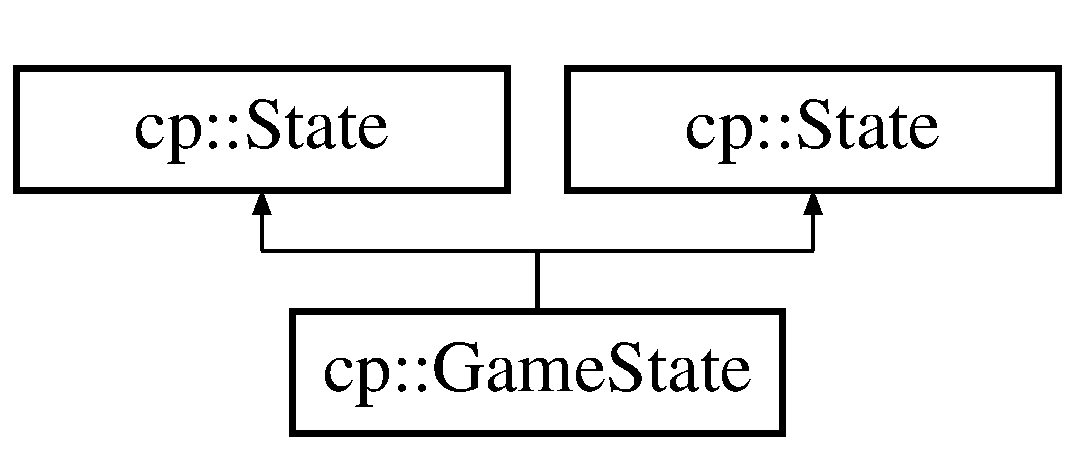
\includegraphics[height=2.000000cm]{classcp_1_1_game_state}
\end{center}
\end{figure}
\subsection*{Public Types}
\begin{DoxyCompactItemize}
\item 
\mbox{\Hypertarget{classcp_1_1_game_state_ae6b57da0779db6b2c6458aa484496d61}\label{classcp_1_1_game_state_ae6b57da0779db6b2c6458aa484496d61}} 
typedef std\+::shared\+\_\+ptr$<$ \hyperlink{classcp_1_1_player_car}{Player\+Car} $>$ {\bfseries Car\+Ref}
\end{DoxyCompactItemize}
\subsection*{Public Member Functions}
\begin{DoxyCompactItemize}
\item 
\mbox{\Hypertarget{classcp_1_1_game_state_af8b15ea02a00d2952500404ba4ae63b8}\label{classcp_1_1_game_state_af8b15ea02a00d2952500404ba4ae63b8}} 
{\bfseries Game\+State} (Game\+Data\+Ref \+\_\+data)
\item 
\mbox{\Hypertarget{classcp_1_1_game_state_a91fc8fff6e06a8fddb4b4ea785bdcf0e}\label{classcp_1_1_game_state_a91fc8fff6e06a8fddb4b4ea785bdcf0e}} 
void {\bfseries init} ()
\item 
\mbox{\Hypertarget{classcp_1_1_game_state_af9c8395fedd3343337f2e249669d8e52}\label{classcp_1_1_game_state_af9c8395fedd3343337f2e249669d8e52}} 
void {\bfseries handle\+\_\+input} (float delta)
\item 
\mbox{\Hypertarget{classcp_1_1_game_state_a17b81f0c87209d967c571393b3a493d9}\label{classcp_1_1_game_state_a17b81f0c87209d967c571393b3a493d9}} 
void {\bfseries draw} (float delta)
\item 
\mbox{\Hypertarget{classcp_1_1_game_state_abe654ab4d56344d7897b5e93be36e5f3}\label{classcp_1_1_game_state_abe654ab4d56344d7897b5e93be36e5f3}} 
void {\bfseries update} (float delta)
\item 
\mbox{\Hypertarget{classcp_1_1_game_state_a34e5851e826d9b73c80648d86ca729de}\label{classcp_1_1_game_state_a34e5851e826d9b73c80648d86ca729de}} 
void {\bfseries draw\+Sprite} (\hyperlink{classcp_1_1_line}{Line} \&line)
\item 
\mbox{\Hypertarget{classcp_1_1_game_state_af8b15ea02a00d2952500404ba4ae63b8}\label{classcp_1_1_game_state_af8b15ea02a00d2952500404ba4ae63b8}} 
{\bfseries Game\+State} (Game\+Data\+Ref \+\_\+data)
\item 
\mbox{\Hypertarget{classcp_1_1_game_state_aaaa06069d85774c0dca85a99989da467}\label{classcp_1_1_game_state_aaaa06069d85774c0dca85a99989da467}} 
virtual void {\bfseries init} ()
\item 
\mbox{\Hypertarget{classcp_1_1_game_state_a326eebfad824224c4d01588839c42e3d}\label{classcp_1_1_game_state_a326eebfad824224c4d01588839c42e3d}} 
virtual void {\bfseries handle\+\_\+input} (float delta)
\end{DoxyCompactItemize}
\subsection*{Static Public Member Functions}
\begin{DoxyCompactItemize}
\item 
\mbox{\Hypertarget{classcp_1_1_game_state_aabbafbae2e0067041117d8395b246526}\label{classcp_1_1_game_state_aabbafbae2e0067041117d8395b246526}} 
static void {\bfseries network\+\_\+handler} (Game\+Data\+Ref data, std\+::shared\+\_\+ptr$<$ \hyperlink{classcp_1_1_player_car}{Player\+Car} $>$ car, std\+::shared\+\_\+ptr$<$ \hyperlink{classcp_1_1_bot}{Bot} $>$ bot)
\end{DoxyCompactItemize}


The documentation for this class was generated from the following files\+:\begin{DoxyCompactItemize}
\item 
include/Game\+State.\+hpp\item 
libs/Game\+State.\+cpp\end{DoxyCompactItemize}

\hypertarget{classcp_1_1_input_manager}{}\section{cp\+:\+:Input\+Manager Class Reference}
\label{classcp_1_1_input_manager}\index{cp\+::\+Input\+Manager@{cp\+::\+Input\+Manager}}
\subsection*{Public Member Functions}
\begin{DoxyCompactItemize}
\item 
\mbox{\Hypertarget{classcp_1_1_input_manager_add39dcc53f2dd57e84a698fb79bcc52d}\label{classcp_1_1_input_manager_add39dcc53f2dd57e84a698fb79bcc52d}} 
bool {\bfseries is\+\_\+sprite\+\_\+clicked} (sf\+::\+Sprite sprite, sf\+::\+Mouse\+::\+Button button, sf\+::\+Render\+Window \&window)
\item 
\mbox{\Hypertarget{classcp_1_1_input_manager_a2b44b7f5ba80f2c09021f939454c2e8d}\label{classcp_1_1_input_manager_a2b44b7f5ba80f2c09021f939454c2e8d}} 
sf\+::\+Vector2i {\bfseries get\+\_\+mouse\+\_\+position} (sf\+::\+Render\+Window \&window)
\item 
\mbox{\Hypertarget{classcp_1_1_input_manager_a2a3a288ebce452b2fbe2284c679ee815}\label{classcp_1_1_input_manager_a2a3a288ebce452b2fbe2284c679ee815}} 
void {\bfseries register\+\_\+input} (register\+\_\+input\+\_\+type input\+\_\+pair)
\item 
\mbox{\Hypertarget{classcp_1_1_input_manager_a25d2dbeef1b4444ea328ff9df945c983}\label{classcp_1_1_input_manager_a25d2dbeef1b4444ea328ff9df945c983}} 
input\+\_\+type {\bfseries get\+\_\+mask} (ID id)
\end{DoxyCompactItemize}


The documentation for this class was generated from the following files\+:\begin{DoxyCompactItemize}
\item 
include/\+Resource\+Managers/Input\+Manager.\+hpp\item 
libs/Input\+Manager.\+cpp\end{DoxyCompactItemize}

\hypertarget{classcp_1_1_line}{}\section{cp\+:\+:Line Class Reference}
\label{classcp_1_1_line}\index{cp\+::\+Line@{cp\+::\+Line}}
\subsection*{Public Attributes}
\begin{DoxyCompactItemize}
\item 
\mbox{\Hypertarget{classcp_1_1_line_ad39096f1a4e28c48faabce5a35f37be2}\label{classcp_1_1_line_ad39096f1a4e28c48faabce5a35f37be2}} 
float {\bfseries x} = 0
\item 
\mbox{\Hypertarget{classcp_1_1_line_afad3adaec719dfc12cc3e21215f8ece7}\label{classcp_1_1_line_afad3adaec719dfc12cc3e21215f8ece7}} 
float {\bfseries y} = 0
\item 
\mbox{\Hypertarget{classcp_1_1_line_aba081d41ceec386aed5f57a11cf90248}\label{classcp_1_1_line_aba081d41ceec386aed5f57a11cf90248}} 
float {\bfseries z} = 0
\item 
\mbox{\Hypertarget{classcp_1_1_line_aa9d0f92906b4d96fd91998ee51c42dd6}\label{classcp_1_1_line_aa9d0f92906b4d96fd91998ee51c42dd6}} 
float {\bfseries no\+\_\+curve\+\_\+Y} =0
\item 
\mbox{\Hypertarget{classcp_1_1_line_a8f4c6f1af7be861968c978a9f9afef52}\label{classcp_1_1_line_a8f4c6f1af7be861968c978a9f9afef52}} 
float {\bfseries no\+\_\+curve\+\_\+X} =0
\item 
\mbox{\Hypertarget{classcp_1_1_line_af47b43ff016a7bf5d86e353c3f6c4d45}\label{classcp_1_1_line_af47b43ff016a7bf5d86e353c3f6c4d45}} 
float {\bfseries X} = 0
\item 
\mbox{\Hypertarget{classcp_1_1_line_a60c932563c7ddfd43e715bdb61f31a4f}\label{classcp_1_1_line_a60c932563c7ddfd43e715bdb61f31a4f}} 
float {\bfseries Y} = 0
\item 
\mbox{\Hypertarget{classcp_1_1_line_a07318dd5254a404e229abab62e71570a}\label{classcp_1_1_line_a07318dd5254a404e229abab62e71570a}} 
float {\bfseries W} = 0
\item 
\mbox{\Hypertarget{classcp_1_1_line_ae9394f9580f35c70fba57db645c5ad8e}\label{classcp_1_1_line_ae9394f9580f35c70fba57db645c5ad8e}} 
float {\bfseries curve} = 0
\item 
\mbox{\Hypertarget{classcp_1_1_line_a32a7dc49aa15151b936e60f30cbe510e}\label{classcp_1_1_line_a32a7dc49aa15151b936e60f30cbe510e}} 
float {\bfseries spriteX} = 0
\item 
\mbox{\Hypertarget{classcp_1_1_line_a1415d74381e2468699200edde9e079d8}\label{classcp_1_1_line_a1415d74381e2468699200edde9e079d8}} 
float {\bfseries clip} = 0
\item 
\mbox{\Hypertarget{classcp_1_1_line_a56dde9092a2b1de12b8209475abaf416}\label{classcp_1_1_line_a56dde9092a2b1de12b8209475abaf416}} 
float {\bfseries scale} = 0
\item 
\mbox{\Hypertarget{classcp_1_1_line_af89dbcf4998239674db789519e50b48b}\label{classcp_1_1_line_af89dbcf4998239674db789519e50b48b}} 
sf\+::\+Sprite {\bfseries sprite}
\end{DoxyCompactItemize}


The documentation for this class was generated from the following file\+:\begin{DoxyCompactItemize}
\item 
include/\+Objects/Line.\+hpp\end{DoxyCompactItemize}

\hypertarget{classcp_1_1_main_menu_state}{}\section{cp\+:\+:Main\+Menu\+State Class Reference}
\label{classcp_1_1_main_menu_state}\index{cp\+::\+Main\+Menu\+State@{cp\+::\+Main\+Menu\+State}}
Inheritance diagram for cp\+:\+:Main\+Menu\+State\+:\begin{figure}[H]
\begin{center}
\leavevmode
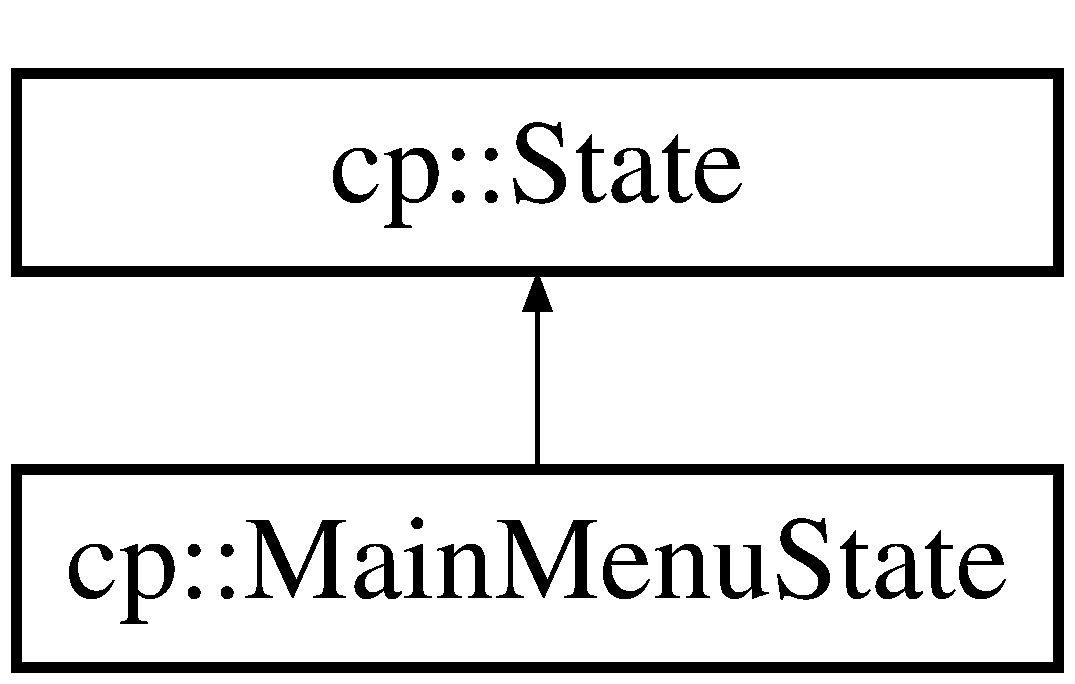
\includegraphics[height=2.000000cm]{classcp_1_1_main_menu_state}
\end{center}
\end{figure}
\subsection*{Public Member Functions}
\begin{DoxyCompactItemize}
\item 
\hyperlink{classcp_1_1_main_menu_state_a6ad449e3f50223aecb2e6639105235e2}{Main\+Menu\+State} (Game\+Data\+Ref \+\_\+data)
\begin{DoxyCompactList}\small\item\em Construct a new Main Menu \hyperlink{classcp_1_1_state}{State}\+:\+: Main Menu \hyperlink{classcp_1_1_state}{State} object. \end{DoxyCompactList}\item 
\mbox{\Hypertarget{classcp_1_1_main_menu_state_a3131fe5e7e02165b10e7dd04a67c7efd}\label{classcp_1_1_main_menu_state_a3131fe5e7e02165b10e7dd04a67c7efd}} 
void \hyperlink{classcp_1_1_main_menu_state_a3131fe5e7e02165b10e7dd04a67c7efd}{init} ()
\begin{DoxyCompactList}\small\item\em This function initializes all the components of Main\+Menu state. \end{DoxyCompactList}\item 
void \hyperlink{classcp_1_1_main_menu_state_a93e8ff7b27011d2f0bd0ad9a1da783e7}{handle\+\_\+input} (float delta)
\begin{DoxyCompactList}\small\item\em Provide interface to handle inputs in the Main\+Menu \hyperlink{classcp_1_1_state}{State}. \end{DoxyCompactList}\item 
void \hyperlink{classcp_1_1_main_menu_state_a1aabf2a9efa15f4cfbe6e6680472f955}{draw} (float delta)
\begin{DoxyCompactList}\small\item\em Function to draw all the components of Main\+Menu state on the screen. \end{DoxyCompactList}\item 
\mbox{\Hypertarget{classcp_1_1_main_menu_state_adf44b3ace26aa70890dfddc95221ba3e}\label{classcp_1_1_main_menu_state_adf44b3ace26aa70890dfddc95221ba3e}} 
void {\bfseries update} (float delta)
\end{DoxyCompactItemize}
\subsection*{Public Attributes}
\begin{DoxyCompactItemize}
\item 
\mbox{\Hypertarget{classcp_1_1_main_menu_state_a098358b03eb94f50879bacb68c18ae87}\label{classcp_1_1_main_menu_state_a098358b03eb94f50879bacb68c18ae87}} 
bool {\bfseries update\+\_\+required} = true
\end{DoxyCompactItemize}


\subsection{Constructor \& Destructor Documentation}
\mbox{\Hypertarget{classcp_1_1_main_menu_state_a6ad449e3f50223aecb2e6639105235e2}\label{classcp_1_1_main_menu_state_a6ad449e3f50223aecb2e6639105235e2}} 
\index{cp\+::\+Main\+Menu\+State@{cp\+::\+Main\+Menu\+State}!Main\+Menu\+State@{Main\+Menu\+State}}
\index{Main\+Menu\+State@{Main\+Menu\+State}!cp\+::\+Main\+Menu\+State@{cp\+::\+Main\+Menu\+State}}
\subsubsection{\texorpdfstring{Main\+Menu\+State()}{MainMenuState()}}
{\footnotesize\ttfamily cp\+::\+Main\+Menu\+State\+::\+Main\+Menu\+State (\begin{DoxyParamCaption}\item[{Game\+Data\+Ref}]{\+\_\+data }\end{DoxyParamCaption})}



Construct a new Main Menu \hyperlink{classcp_1_1_state}{State}\+:\+: Main Menu \hyperlink{classcp_1_1_state}{State} object. 


\begin{DoxyParams}{Parameters}
{\em \+\_\+data} & Pointer to all the resource managers and window \\
\hline
\end{DoxyParams}


\subsection{Member Function Documentation}
\mbox{\Hypertarget{classcp_1_1_main_menu_state_a1aabf2a9efa15f4cfbe6e6680472f955}\label{classcp_1_1_main_menu_state_a1aabf2a9efa15f4cfbe6e6680472f955}} 
\index{cp\+::\+Main\+Menu\+State@{cp\+::\+Main\+Menu\+State}!draw@{draw}}
\index{draw@{draw}!cp\+::\+Main\+Menu\+State@{cp\+::\+Main\+Menu\+State}}
\subsubsection{\texorpdfstring{draw()}{draw()}}
{\footnotesize\ttfamily void cp\+::\+Main\+Menu\+State\+::draw (\begin{DoxyParamCaption}\item[{float}]{delta }\end{DoxyParamCaption})\hspace{0.3cm}{\ttfamily [virtual]}}



Function to draw all the components of Main\+Menu state on the screen. 


\begin{DoxyParams}{Parameters}
{\em delta} & \\
\hline
\end{DoxyParams}


Implements \hyperlink{classcp_1_1_state}{cp\+::\+State}.

\mbox{\Hypertarget{classcp_1_1_main_menu_state_a93e8ff7b27011d2f0bd0ad9a1da783e7}\label{classcp_1_1_main_menu_state_a93e8ff7b27011d2f0bd0ad9a1da783e7}} 
\index{cp\+::\+Main\+Menu\+State@{cp\+::\+Main\+Menu\+State}!handle\+\_\+input@{handle\+\_\+input}}
\index{handle\+\_\+input@{handle\+\_\+input}!cp\+::\+Main\+Menu\+State@{cp\+::\+Main\+Menu\+State}}
\subsubsection{\texorpdfstring{handle\+\_\+input()}{handle\_input()}}
{\footnotesize\ttfamily void cp\+::\+Main\+Menu\+State\+::handle\+\_\+input (\begin{DoxyParamCaption}\item[{float}]{delta }\end{DoxyParamCaption})\hspace{0.3cm}{\ttfamily [virtual]}}



Provide interface to handle inputs in the Main\+Menu \hyperlink{classcp_1_1_state}{State}. 


\begin{DoxyParams}{Parameters}
{\em delta} & Time difference between two handle\+\_\+input call \\
\hline
\end{DoxyParams}


Implements \hyperlink{classcp_1_1_state}{cp\+::\+State}.



The documentation for this class was generated from the following files\+:\begin{DoxyCompactItemize}
\item 
include/\+States/Main\+Menu\+State.\+hpp\item 
libs/\hyperlink{_main_menu_state_8cpp}{Main\+Menu\+State.\+cpp}\end{DoxyCompactItemize}

\hypertarget{classcp_1_1_network_manager}{}\section{cp\+:\+:Network\+Manager Class Reference}
\label{classcp_1_1_network_manager}\index{cp\+::\+Network\+Manager@{cp\+::\+Network\+Manager}}
\subsection*{Static Public Member Functions}
\begin{DoxyCompactItemize}
\item 
\mbox{\Hypertarget{classcp_1_1_network_manager_ab8f3c5d78ac3b03baba90b912c5fe8d6}\label{classcp_1_1_network_manager_ab8f3c5d78ac3b03baba90b912c5fe8d6}} 
static void {\bfseries create\+Server} ()
\item 
\mbox{\Hypertarget{classcp_1_1_network_manager_aa0eb43e50d562372c9d4d14a96b76346}\label{classcp_1_1_network_manager_aa0eb43e50d562372c9d4d14a96b76346}} 
static void {\bfseries create\+Client} ()
\item 
\mbox{\Hypertarget{classcp_1_1_network_manager_aec8af90063036824008ffd0390a59844}\label{classcp_1_1_network_manager_aec8af90063036824008ffd0390a59844}} 
static void {\bfseries run} (int type)
\item 
\mbox{\Hypertarget{classcp_1_1_network_manager_a207bc3b12643d96cd779b3c084c5a2cc}\label{classcp_1_1_network_manager_a207bc3b12643d96cd779b3c084c5a2cc}} 
static void {\bfseries send\+Data} (sf\+::\+Vector3f pos)
\item 
\mbox{\Hypertarget{classcp_1_1_network_manager_af92420957986df43d458355b3e0ecd0a}\label{classcp_1_1_network_manager_af92420957986df43d458355b3e0ecd0a}} 
static void {\bfseries send} (sf\+::\+Vector3f pos)
\end{DoxyCompactItemize}
\subsection*{Public Attributes}
\begin{DoxyCompactItemize}
\item 
\mbox{\Hypertarget{classcp_1_1_network_manager_a31a23545e4ed63151981fcfdd464f0ed}\label{classcp_1_1_network_manager_a31a23545e4ed63151981fcfdd464f0ed}} 
sf\+::\+Socket\+::\+Status {\bfseries s\+\_\+status}
\item 
\mbox{\Hypertarget{classcp_1_1_network_manager_ad234304dd0a7921c4911c845ebddbe15}\label{classcp_1_1_network_manager_ad234304dd0a7921c4911c845ebddbe15}} 
sf\+::\+Socket\+::\+Status {\bfseries c\+\_\+status}
\item 
\mbox{\Hypertarget{classcp_1_1_network_manager_a18ca26aa75e4e020d3dabca634bb48eb}\label{classcp_1_1_network_manager_a18ca26aa75e4e020d3dabca634bb48eb}} 
std\+::thread {\bfseries n\+\_\+thread}
\end{DoxyCompactItemize}
\subsection*{Static Public Attributes}
\begin{DoxyCompactItemize}
\item 
\mbox{\Hypertarget{classcp_1_1_network_manager_a4849a4d219dd3dddc2311e3eced9497d}\label{classcp_1_1_network_manager_a4849a4d219dd3dddc2311e3eced9497d}} 
static sf\+::\+Tcp\+Socket {\bfseries client}
\end{DoxyCompactItemize}


The documentation for this class was generated from the following files\+:\begin{DoxyCompactItemize}
\item 
include/Network\+Manager.\+hpp\item 
libs/Network\+Manager.\+cpp\end{DoxyCompactItemize}

\hypertarget{classcp_1_1_object_pool}{}\section{cp\+:\+:Object\+Pool$<$ T $>$ Class Template Reference}
\label{classcp_1_1_object_pool}\index{cp\+::\+Object\+Pool$<$ T $>$@{cp\+::\+Object\+Pool$<$ T $>$}}
\subsection*{Public Member Functions}
\begin{DoxyCompactItemize}
\item 
\mbox{\Hypertarget{classcp_1_1_object_pool_a1877a6544a870ef9b18b38400618995a}\label{classcp_1_1_object_pool_a1877a6544a870ef9b18b38400618995a}} 
{\bfseries Object\+Pool} (size\+\_\+t size)
\item 
\mbox{\Hypertarget{classcp_1_1_object_pool_a5a129a05d30a6d8303e21b47e7eceead}\label{classcp_1_1_object_pool_a5a129a05d30a6d8303e21b47e7eceead}} 
T $\ast$ {\bfseries get\+Object} (Game\+Data\+Ref \+\_\+data, int car\+\_\+num)
\item 
\mbox{\Hypertarget{classcp_1_1_object_pool_a343f35dbeb2474d8b075d04ce9ebbf79}\label{classcp_1_1_object_pool_a343f35dbeb2474d8b075d04ce9ebbf79}} 
void {\bfseries return\+Object} (T $\ast$obj)
\end{DoxyCompactItemize}


The documentation for this class was generated from the following file\+:\begin{DoxyCompactItemize}
\item 
include/\hyperlink{_object_pool_8hpp}{Object\+Pool.\+hpp}\end{DoxyCompactItemize}

\hypertarget{classcp_1_1_pause_state}{}\section{cp\+:\+:Pause\+State Class Reference}
\label{classcp_1_1_pause_state}\index{cp\+::\+Pause\+State@{cp\+::\+Pause\+State}}
Inheritance diagram for cp\+:\+:Pause\+State\+:\begin{figure}[H]
\begin{center}
\leavevmode
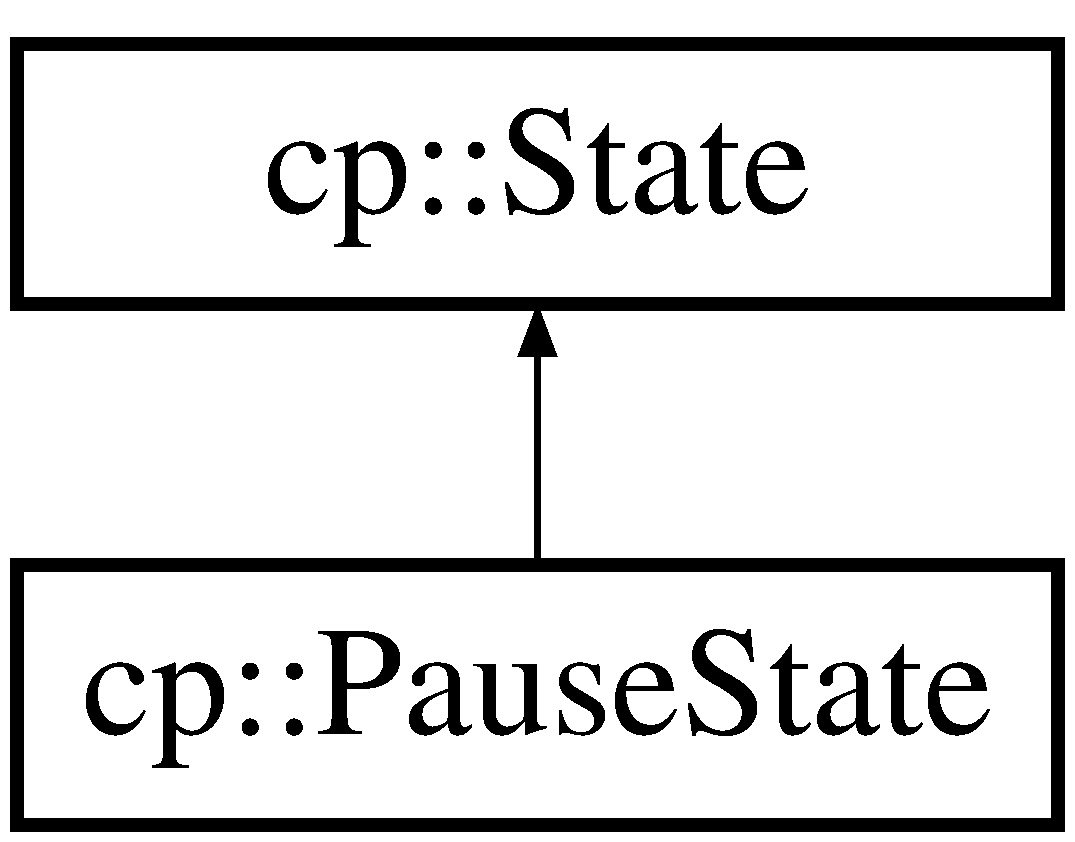
\includegraphics[height=2.000000cm]{classcp_1_1_pause_state}
\end{center}
\end{figure}
\subsection*{Public Member Functions}
\begin{DoxyCompactItemize}
\item 
\mbox{\Hypertarget{classcp_1_1_pause_state_a485171ecabc049352c644935bb1c9f26}\label{classcp_1_1_pause_state_a485171ecabc049352c644935bb1c9f26}} 
{\bfseries Pause\+State} (Game\+Data\+Ref \+\_\+data)
\item 
\mbox{\Hypertarget{classcp_1_1_pause_state_a29233fd0d58f345f0a97781688fa5560}\label{classcp_1_1_pause_state_a29233fd0d58f345f0a97781688fa5560}} 
void {\bfseries init} ()
\item 
\mbox{\Hypertarget{classcp_1_1_pause_state_a8ba6fb40e19af3d9670db732b2768462}\label{classcp_1_1_pause_state_a8ba6fb40e19af3d9670db732b2768462}} 
void {\bfseries handle\+\_\+input} (float delta)
\item 
\mbox{\Hypertarget{classcp_1_1_pause_state_a41f142f0e9aadc49328e9ec2c7b6209c}\label{classcp_1_1_pause_state_a41f142f0e9aadc49328e9ec2c7b6209c}} 
void {\bfseries draw} (float delta)
\item 
\mbox{\Hypertarget{classcp_1_1_pause_state_a4019da6ba2dda3756bd95a767f84e833}\label{classcp_1_1_pause_state_a4019da6ba2dda3756bd95a767f84e833}} 
void {\bfseries update} (float delta)
\end{DoxyCompactItemize}


The documentation for this class was generated from the following files\+:\begin{DoxyCompactItemize}
\item 
include/\+States/Pause\+State.\+hpp\item 
libs/Pause\+State.\+cpp\end{DoxyCompactItemize}

\hypertarget{classcp_1_1_percentage_bar}{}\section{cp\+:\+:Percentage\+Bar Class Reference}
\label{classcp_1_1_percentage_bar}\index{cp\+::\+Percentage\+Bar@{cp\+::\+Percentage\+Bar}}
\subsection*{Public Member Functions}
\begin{DoxyCompactItemize}
\item 
\mbox{\Hypertarget{classcp_1_1_percentage_bar_ab8a2cf28733f06ac05e97b493da3f2f0}\label{classcp_1_1_percentage_bar_ab8a2cf28733f06ac05e97b493da3f2f0}} 
{\bfseries Percentage\+Bar} (Game\+Data\+Ref \+\_\+data)
\item 
\mbox{\Hypertarget{classcp_1_1_percentage_bar_aefcfb21afb5f633a5eb4fca2d5405c63}\label{classcp_1_1_percentage_bar_aefcfb21afb5f633a5eb4fca2d5405c63}} 
void {\bfseries init} (sf\+::\+Vector2f size, sf\+::\+Vector2f position, sf\+::\+Color c1, sf\+::\+Color c2)
\item 
\mbox{\Hypertarget{classcp_1_1_percentage_bar_a15004a48ed290ce7dc017425b554ba33}\label{classcp_1_1_percentage_bar_a15004a48ed290ce7dc017425b554ba33}} 
void {\bfseries draw} ()
\end{DoxyCompactItemize}
\subsection*{Public Attributes}
\begin{DoxyCompactItemize}
\item 
\mbox{\Hypertarget{classcp_1_1_percentage_bar_a1bd6bed09b32268be4fb0a3e93366447}\label{classcp_1_1_percentage_bar_a1bd6bed09b32268be4fb0a3e93366447}} 
float {\bfseries percentage} = 100
\end{DoxyCompactItemize}


The documentation for this class was generated from the following file\+:\begin{DoxyCompactItemize}
\item 
include/Percentage\+Bar.\+hpp\end{DoxyCompactItemize}

\hypertarget{classcp_1_1_player_car}{}\section{cp\+:\+:Player\+Car Class Reference}
\label{classcp_1_1_player_car}\index{cp\+::\+Player\+Car@{cp\+::\+Player\+Car}}
Inheritance diagram for cp\+:\+:Player\+Car\+:\begin{figure}[H]
\begin{center}
\leavevmode
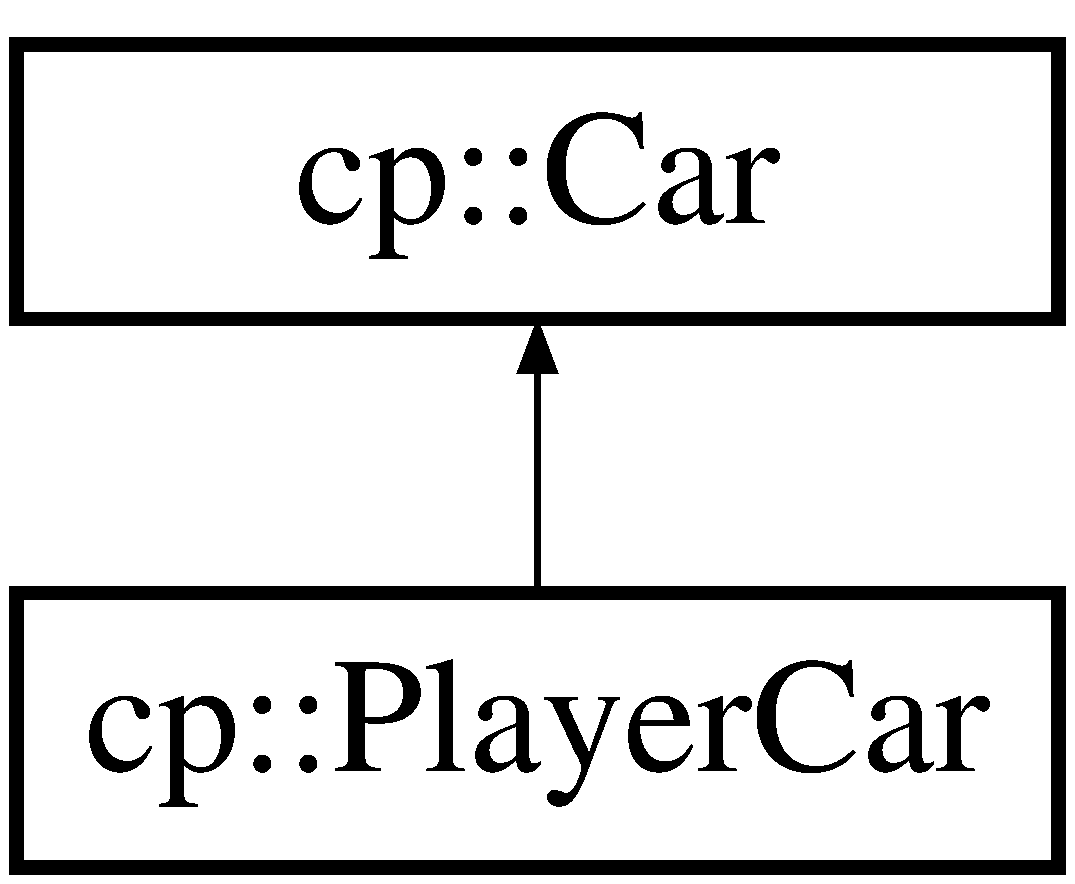
\includegraphics[height=2.000000cm]{classcp_1_1_player_car}
\end{center}
\end{figure}
\subsection*{Public Member Functions}
\begin{DoxyCompactItemize}
\item 
\hyperlink{classcp_1_1_player_car_ae45b93194883e336252dc2c0563f228c}{Player\+Car} (Game\+Data\+Ref \+\_\+data, int \+\_\+car\+\_\+num)
\begin{DoxyCompactList}\small\item\em Construct a new Player \hyperlink{classcp_1_1_car}{Car}\+:\+: Player \hyperlink{classcp_1_1_car}{Car} object. \end{DoxyCompactList}\item 
\mbox{\Hypertarget{classcp_1_1_player_car_ac12da40fef77bb3175fd0ff42a07d4c8}\label{classcp_1_1_player_car_ac12da40fef77bb3175fd0ff42a07d4c8}} 
\hyperlink{classcp_1_1_player_car_ac12da40fef77bb3175fd0ff42a07d4c8}{$\sim$\+Player\+Car} ()
\begin{DoxyCompactList}\small\item\em Destroy the Player \hyperlink{classcp_1_1_car}{Car}\+:\+: Player \hyperlink{classcp_1_1_car}{Car} object. \end{DoxyCompactList}\item 
void \hyperlink{classcp_1_1_player_car_a7c99c7961e6e6301529b65cfdc1104bf}{update\+\_\+car} (float dt, const std\+::vector$<$ \hyperlink{classcp_1_1_line}{Line} $>$ \&lines, float segL)
\begin{DoxyCompactList}\small\item\em Update the car according to it\textquotesingle{}s position and the map. \end{DoxyCompactList}\item 
void \hyperlink{classcp_1_1_player_car_a753b76abce4b6555916ca26919e614f0}{draw\+Sprite} (const \hyperlink{classcp_1_1_line}{Line} \&line)
\begin{DoxyCompactList}\small\item\em Utility function to draw sprites of the car. \end{DoxyCompactList}\item 
\mbox{\Hypertarget{classcp_1_1_player_car_abbb6255a3d76d5b09c119f88abe30235}\label{classcp_1_1_player_car_abbb6255a3d76d5b09c119f88abe30235}} 
void {\bfseries draw\+Using\+Camera} (const \hyperlink{classcp_1_1_camera}{Camera} \&main\+\_\+camera)
\item 
\mbox{\Hypertarget{classcp_1_1_player_car_a377cc2988520e44e4658bc5efdb64fc1}\label{classcp_1_1_player_car_a377cc2988520e44e4658bc5efdb64fc1}} 
void {\bfseries project} (\hyperlink{classcp_1_1_line}{Line} \&line, float camX, float camY, float camZ, float camD)
\item 
void \hyperlink{classcp_1_1_player_car_aa3122b8ea7b398d5b82a5883d052835a}{handle\+\_\+input} (std\+::vector$<$ bool $>$ mask, float dt)
\begin{DoxyCompactList}\small\item\em Provides interface to control the car. \end{DoxyCompactList}\end{DoxyCompactItemize}
\subsection*{Public Attributes}
\begin{DoxyCompactItemize}
\item 
\mbox{\Hypertarget{classcp_1_1_player_car_ad139d2ca2964c27ffe84baa0e2fe4d86}\label{classcp_1_1_player_car_ad139d2ca2964c27ffe84baa0e2fe4d86}} 
float {\bfseries friction} = e\+\_\+max\+\_\+speed.\+z/5
\end{DoxyCompactItemize}


\subsection{Constructor \& Destructor Documentation}
\mbox{\Hypertarget{classcp_1_1_player_car_ae45b93194883e336252dc2c0563f228c}\label{classcp_1_1_player_car_ae45b93194883e336252dc2c0563f228c}} 
\index{cp\+::\+Player\+Car@{cp\+::\+Player\+Car}!Player\+Car@{Player\+Car}}
\index{Player\+Car@{Player\+Car}!cp\+::\+Player\+Car@{cp\+::\+Player\+Car}}
\subsubsection{\texorpdfstring{Player\+Car()}{PlayerCar()}}
{\footnotesize\ttfamily cp\+::\+Player\+Car\+::\+Player\+Car (\begin{DoxyParamCaption}\item[{Game\+Data\+Ref}]{\+\_\+data,  }\item[{int}]{car\+\_\+num }\end{DoxyParamCaption})}



Construct a new Player \hyperlink{classcp_1_1_car}{Car}\+:\+: Player \hyperlink{classcp_1_1_car}{Car} object. 


\begin{DoxyParams}{Parameters}
{\em \+\_\+data} & Pointer Reference to the resources and state machines. \\
\hline
{\em car\+\_\+num} & The sprite number for the car object \\
\hline
\end{DoxyParams}


\subsection{Member Function Documentation}
\mbox{\Hypertarget{classcp_1_1_player_car_a753b76abce4b6555916ca26919e614f0}\label{classcp_1_1_player_car_a753b76abce4b6555916ca26919e614f0}} 
\index{cp\+::\+Player\+Car@{cp\+::\+Player\+Car}!draw\+Sprite@{draw\+Sprite}}
\index{draw\+Sprite@{draw\+Sprite}!cp\+::\+Player\+Car@{cp\+::\+Player\+Car}}
\subsubsection{\texorpdfstring{draw\+Sprite()}{drawSprite()}}
{\footnotesize\ttfamily void cp\+::\+Player\+Car\+::draw\+Sprite (\begin{DoxyParamCaption}\item[{const \hyperlink{classcp_1_1_line}{Line} \&}]{line }\end{DoxyParamCaption})}



Utility function to draw sprites of the car. 


\begin{DoxyParams}{Parameters}
{\em line} & Provides info regarding map scale at the current grid the car is positioned at \\
\hline
\end{DoxyParams}
\mbox{\Hypertarget{classcp_1_1_player_car_aa3122b8ea7b398d5b82a5883d052835a}\label{classcp_1_1_player_car_aa3122b8ea7b398d5b82a5883d052835a}} 
\index{cp\+::\+Player\+Car@{cp\+::\+Player\+Car}!handle\+\_\+input@{handle\+\_\+input}}
\index{handle\+\_\+input@{handle\+\_\+input}!cp\+::\+Player\+Car@{cp\+::\+Player\+Car}}
\subsubsection{\texorpdfstring{handle\+\_\+input()}{handle\_input()}}
{\footnotesize\ttfamily void cp\+::\+Player\+Car\+::handle\+\_\+input (\begin{DoxyParamCaption}\item[{std\+::vector$<$ bool $>$}]{mask,  }\item[{float}]{dt }\end{DoxyParamCaption})}



Provides interface to control the car. 


\begin{DoxyParams}{Parameters}
{\em mask} & Boolean mask indicating the Keyboard inputs. \\
\hline
{\em dt} & Time difference between two handle\+\_\+input call. \\
\hline
\end{DoxyParams}
\mbox{\Hypertarget{classcp_1_1_player_car_a7c99c7961e6e6301529b65cfdc1104bf}\label{classcp_1_1_player_car_a7c99c7961e6e6301529b65cfdc1104bf}} 
\index{cp\+::\+Player\+Car@{cp\+::\+Player\+Car}!update\+\_\+car@{update\+\_\+car}}
\index{update\+\_\+car@{update\+\_\+car}!cp\+::\+Player\+Car@{cp\+::\+Player\+Car}}
\subsubsection{\texorpdfstring{update\+\_\+car()}{update\_car()}}
{\footnotesize\ttfamily void cp\+::\+Player\+Car\+::update\+\_\+car (\begin{DoxyParamCaption}\item[{float}]{dt,  }\item[{const std\+::vector$<$ \hyperlink{classcp_1_1_line}{Line} $>$ \&}]{lines,  }\item[{float}]{segL }\end{DoxyParamCaption})\hspace{0.3cm}{\ttfamily [virtual]}}



Update the car according to it\textquotesingle{}s position and the map. 


\begin{DoxyParams}{Parameters}
{\em dt} & Time difference between two update frames \\
\hline
{\em lines} & provides the map grid info \\
\hline
{\em segL} & Segment line between two grid in the map \\
\hline
\end{DoxyParams}


Implements \hyperlink{classcp_1_1_car}{cp\+::\+Car}.



The documentation for this class was generated from the following files\+:\begin{DoxyCompactItemize}
\item 
include/\+Objects/Player\+Car.\+hpp\item 
libs/\hyperlink{_player_car_8cpp}{Player\+Car.\+cpp}\end{DoxyCompactItemize}

\hypertarget{classcp_1_1_server}{}\section{cp\+:\+:Server Class Reference}
\label{classcp_1_1_server}\index{cp\+::\+Server@{cp\+::\+Server}}
\subsection*{Public Member Functions}
\begin{DoxyCompactItemize}
\item 
\mbox{\Hypertarget{classcp_1_1_server_a01d0cc0ae7adc7594399753f98e90fbc}\label{classcp_1_1_server_a01d0cc0ae7adc7594399753f98e90fbc}} 
\hyperlink{classcp_1_1_server_a01d0cc0ae7adc7594399753f98e90fbc}{Server} ()
\begin{DoxyCompactList}\small\item\em Construct a new \hyperlink{classcp_1_1_server}{Server} object. \end{DoxyCompactList}\item 
ID \hyperlink{classcp_1_1_server_a9a492566ee0efac90c49dec317876311}{get\+\_\+identity} () const
\begin{DoxyCompactList}\small\item\em Get the identity object. \end{DoxyCompactList}\item 
sf\+::\+Tcp\+Socket \& \hyperlink{classcp_1_1_server_aa55a5008f274c0ffd2afa632ec857df7}{get\+\_\+socket} ()
\begin{DoxyCompactList}\small\item\em Get the socket object. \end{DoxyCompactList}\item 
sf\+::\+Socket\+::\+Status \hyperlink{classcp_1_1_server_ae880b305b96776c6c6d38b29a4d3007b}{get\+Last\+Status} () const
\begin{DoxyCompactList}\small\item\em Get the Last Status object. \end{DoxyCompactList}\item 
void \hyperlink{classcp_1_1_server_ae83a84ed4d85c6e432d09013a48392c8}{connect\+\_\+to} (const std\+::string \&ip, int port)
\begin{DoxyCompactList}\small\item\em connect to the specified port and ip \end{DoxyCompactList}\item 
void \hyperlink{classcp_1_1_server_abe6024ffde0c27bb4c1c7a14c206df5a}{send\+\_\+packet} (sf\+::\+Packet \&packet)
\begin{DoxyCompactList}\small\item\em send packet \end{DoxyCompactList}\item 
\mbox{\Hypertarget{classcp_1_1_server_ac815dc5a236bbe5036e139e50c1e8fb4}\label{classcp_1_1_server_ac815dc5a236bbe5036e139e50c1e8fb4}} 
void {\bfseries recieve\+\_\+packet} (sf\+::\+Packet \&packet)
\end{DoxyCompactItemize}
\subsection*{Friends}
\begin{DoxyCompactItemize}
\item 
\hyperlink{classcp_1_1_server}{Server} \& \hyperlink{classcp_1_1_server_a996961461d4083fbb237bce454c42c3f}{operator$<$$<$} (\hyperlink{classcp_1_1_server}{Server} \&server, const key\+\_\+input\+\_\+type \&labelled\+\_\+input)
\begin{DoxyCompactList}\small\item\em Overloaded operator$<$$<$ to send the labelled input. \end{DoxyCompactList}\item 
\hyperlink{classcp_1_1_server}{Server} \& \hyperlink{classcp_1_1_server_a0be043cde5346b18f9fed76e2ae909b7}{operator$>$$>$} (\hyperlink{classcp_1_1_server}{Server} \&server, \hyperlink{classcp_1_1_game_simulator_snap}{Game\+Simulator\+Snap} \&snap)
\begin{DoxyCompactList}\small\item\em Overloaded operator$>$$>$ to recieve Game\+Snaps. \end{DoxyCompactList}\end{DoxyCompactItemize}


\subsection{Member Function Documentation}
\mbox{\Hypertarget{classcp_1_1_server_ae83a84ed4d85c6e432d09013a48392c8}\label{classcp_1_1_server_ae83a84ed4d85c6e432d09013a48392c8}} 
\index{cp\+::\+Server@{cp\+::\+Server}!connect\+\_\+to@{connect\+\_\+to}}
\index{connect\+\_\+to@{connect\+\_\+to}!cp\+::\+Server@{cp\+::\+Server}}
\subsubsection{\texorpdfstring{connect\+\_\+to()}{connect\_to()}}
{\footnotesize\ttfamily void cp\+::\+Server\+::connect\+\_\+to (\begin{DoxyParamCaption}\item[{const std\+::string \&}]{ip,  }\item[{int}]{port }\end{DoxyParamCaption})\hspace{0.3cm}{\ttfamily [inline]}}



connect to the specified port and ip 


\begin{DoxyParams}{Parameters}
{\em ip} & IP of the server. \\
\hline
{\em port} & P\+O\+RT of the server. \\
\hline
\end{DoxyParams}
\mbox{\Hypertarget{classcp_1_1_server_a9a492566ee0efac90c49dec317876311}\label{classcp_1_1_server_a9a492566ee0efac90c49dec317876311}} 
\index{cp\+::\+Server@{cp\+::\+Server}!get\+\_\+identity@{get\+\_\+identity}}
\index{get\+\_\+identity@{get\+\_\+identity}!cp\+::\+Server@{cp\+::\+Server}}
\subsubsection{\texorpdfstring{get\+\_\+identity()}{get\_identity()}}
{\footnotesize\ttfamily ID cp\+::\+Server\+::get\+\_\+identity (\begin{DoxyParamCaption}{ }\end{DoxyParamCaption}) const\hspace{0.3cm}{\ttfamily [inline]}}



Get the identity object. 

\begin{DoxyReturn}{Returns}
ID id of the \hyperlink{classcp_1_1_server}{Server}. 
\end{DoxyReturn}
\mbox{\Hypertarget{classcp_1_1_server_aa55a5008f274c0ffd2afa632ec857df7}\label{classcp_1_1_server_aa55a5008f274c0ffd2afa632ec857df7}} 
\index{cp\+::\+Server@{cp\+::\+Server}!get\+\_\+socket@{get\+\_\+socket}}
\index{get\+\_\+socket@{get\+\_\+socket}!cp\+::\+Server@{cp\+::\+Server}}
\subsubsection{\texorpdfstring{get\+\_\+socket()}{get\_socket()}}
{\footnotesize\ttfamily sf\+::\+Tcp\+Socket\& cp\+::\+Server\+::get\+\_\+socket (\begin{DoxyParamCaption}{ }\end{DoxyParamCaption})\hspace{0.3cm}{\ttfamily [inline]}}



Get the socket object. 

\begin{DoxyReturn}{Returns}
sf\+::\+Tcp\+Socket\& I\+Nternal handle of the socket. 
\end{DoxyReturn}
\mbox{\Hypertarget{classcp_1_1_server_ae880b305b96776c6c6d38b29a4d3007b}\label{classcp_1_1_server_ae880b305b96776c6c6d38b29a4d3007b}} 
\index{cp\+::\+Server@{cp\+::\+Server}!get\+Last\+Status@{get\+Last\+Status}}
\index{get\+Last\+Status@{get\+Last\+Status}!cp\+::\+Server@{cp\+::\+Server}}
\subsubsection{\texorpdfstring{get\+Last\+Status()}{getLastStatus()}}
{\footnotesize\ttfamily sf\+::\+Socket\+::\+Status cp\+::\+Server\+::get\+Last\+Status (\begin{DoxyParamCaption}{ }\end{DoxyParamCaption}) const\hspace{0.3cm}{\ttfamily [inline]}}



Get the Last Status object. 

\begin{DoxyReturn}{Returns}
sf\+::\+Socket\+::\+Status Status of the last function call to recieve/send. 
\end{DoxyReturn}
\mbox{\Hypertarget{classcp_1_1_server_abe6024ffde0c27bb4c1c7a14c206df5a}\label{classcp_1_1_server_abe6024ffde0c27bb4c1c7a14c206df5a}} 
\index{cp\+::\+Server@{cp\+::\+Server}!send\+\_\+packet@{send\+\_\+packet}}
\index{send\+\_\+packet@{send\+\_\+packet}!cp\+::\+Server@{cp\+::\+Server}}
\subsubsection{\texorpdfstring{send\+\_\+packet()}{send\_packet()}}
{\footnotesize\ttfamily void cp\+::\+Server\+::send\+\_\+packet (\begin{DoxyParamCaption}\item[{sf\+::\+Packet \&}]{packet }\end{DoxyParamCaption})\hspace{0.3cm}{\ttfamily [inline]}}



send packet 


\begin{DoxyParams}{Parameters}
{\em packet} & \\
\hline
\end{DoxyParams}


\subsection{Friends And Related Function Documentation}
\mbox{\Hypertarget{classcp_1_1_server_a996961461d4083fbb237bce454c42c3f}\label{classcp_1_1_server_a996961461d4083fbb237bce454c42c3f}} 
\index{cp\+::\+Server@{cp\+::\+Server}!operator$<$$<$@{operator$<$$<$}}
\index{operator$<$$<$@{operator$<$$<$}!cp\+::\+Server@{cp\+::\+Server}}
\subsubsection{\texorpdfstring{operator$<$$<$}{operator<<}}
{\footnotesize\ttfamily \hyperlink{classcp_1_1_server}{Server}\& operator$<$$<$ (\begin{DoxyParamCaption}\item[{\hyperlink{classcp_1_1_server}{Server} \&}]{server,  }\item[{const key\+\_\+input\+\_\+type \&}]{labelled\+\_\+input }\end{DoxyParamCaption})\hspace{0.3cm}{\ttfamily [friend]}}



Overloaded operator$<$$<$ to send the labelled input. 


\begin{DoxyParams}{Parameters}
{\em server} & The server that you want to send the labelled input to. \\
\hline
{\em labelled\+\_\+input} & The labelled input to send. \\
\hline
\end{DoxyParams}
\begin{DoxyReturn}{Returns}
\hyperlink{classcp_1_1_server}{Server}\& Returns back the server reference. 
\end{DoxyReturn}
\mbox{\Hypertarget{classcp_1_1_server_a0be043cde5346b18f9fed76e2ae909b7}\label{classcp_1_1_server_a0be043cde5346b18f9fed76e2ae909b7}} 
\index{cp\+::\+Server@{cp\+::\+Server}!operator$>$$>$@{operator$>$$>$}}
\index{operator$>$$>$@{operator$>$$>$}!cp\+::\+Server@{cp\+::\+Server}}
\subsubsection{\texorpdfstring{operator$>$$>$}{operator>>}}
{\footnotesize\ttfamily \hyperlink{classcp_1_1_server}{Server}\& operator$>$$>$ (\begin{DoxyParamCaption}\item[{\hyperlink{classcp_1_1_server}{Server} \&}]{server,  }\item[{\hyperlink{classcp_1_1_game_simulator_snap}{Game\+Simulator\+Snap} \&}]{snap }\end{DoxyParamCaption})\hspace{0.3cm}{\ttfamily [friend]}}



Overloaded operator$>$$>$ to recieve Game\+Snaps. 


\begin{DoxyParams}{Parameters}
{\em server} & The server that you want to recieve snap from. \\
\hline
{\em snap} & The snap reference for getting incoming snap. \\
\hline
\end{DoxyParams}
\begin{DoxyReturn}{Returns}
\hyperlink{classcp_1_1_server}{Server}\& Returns back the server. 
\end{DoxyReturn}


The documentation for this class was generated from the following file\+:\begin{DoxyCompactItemize}
\item 
include/\+Network/\hyperlink{_server_8hpp}{Server.\+hpp}\end{DoxyCompactItemize}

\hypertarget{classcp_1_1_server_room}{}\section{cp\+:\+:Server\+Room Class Reference}
\label{classcp_1_1_server_room}\index{cp\+::\+Server\+Room@{cp\+::\+Server\+Room}}
Inheritance diagram for cp\+:\+:Server\+Room\+:\begin{figure}[H]
\begin{center}
\leavevmode
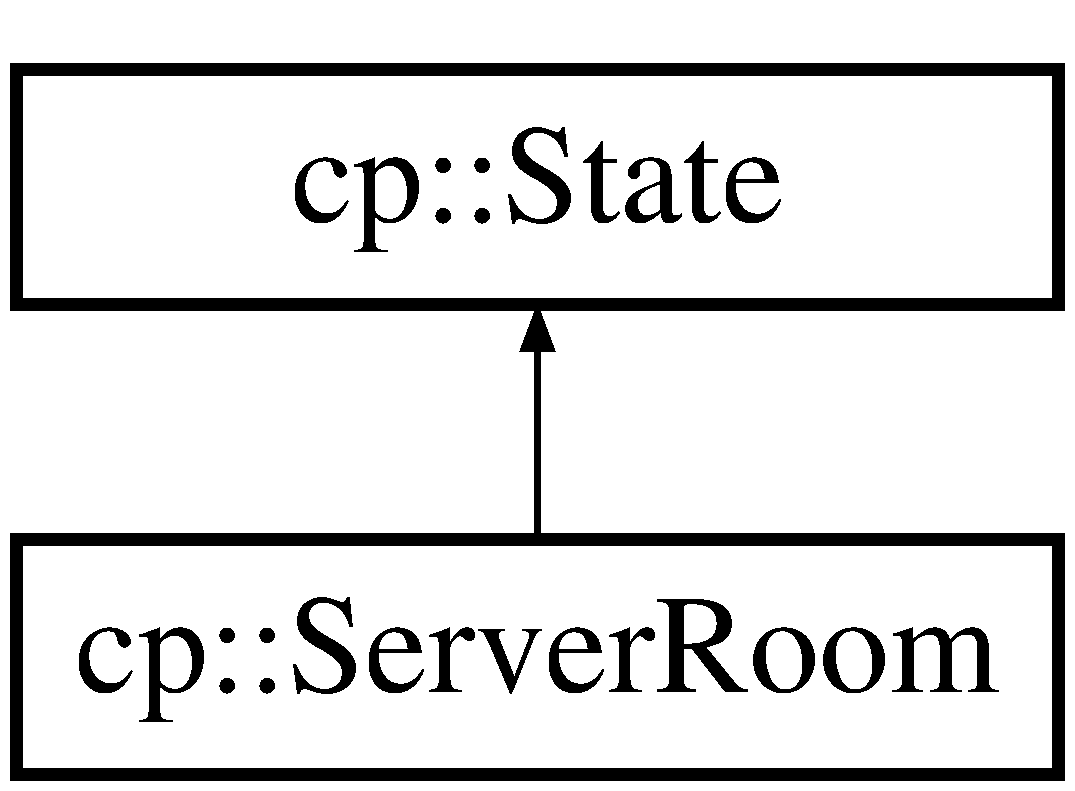
\includegraphics[height=2.000000cm]{classcp_1_1_server_room}
\end{center}
\end{figure}
\subsection*{Public Member Functions}
\begin{DoxyCompactItemize}
\item 
\mbox{\Hypertarget{classcp_1_1_server_room_ac11f8f51d5242b796f79e042b7918541}\label{classcp_1_1_server_room_ac11f8f51d5242b796f79e042b7918541}} 
{\bfseries Server\+Room} (Game\+Data\+Ref \+\_\+data)
\item 
\mbox{\Hypertarget{classcp_1_1_server_room_adc9e2fe2c4a6e59d7b33744470b71b85}\label{classcp_1_1_server_room_adc9e2fe2c4a6e59d7b33744470b71b85}} 
void {\bfseries init} ()
\item 
\mbox{\Hypertarget{classcp_1_1_server_room_a0330143a408d7956e746795c21c143ff}\label{classcp_1_1_server_room_a0330143a408d7956e746795c21c143ff}} 
virtual void {\bfseries handle\+\_\+input} (float delta)
\item 
\mbox{\Hypertarget{classcp_1_1_server_room_a561b8c66d9cd87e59c5f309d45bad6d1}\label{classcp_1_1_server_room_a561b8c66d9cd87e59c5f309d45bad6d1}} 
virtual void {\bfseries update} (float delta)
\item 
\mbox{\Hypertarget{classcp_1_1_server_room_af27b01b2d8e93b5d14df8a60b9220e79}\label{classcp_1_1_server_room_af27b01b2d8e93b5d14df8a60b9220e79}} 
virtual void {\bfseries draw} (float delta)
\item 
\mbox{\Hypertarget{classcp_1_1_server_room_af645f2f2b9bb1cd10b60df3b2fb4f596}\label{classcp_1_1_server_room_af645f2f2b9bb1cd10b60df3b2fb4f596}} 
virtual void {\bfseries pause} ()
\item 
\mbox{\Hypertarget{classcp_1_1_server_room_ae3f282bcaf70b6ab8b5b6e2f3e05a66b}\label{classcp_1_1_server_room_ae3f282bcaf70b6ab8b5b6e2f3e05a66b}} 
virtual void {\bfseries resume} ()
\end{DoxyCompactItemize}


The documentation for this class was generated from the following file\+:\begin{DoxyCompactItemize}
\item 
include/\+Network/\hyperlink{_server_room_8hpp}{Server\+Room.\+hpp}\end{DoxyCompactItemize}

\hypertarget{classcp_1_1_server_state}{}\section{cp\+:\+:Server\+State Class Reference}
\label{classcp_1_1_server_state}\index{cp\+::\+Server\+State@{cp\+::\+Server\+State}}


\hyperlink{classcp_1_1_server_state}{Server\+State} is the state where network updates takes place. It is the game simulator which simulates the game and then update the relevant data over the network.  




{\ttfamily \#include $<$Server\+State.\+hpp$>$}

Inheritance diagram for cp\+:\+:Server\+State\+:\begin{figure}[H]
\begin{center}
\leavevmode
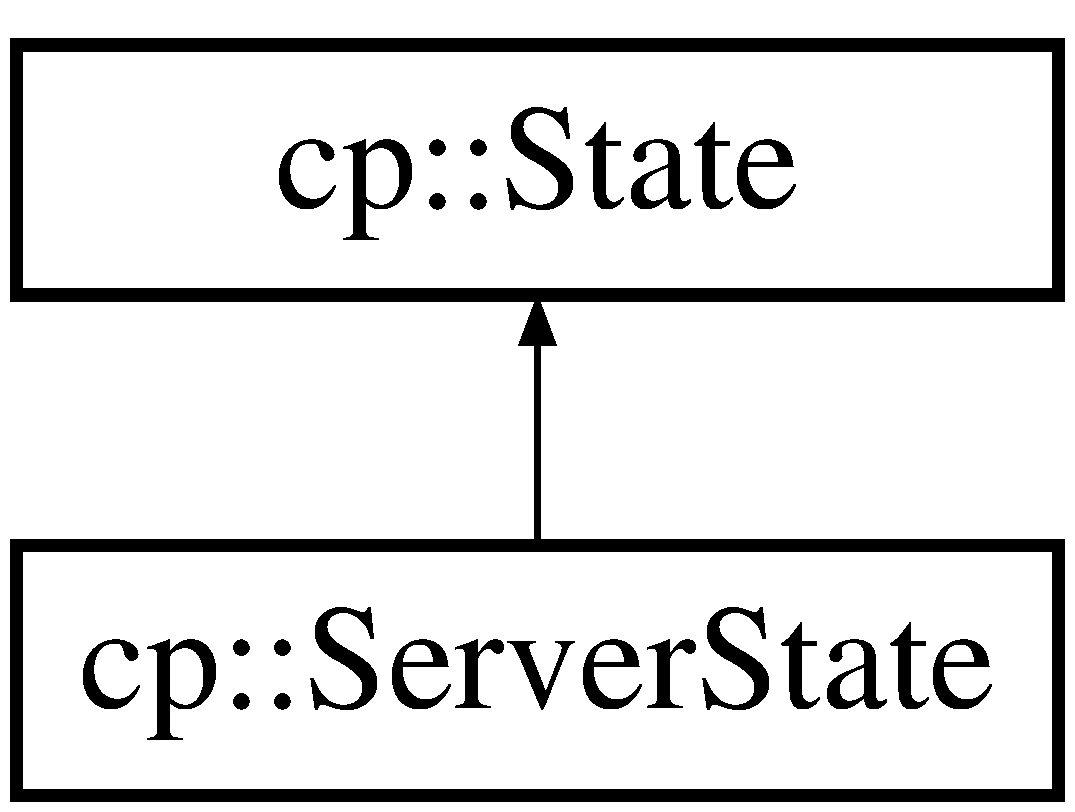
\includegraphics[height=2.000000cm]{classcp_1_1_server_state}
\end{center}
\end{figure}
\subsection*{Public Member Functions}
\begin{DoxyCompactItemize}
\item 
\mbox{\Hypertarget{classcp_1_1_server_state_aa468fbc97117dc95b490529ab89b5998}\label{classcp_1_1_server_state_aa468fbc97117dc95b490529ab89b5998}} 
{\bfseries Server\+State} (Game\+Data\+Ref \+\_\+data, std\+::set$<$ Tcp\+Client\+\_\+ptr $>$ clients)
\item 
\mbox{\Hypertarget{classcp_1_1_server_state_a50dff11b2bc3defc5b915dc23cf3facb}\label{classcp_1_1_server_state_a50dff11b2bc3defc5b915dc23cf3facb}} 
virtual void {\bfseries handle\+\_\+input} (float delta)
\item 
\mbox{\Hypertarget{classcp_1_1_server_state_a07143b5e396a15b32b8cb3896c0e7239}\label{classcp_1_1_server_state_a07143b5e396a15b32b8cb3896c0e7239}} 
virtual void {\bfseries update} (float delta)
\item 
\mbox{\Hypertarget{classcp_1_1_server_state_ab43314cff0977d35aacdbf781cefff8c}\label{classcp_1_1_server_state_ab43314cff0977d35aacdbf781cefff8c}} 
virtual void {\bfseries draw} (float delta)
\item 
\mbox{\Hypertarget{classcp_1_1_server_state_a84a56ac8094e1b75551b170411af195f}\label{classcp_1_1_server_state_a84a56ac8094e1b75551b170411af195f}} 
virtual void {\bfseries pause} ()
\item 
\mbox{\Hypertarget{classcp_1_1_server_state_a7dd7b18f6b378e907fd286ba20bc9e11}\label{classcp_1_1_server_state_a7dd7b18f6b378e907fd286ba20bc9e11}} 
virtual void {\bfseries resume} ()
\item 
\mbox{\Hypertarget{classcp_1_1_server_state_a54d67dcec1e8a1dad2fd94259dab7fd6}\label{classcp_1_1_server_state_a54d67dcec1e8a1dad2fd94259dab7fd6}} 
virtual void {\bfseries init} ()
\end{DoxyCompactItemize}


\subsection{Detailed Description}
\hyperlink{classcp_1_1_server_state}{Server\+State} is the state where network updates takes place. It is the game simulator which simulates the game and then update the relevant data over the network. 

The documentation for this class was generated from the following files\+:\begin{DoxyCompactItemize}
\item 
include/\+States/\hyperlink{_server_state_8hpp}{Server\+State.\+hpp}\item 
libs/Server\+State.\+cpp\end{DoxyCompactItemize}

\hypertarget{classcp_1_1_splash_state}{}\section{cp\+:\+:Splash\+State Class Reference}
\label{classcp_1_1_splash_state}\index{cp\+::\+Splash\+State@{cp\+::\+Splash\+State}}
Inheritance diagram for cp\+:\+:Splash\+State\+:\begin{figure}[H]
\begin{center}
\leavevmode
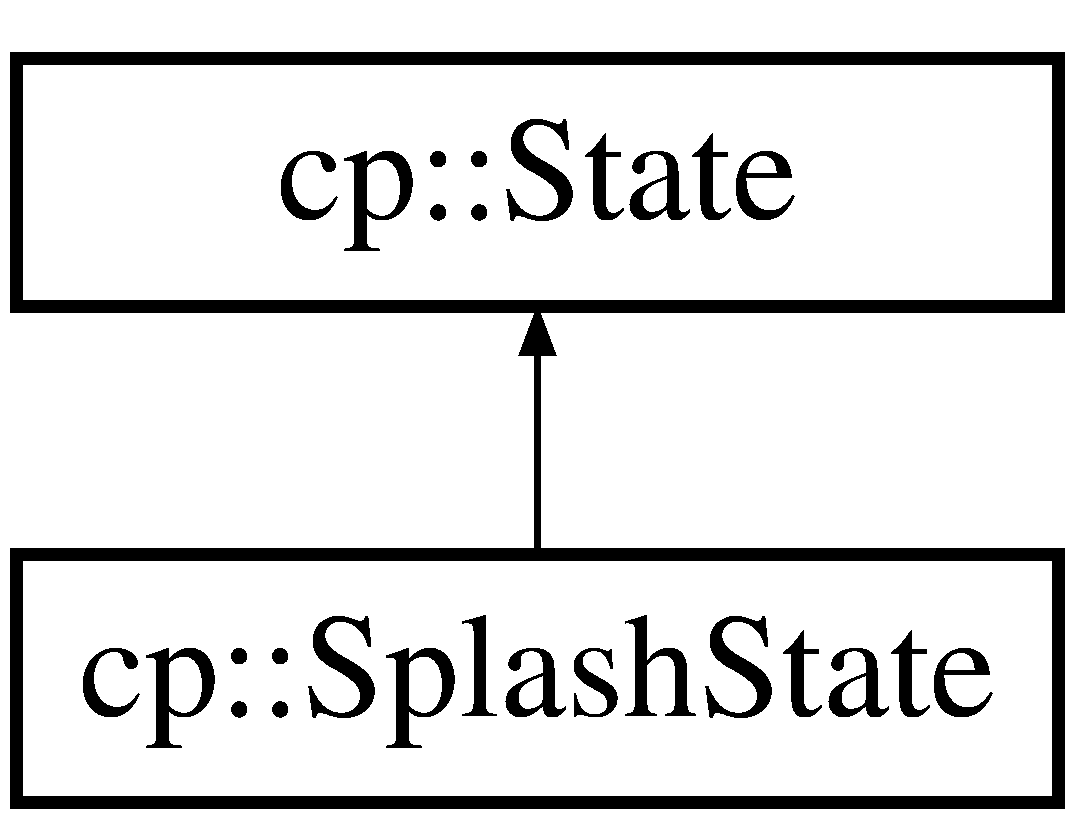
\includegraphics[height=2.000000cm]{classcp_1_1_splash_state}
\end{center}
\end{figure}
\subsection*{Public Member Functions}
\begin{DoxyCompactItemize}
\item 
\mbox{\Hypertarget{classcp_1_1_splash_state_a13c8bbda231f1a6b61a7b48f5d5d78fa}\label{classcp_1_1_splash_state_a13c8bbda231f1a6b61a7b48f5d5d78fa}} 
{\bfseries Splash\+State} (Game\+Data\+Ref \+\_\+data)
\item 
\mbox{\Hypertarget{classcp_1_1_splash_state_a04c76eeff72330b606761cc3cfc02138}\label{classcp_1_1_splash_state_a04c76eeff72330b606761cc3cfc02138}} 
void {\bfseries init} ()
\item 
\mbox{\Hypertarget{classcp_1_1_splash_state_a38939d73fbb4e3b6fa377fcc8fbc1dae}\label{classcp_1_1_splash_state_a38939d73fbb4e3b6fa377fcc8fbc1dae}} 
void {\bfseries handle\+\_\+input} (float delta)
\item 
\mbox{\Hypertarget{classcp_1_1_splash_state_a4ff5d8ca42efef65c8f572a29af89ec0}\label{classcp_1_1_splash_state_a4ff5d8ca42efef65c8f572a29af89ec0}} 
void {\bfseries draw} (float delta)
\item 
\mbox{\Hypertarget{classcp_1_1_splash_state_a3f906e4b3904c2813e18a63000b97ac8}\label{classcp_1_1_splash_state_a3f906e4b3904c2813e18a63000b97ac8}} 
void {\bfseries update} (float delta)
\end{DoxyCompactItemize}


The documentation for this class was generated from the following files\+:\begin{DoxyCompactItemize}
\item 
include/\+States/Splash\+State.\+hpp\item 
libs/Splash\+State.\+cpp\end{DoxyCompactItemize}

\hypertarget{classcp_1_1_state}{}\section{cp\+:\+:State Class Reference}
\label{classcp_1_1_state}\index{cp\+::\+State@{cp\+::\+State}}
Inheritance diagram for cp\+:\+:State\+:\begin{figure}[H]
\begin{center}
\leavevmode
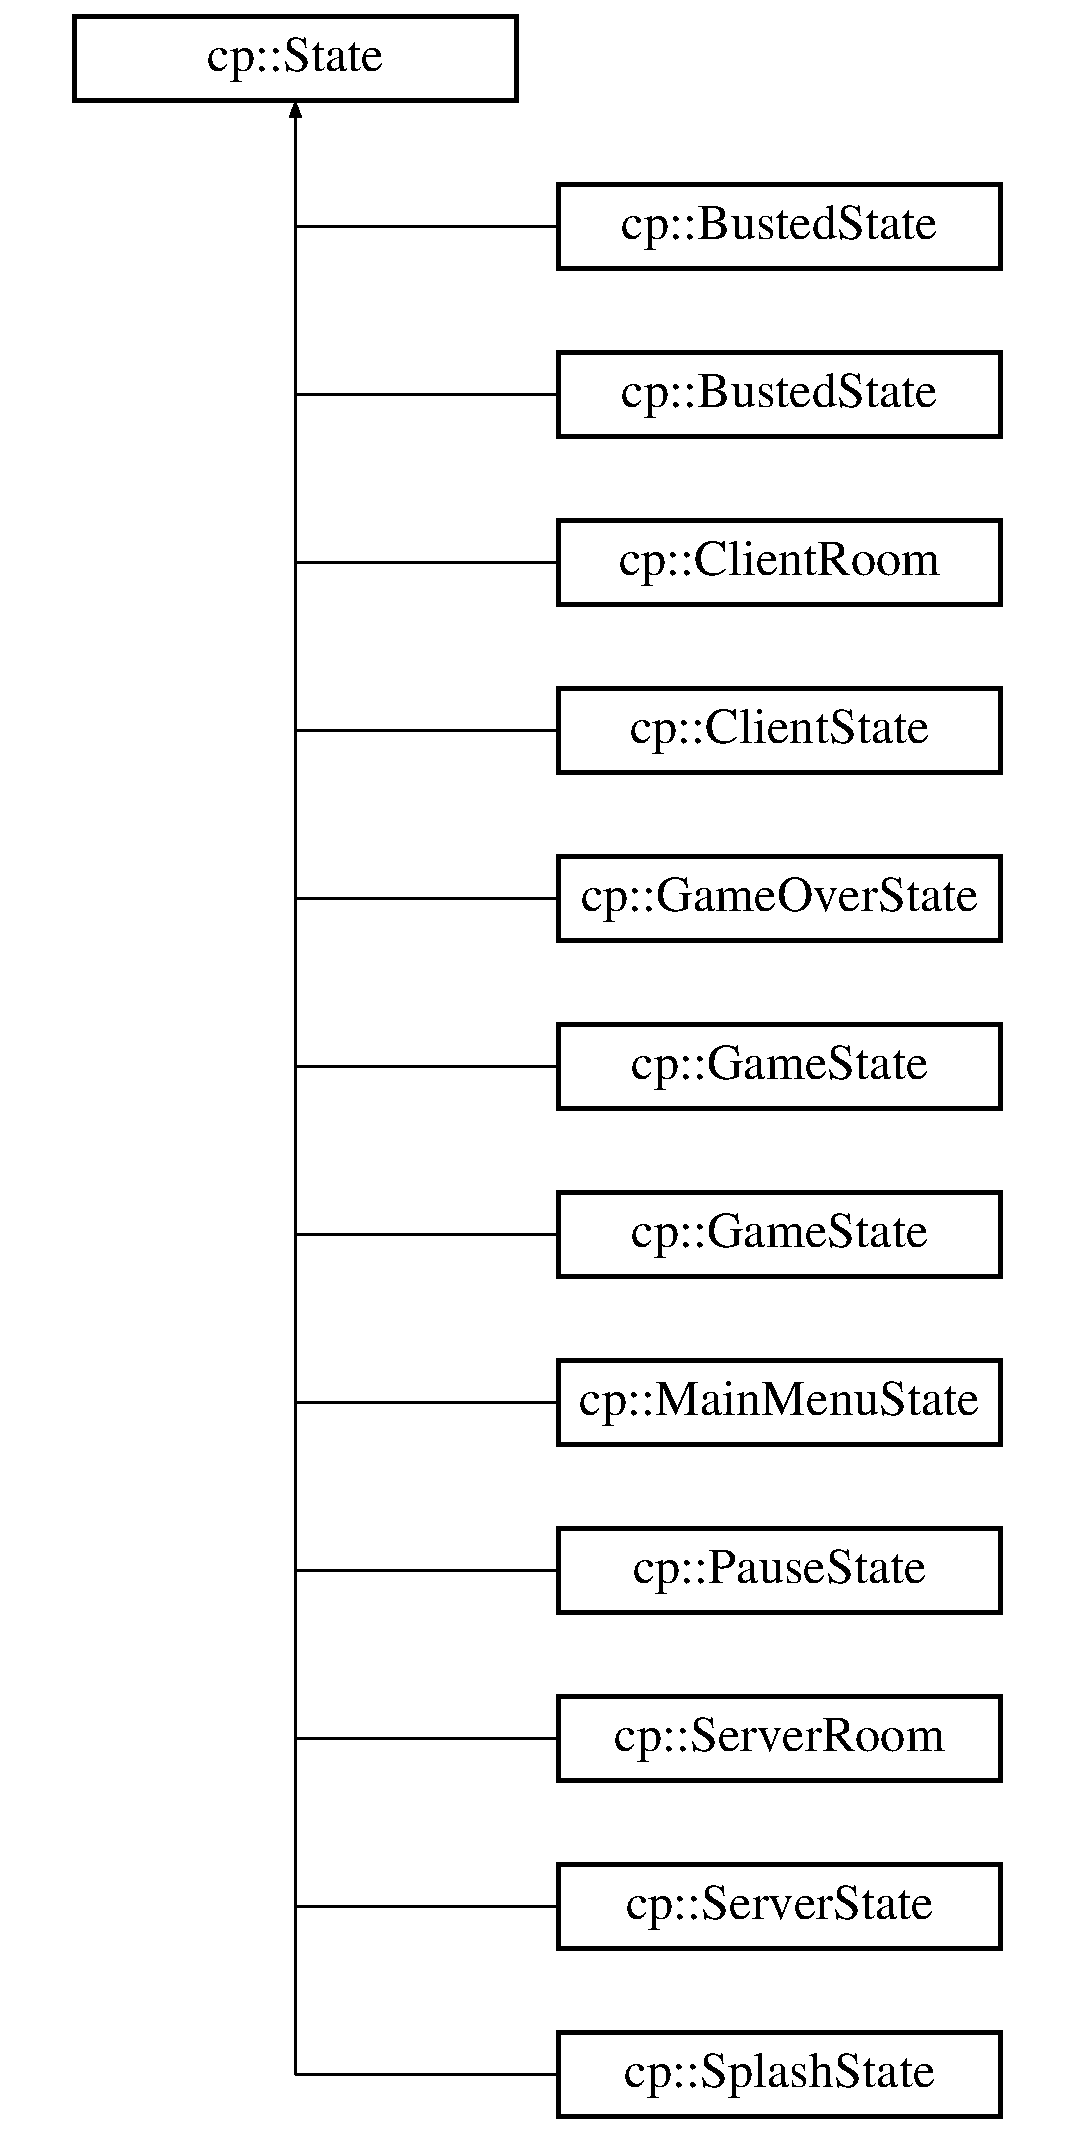
\includegraphics[height=12.000000cm]{classcp_1_1_state}
\end{center}
\end{figure}
\subsection*{Public Member Functions}
\begin{DoxyCompactItemize}
\item 
\mbox{\Hypertarget{classcp_1_1_state_a680b39b3b4ad5c48976f92ec0fc24583}\label{classcp_1_1_state_a680b39b3b4ad5c48976f92ec0fc24583}} 
virtual void {\bfseries init} ()=0
\item 
\mbox{\Hypertarget{classcp_1_1_state_a368c6323f68a53faaf3cbcbe184daf9a}\label{classcp_1_1_state_a368c6323f68a53faaf3cbcbe184daf9a}} 
virtual void {\bfseries handle\+\_\+input} (float delta)=0
\item 
\mbox{\Hypertarget{classcp_1_1_state_a035c6962af689234630033bd3741ea1e}\label{classcp_1_1_state_a035c6962af689234630033bd3741ea1e}} 
virtual void {\bfseries update} (float delta)=0
\item 
\mbox{\Hypertarget{classcp_1_1_state_a4cee56e000513cd065393cdc297a8256}\label{classcp_1_1_state_a4cee56e000513cd065393cdc297a8256}} 
virtual void {\bfseries draw} (float delta)=0
\item 
\mbox{\Hypertarget{classcp_1_1_state_a86eeda9796d7086669bc4275c3f9f98c}\label{classcp_1_1_state_a86eeda9796d7086669bc4275c3f9f98c}} 
virtual void {\bfseries pause} ()
\item 
\mbox{\Hypertarget{classcp_1_1_state_afac74aaab36c734bdb9da377018a4ae4}\label{classcp_1_1_state_afac74aaab36c734bdb9da377018a4ae4}} 
virtual void {\bfseries resume} ()
\end{DoxyCompactItemize}


The documentation for this class was generated from the following file\+:\begin{DoxyCompactItemize}
\item 
include/\+States/State.\+hpp\end{DoxyCompactItemize}

\hypertarget{classcp_1_1_state_machine}{}\section{cp\+:\+:State\+Machine Class Reference}
\label{classcp_1_1_state_machine}\index{cp\+::\+State\+Machine@{cp\+::\+State\+Machine}}
\subsection*{Public Member Functions}
\begin{DoxyCompactItemize}
\item 
\mbox{\Hypertarget{classcp_1_1_state_machine_a21eee65ecdafdf86890fafdb1296dd84}\label{classcp_1_1_state_machine_a21eee65ecdafdf86890fafdb1296dd84}} 
void {\bfseries add\+\_\+state} (State\+Ref new\+\_\+state, bool is\+\_\+replacing=true)
\item 
\mbox{\Hypertarget{classcp_1_1_state_machine_af9149160433276096ad722fd44f7193e}\label{classcp_1_1_state_machine_af9149160433276096ad722fd44f7193e}} 
void {\bfseries remove\+\_\+state} ()
\item 
\mbox{\Hypertarget{classcp_1_1_state_machine_afbb74374e2603291b5bc639e91508cce}\label{classcp_1_1_state_machine_afbb74374e2603291b5bc639e91508cce}} 
void {\bfseries process\+\_\+state\+\_\+change} ()
\item 
\mbox{\Hypertarget{classcp_1_1_state_machine_abd0b0c0af69f4368b9fcad9ff0f422af}\label{classcp_1_1_state_machine_abd0b0c0af69f4368b9fcad9ff0f422af}} 
State\+Ref \& {\bfseries get\+\_\+active\+\_\+state} ()
\end{DoxyCompactItemize}


The documentation for this class was generated from the following files\+:\begin{DoxyCompactItemize}
\item 
include/\+States/State\+Machine.\+hpp\item 
libs/State\+Machine.\+cpp\end{DoxyCompactItemize}

\chapter{File Documentation}
\hypertarget{_client_8hpp}{}\section{include/\+Network/\+Client.hpp File Reference}
\label{_client_8hpp}\index{include/\+Network/\+Client.\+hpp@{include/\+Network/\+Client.\+hpp}}


Client class refers to a another pc connected over network.  


{\ttfamily \#include $<$string$>$}\newline
{\ttfamily \#include \char`\"{}States/\+Game\+Simulator.\+hpp\char`\"{}}\newline
{\ttfamily \#include \char`\"{}S\+F\+M\+L/\+Network.\+hpp\char`\"{}}\newline
\subsection*{Classes}
\begin{DoxyCompactItemize}
\item 
class \hyperlink{classcp_1_1_client}{cp\+::\+Client}
\end{DoxyCompactItemize}


\subsection{Detailed Description}
Client class refers to a another pc connected over network. 

\begin{DoxyAuthor}{Author}
Anjani Kumar (\href{mailto:cs17btech11002@iith.ac.in}{\tt cs17btech11002@iith.\+ac.\+in}) 
\end{DoxyAuthor}
\begin{DoxyVersion}{Version}
0.\+1 
\end{DoxyVersion}
\begin{DoxyDate}{Date}
2019-\/02-\/26
\end{DoxyDate}
\begin{DoxyCopyright}{Copyright}
Copyright (c) 2019 
\end{DoxyCopyright}

\hypertarget{_client_room_8hpp}{}\section{include/\+Network/\+Client\+Room.hpp File Reference}
\label{_client_room_8hpp}\index{include/\+Network/\+Client\+Room.\+hpp@{include/\+Network/\+Client\+Room.\+hpp}}


The client room that is displayed on client\textquotesingle{}s computer just before online game play.  


{\ttfamily \#include \char`\"{}States/\+State.\+hpp\char`\"{}}\newline
{\ttfamily \#include \char`\"{}Game.\+hpp\char`\"{}}\newline
{\ttfamily \#include \char`\"{}Network/\+Server.\+hpp\char`\"{}}\newline
{\ttfamily \#include $<$iostream$>$}\newline
{\ttfamily \#include $<$fstream$>$}\newline
{\ttfamily \#include $<$cstring$>$}\newline
{\ttfamily \#include $<$memory$>$}\newline
{\ttfamily \#include \char`\"{}States/\+Client\+State.\+hpp\char`\"{}}\newline
\subsection*{Classes}
\begin{DoxyCompactItemize}
\item 
class \hyperlink{classcp_1_1_client_room}{cp\+::\+Client\+Room}
\end{DoxyCompactItemize}


\subsection{Detailed Description}
The client room that is displayed on client\textquotesingle{}s computer just before online game play. 

\begin{DoxyAuthor}{Author}
Anjani Kumar (\href{mailto:cs17btech11002@iith.ac.in}{\tt cs17btech11002@iith.\+ac.\+in}) 
\end{DoxyAuthor}
\begin{DoxyVersion}{Version}
0.\+1 
\end{DoxyVersion}
\begin{DoxyDate}{Date}
2019-\/02-\/28
\end{DoxyDate}
\begin{DoxyCopyright}{Copyright}
Copyright (c) 2019 
\end{DoxyCopyright}

\hypertarget{_server_8hpp}{}\section{include/\+Network/\+Server.hpp File Reference}
\label{_server_8hpp}\index{include/\+Network/\+Server.\+hpp@{include/\+Network/\+Server.\+hpp}}


Server class that handles the data sending over the network.  


{\ttfamily \#include \char`\"{}States/\+Game\+Simulator.\+hpp\char`\"{}}\newline
\subsection*{Classes}
\begin{DoxyCompactItemize}
\item 
class \hyperlink{classcp_1_1_server}{cp\+::\+Server}
\end{DoxyCompactItemize}


\subsection{Detailed Description}
Server class that handles the data sending over the network. 

\begin{DoxyAuthor}{Author}
Anjani Kumar (\href{mailto:cs17btech11002@iith.ac.in}{\tt cs17btech11002@iith.\+ac.\+in}) 
\end{DoxyAuthor}
\begin{DoxyVersion}{Version}
0.\+1 
\end{DoxyVersion}
\begin{DoxyDate}{Date}
2019-\/02-\/26
\end{DoxyDate}
\begin{DoxyCopyright}{Copyright}
Copyright (c) 2019 
\end{DoxyCopyright}

\hypertarget{_server_room_8hpp}{}\section{include/\+Network/\+Server\+Room.hpp File Reference}
\label{_server_room_8hpp}\index{include/\+Network/\+Server\+Room.\+hpp@{include/\+Network/\+Server\+Room.\+hpp}}


Simple Server room displayed before Online Play Starts.  


{\ttfamily \#include \char`\"{}States/\+State.\+hpp\char`\"{}}\newline
{\ttfamily \#include \char`\"{}Game.\+hpp\char`\"{}}\newline
{\ttfamily \#include \char`\"{}Network/\+Client.\+hpp\char`\"{}}\newline
{\ttfamily \#include $<$iostream$>$}\newline
{\ttfamily \#include $<$cstring$>$}\newline
{\ttfamily \#include \char`\"{}States/\+Server\+State.\+hpp\char`\"{}}\newline
{\ttfamily \#include $<$set$>$}\newline
{\ttfamily \#include $<$fstream$>$}\newline
{\ttfamily \#include $<$memory$>$}\newline
\subsection*{Classes}
\begin{DoxyCompactItemize}
\item 
class \hyperlink{classcp_1_1_server_room}{cp\+::\+Server\+Room}
\end{DoxyCompactItemize}


\subsection{Detailed Description}
Simple Server room displayed before Online Play Starts. 

\begin{DoxyAuthor}{Author}
Anjani (\href{mailto:cs17btech11002@iith.ac.in}{\tt cs17btech11002@iith.\+ac.\+in}) 
\end{DoxyAuthor}
\begin{DoxyVersion}{Version}
0.\+1 
\end{DoxyVersion}
\begin{DoxyDate}{Date}
2019-\/02-\/27
\end{DoxyDate}
\begin{DoxyCopyright}{Copyright}
Copyright (c) 2019 
\end{DoxyCopyright}

\hypertarget{_object_pool_8hpp}{}\section{include/\+Object\+Pool.hpp File Reference}
\label{_object_pool_8hpp}\index{include/\+Object\+Pool.\+hpp@{include/\+Object\+Pool.\+hpp}}
{\ttfamily \#include $<$S\+F\+M\+L/\+Graphics.\+hpp$>$}\newline
{\ttfamily \#include $<$list$>$}\newline
{\ttfamily \#include $<$iostream$>$}\newline
{\ttfamily \#include $<$memory$>$}\newline
{\ttfamily \#include \char`\"{}Objects/\+Car.\+hpp\char`\"{}}\newline
{\ttfamily \#include \char`\"{}Objects/\+Bot.\+hpp\char`\"{}}\newline
{\ttfamily \#include \char`\"{}Game.\+hpp\char`\"{}}\newline
{\ttfamily \#include \char`\"{}Objects/\+Bullet.\+hpp\char`\"{}}\newline
\subsection*{Classes}
\begin{DoxyCompactItemize}
\item 
class \hyperlink{classcp_1_1_object_pool}{cp\+::\+Object\+Pool$<$ T $>$}
\end{DoxyCompactItemize}


\subsection{Detailed Description}
\begin{DoxyAuthor}{Author}
your name (\href{mailto:you@domain.com}{\tt you@domain.\+com}) 
\end{DoxyAuthor}
\begin{DoxyVersion}{Version}
0.\+1 
\end{DoxyVersion}
\begin{DoxyDate}{Date}
2019-\/02-\/28
\end{DoxyDate}
\begin{DoxyCopyright}{Copyright}
Copyright (c) 2019 
\end{DoxyCopyright}

\hypertarget{_client_state_8hpp}{}\section{include/\+States/\+Client\+State.hpp File Reference}
\label{_client_state_8hpp}\index{include/\+States/\+Client\+State.\+hpp@{include/\+States/\+Client\+State.\+hpp}}


Handles communication between the computer and the server.  


{\ttfamily \#include \char`\"{}States/\+State.\+hpp\char`\"{}}\newline
{\ttfamily \#include \char`\"{}Game.\+hpp\char`\"{}}\newline
{\ttfamily \#include \char`\"{}States/\+Game\+Simulator.\+hpp\char`\"{}}\newline
{\ttfamily \#include \char`\"{}Network/\+Server.\+hpp\char`\"{}}\newline
\subsection*{Classes}
\begin{DoxyCompactItemize}
\item 
class \hyperlink{classcp_1_1_client_state}{cp\+::\+Client\+State}
\end{DoxyCompactItemize}


\subsection{Detailed Description}
Handles communication between the computer and the server. 

\begin{DoxyAuthor}{Author}
Anjani Kumar (\href{mailto:cs17btech11002@iith.ac.in}{\tt cs17btech11002@iith.\+ac.\+in}) 
\end{DoxyAuthor}
\begin{DoxyVersion}{Version}
0.\+1 
\end{DoxyVersion}
\begin{DoxyDate}{Date}
2019-\/02-\/26
\end{DoxyDate}
\begin{DoxyCopyright}{Copyright}
Copyright (c) 2019 
\end{DoxyCopyright}

\hypertarget{_game_simulator_8hpp}{}\section{include/\+States/\+Game\+Simulator.hpp File Reference}
\label{_game_simulator_8hpp}\index{include/\+States/\+Game\+Simulator.\+hpp@{include/\+States/\+Game\+Simulator.\+hpp}}


A game simulator just like Game class but it get\textquotesingle{}s its clock sync and resource manager from object owner.  


{\ttfamily \#include \char`\"{}Game.\+hpp\char`\"{}}\newline
{\ttfamily \#include $<$S\+F\+M\+L/\+Graphics.\+hpp$>$}\newline
{\ttfamily \#include \char`\"{}Game\+Over\+State.\+hpp\char`\"{}}\newline
{\ttfamily \#include \char`\"{}D\+E\+F\+I\+N\+I\+T\+I\+O\+N\+S.\+hpp\char`\"{}}\newline
{\ttfamily \#include \char`\"{}Objects/\+Bot.\+hpp\char`\"{}}\newline
{\ttfamily \#include \char`\"{}Objects/\+Player\+Car.\+hpp\char`\"{}}\newline
{\ttfamily \#include \char`\"{}Objects/\+Line.\+hpp\char`\"{}}\newline
{\ttfamily \#include \char`\"{}Physics/\+Collision.\+hpp\char`\"{}}\newline
{\ttfamily \#include \char`\"{}Objects/\+Camera.\+hpp\char`\"{}}\newline
{\ttfamily \#include \char`\"{}Objects/\+Game\+Map.\+hpp\char`\"{}}\newline
{\ttfamily \#include $<$memory$>$}\newline
{\ttfamily \#include $<$fstream$>$}\newline
{\ttfamily \#include $<$set$>$}\newline
{\ttfamily \#include $<$S\+F\+M\+L/\+Network.\+hpp$>$}\newline
{\ttfamily \#include \char`\"{}Percentage\+Bar.\+hpp\char`\"{}}\newline
{\ttfamily \#include \char`\"{}Objects/\+Bullet.\+hpp\char`\"{}}\newline
{\ttfamily \#include \char`\"{}Object\+Pool.\+hpp\char`\"{}}\newline
{\ttfamily \#include \char`\"{}States/\+Main\+Menu\+State.\+hpp\char`\"{}}\newline
\subsection*{Classes}
\begin{DoxyCompactItemize}
\item 
class \hyperlink{classcp_1_1entity__info}{cp\+::entity\+\_\+info}
\item 
class \hyperlink{classcp_1_1_game_simulator_snap}{cp\+::\+Game\+Simulator\+Snap}
\item 
class \hyperlink{classcp_1_1_game_simulation_log}{cp\+::\+Game\+Simulation\+Log}
\item 
class \hyperlink{classcp_1_1_game_simulator}{cp\+::\+Game\+Simulator}
\end{DoxyCompactItemize}
\subsection*{Macros}
\begin{DoxyCompactItemize}
\item 
\mbox{\Hypertarget{_game_simulator_8hpp_a96af8849ee4b26a038050e55b234f7e6}\label{_game_simulator_8hpp_a96af8849ee4b26a038050e55b234f7e6}} 
\#define {\bfseries lli}~long long int
\end{DoxyCompactItemize}
\subsection*{Enumerations}
\begin{DoxyCompactItemize}
\item 
\mbox{\Hypertarget{_game_simulator_8hpp_a8d19c8c21509a79fe3e8c0b313883ab2}\label{_game_simulator_8hpp_a8d19c8c21509a79fe3e8c0b313883ab2}} 
enum {\bfseries Snap\+Flag} \{ {\bfseries N\+E\+T\+W\+O\+R\+K\+\_\+\+S\+N\+AP}, 
{\bfseries O\+F\+F\+L\+I\+N\+E\+\_\+\+S\+N\+AP}
 \}
\end{DoxyCompactItemize}


\subsection{Detailed Description}
A game simulator just like Game class but it get\textquotesingle{}s its clock sync and resource manager from object owner. 

\begin{DoxyAuthor}{Author}
Anjani Kumar (\href{mailto:cs17btech11002@iith.ac.in}{\tt cs17btech11002@iith.\+ac.\+in}) 
\end{DoxyAuthor}
\begin{DoxyVersion}{Version}
0.\+1 
\end{DoxyVersion}
\begin{DoxyDate}{Date}
2019-\/02-\/26
\end{DoxyDate}
\begin{DoxyCopyright}{Copyright}
Copyright (c) 2019 
\end{DoxyCopyright}

\hypertarget{_server_state_8hpp}{}\section{include/\+States/\+Server\+State.hpp File Reference}
\label{_server_state_8hpp}\index{include/\+States/\+Server\+State.\+hpp@{include/\+States/\+Server\+State.\+hpp}}


The Server\+State maintains and simulate online game play.  


{\ttfamily \#include \char`\"{}States/\+State.\+hpp\char`\"{}}\newline
{\ttfamily \#include \char`\"{}Game.\+hpp\char`\"{}}\newline
{\ttfamily \#include \char`\"{}States/\+Game\+Simulator.\+hpp\char`\"{}}\newline
{\ttfamily \#include \char`\"{}Network/\+Client.\+hpp\char`\"{}}\newline
{\ttfamily \#include $<$map$>$}\newline
{\ttfamily \#include $<$vector$>$}\newline
{\ttfamily \#include $<$fstream$>$}\newline
{\ttfamily \#include $<$set$>$}\newline
\subsection*{Classes}
\begin{DoxyCompactItemize}
\item 
class \hyperlink{classcp_1_1_server_state}{cp\+::\+Server\+State}
\begin{DoxyCompactList}\small\item\em \hyperlink{classcp_1_1_server_state}{Server\+State} is the state where network updates takes place. It is the game simulator which simulates the game and then update the relevant data over the network. \end{DoxyCompactList}\end{DoxyCompactItemize}


\subsection{Detailed Description}
The Server\+State maintains and simulate online game play. 

\begin{DoxyAuthor}{Author}
Anjani Kumar (\href{mailto:cs17btech11002@iith.ac.in}{\tt cs17btech11002@iith.\+ac.\+in}) 
\end{DoxyAuthor}
\begin{DoxyVersion}{Version}
0.\+1 
\end{DoxyVersion}
\begin{DoxyDate}{Date}
2019-\/02-\/28
\end{DoxyDate}
\begin{DoxyCopyright}{Copyright}
Copyright (c) 2019 
\end{DoxyCopyright}

\hypertarget{_game_8cpp}{}\section{libs/\+Game.cpp File Reference}
\label{_game_8cpp}\index{libs/\+Game.\+cpp@{libs/\+Game.\+cpp}}


Provide all the game play resources to play the game and all provides cpu time to different states.  


{\ttfamily \#include \char`\"{}Game.\+hpp\char`\"{}}\newline
{\ttfamily \#include \char`\"{}States/\+Splash\+State.\+hpp\char`\"{}}\newline


\subsection{Detailed Description}
Provide all the game play resources to play the game and all provides cpu time to different states. 

\begin{DoxyAuthor}{Author}
Anjani Kumar (\href{mailto:cs17btech11002@iith.ac.in}{\tt cs17btech11002@iith.\+ac.\+in}) 
\end{DoxyAuthor}
\begin{DoxyVersion}{Version}
0.\+1 
\end{DoxyVersion}
\begin{DoxyDate}{Date}
2019-\/03-\/01
\end{DoxyDate}
\begin{DoxyCopyright}{Copyright}
Copyright (c) 2019 
\end{DoxyCopyright}

\hypertarget{_game_simulator_8cpp}{}\section{libs/\+Game\+Simulator.cpp File Reference}
\label{_game_simulator_8cpp}\index{libs/\+Game\+Simulator.\+cpp@{libs/\+Game\+Simulator.\+cpp}}


\hyperlink{_game_simulator_8cpp}{Game\+Simulator.\+cpp} file contains the implementations of methods in \hyperlink{_game_simulator_8hpp}{Game\+Simulator.\+hpp}.  


{\ttfamily \#include \char`\"{}States/\+Game\+Simulator.\+hpp\char`\"{}}\newline


\subsection{Detailed Description}
\hyperlink{_game_simulator_8cpp}{Game\+Simulator.\+cpp} file contains the implementations of methods in \hyperlink{_game_simulator_8hpp}{Game\+Simulator.\+hpp}. 

\begin{DoxyAuthor}{Author}
Anjani Kumar (\href{mailto:cs17btech11002@iith.ac.in}{\tt cs17btech11002@iith.\+ac.\+in}) 
\end{DoxyAuthor}
\begin{DoxyVersion}{Version}
0.\+1 
\end{DoxyVersion}
\begin{DoxyDate}{Date}
2019-\/03-\/01
\end{DoxyDate}
\begin{DoxyCopyright}{Copyright}
Copyright (c) 2019 
\end{DoxyCopyright}

\hypertarget{_main_menu_state_8cpp}{}\section{libs/\+Main\+Menu\+State.cpp File Reference}
\label{_main_menu_state_8cpp}\index{libs/\+Main\+Menu\+State.\+cpp@{libs/\+Main\+Menu\+State.\+cpp}}


State that represents the Main\+Menu in the game.  


{\ttfamily \#include \char`\"{}States/\+Main\+Menu\+State.\+hpp\char`\"{}}\newline
{\ttfamily \#include \char`\"{}States/\+Game\+State.\+hpp\char`\"{}}\newline
{\ttfamily \#include \char`\"{}D\+E\+F\+I\+N\+I\+T\+I\+O\+N\+S.\+hpp\char`\"{}}\newline
{\ttfamily \#include \char`\"{}Network\+Manager.\+hpp\char`\"{}}\newline
{\ttfamily \#include $<$iostream$>$}\newline
{\ttfamily \#include $<$thread$>$}\newline
{\ttfamily \#include $<$sstream$>$}\newline
{\ttfamily \#include \char`\"{}Network/\+Server\+Room.\+hpp\char`\"{}}\newline
{\ttfamily \#include \char`\"{}Network/\+Client\+Room.\+hpp\char`\"{}}\newline


\subsection{Detailed Description}
State that represents the Main\+Menu in the game. 

\begin{DoxyAuthor}{Author}
Anjani Kumar (\href{mailto:cs17btech11002@iith.ac.in}{\tt cs17btech11002@iith.\+ac.\+in}) 
\end{DoxyAuthor}
\begin{DoxyVersion}{Version}
0.\+1 
\end{DoxyVersion}
\begin{DoxyDate}{Date}
2019-\/03-\/01
\end{DoxyDate}
\begin{DoxyCopyright}{Copyright}
Copyright (c) 2019 
\end{DoxyCopyright}

\hypertarget{_player_car_8cpp}{}\section{libs/\+Player\+Car.cpp File Reference}
\label{_player_car_8cpp}\index{libs/\+Player\+Car.\+cpp@{libs/\+Player\+Car.\+cpp}}


\hyperlink{_player_car_8cpp}{Player\+Car.\+cpp} provides Car object.  


{\ttfamily \#include $<$iostream$>$}\newline
{\ttfamily \#include $<$cmath$>$}\newline
{\ttfamily \#include $<$sstream$>$}\newline
{\ttfamily \#include \char`\"{}Objects/\+Player\+Car.\+hpp\char`\"{}}\newline
{\ttfamily \#include \char`\"{}D\+E\+F\+I\+N\+I\+T\+I\+O\+N\+S.\+hpp\char`\"{}}\newline


\subsection{Detailed Description}
\hyperlink{_player_car_8cpp}{Player\+Car.\+cpp} provides Car object. 

\begin{DoxyAuthor}{Author}
Anjani Kumar (\href{mailto:cs17btech11002@iith.ac.in}{\tt cs17btech11002@iith.\+ac.\+in}) 
\end{DoxyAuthor}
\begin{DoxyVersion}{Version}
0.\+1 
\end{DoxyVersion}
\begin{DoxyDate}{Date}
2019-\/03-\/01
\end{DoxyDate}
\begin{DoxyCopyright}{Copyright}
Copyright (c) 2019 
\end{DoxyCopyright}

%--- End generated contents ---

% Index
\backmatter
\newpage
\phantomsection
\clearemptydoublepage
\addcontentsline{toc}{chapter}{Index}
\printindex

\end{document}
